\documentclass[a4paper, 12pt, oneside]{report}

\usepackage[utf8]{inputenc}
\usepackage{lmodern}
\usepackage{layout}
\usepackage{emptypage}
\usepackage{fancyhdr}
%\usepackage[Conny]{fncychap}
\usepackage{graphicx}
\usepackage{subfigure} % subfiguras
\usepackage{caption}
\usepackage{mathtools}
\usepackage{hyperref}
\usepackage[a4paper,top=3cm, bottom=3cm, inner=2.5cm, outer=2.5cm]{geometry}
\usepackage{listings}
%\usepackage[spanish]{babel}
\usepackage{url}
\usepackage{float}
\usepackage{multirow}
\usepackage{rotating} 
\usepackage{color}
\usepackage{colortbl}
\usepackage{amsmath}
\usepackage{amssymb}
\usepackage[table]{xcolor}
%\usepackage[spanish]{babel}
\usepackage{algorithm}
\usepackage{algpseudocode}

\setlength{\parindent}{0pt}
\newcommand\abs[1]{\left|#1\right|}


%\usepackage[acronym, nonumberlist]{glossaries}
%\makeglossaries
%\newacronym{relu}{ReLU}{Rectified Linear Unit}
\newacronym{coco}{COCO}{Common Objects in Context}
\newacronym{voc}{VOC}{Visual Objects Classes}
\newacronym{SSD}{SSD}{Single Shot MultiBox Detector}
\newacronym{ai}{AI}{Artificial Intelligence}
\newacronym{cnn}{CNN}{Convolutional neural networks}
\newacronym{RFCN}{R-FCN}{Region-based Fully Convolutional Networks}



\makeatletter
\renewcommand{\@makeschapterhead}[1]{%
%  \vspace*{50\p@}%
  \vspace*{0\p@}%
  {\parindent \z@ \raggedright
    \normalfont
    \interlinepenalty\@M
    \Huge \bfseries  #1\par \nobreak
%    \vskip 40\p@
    \vskip 15\p@
  }}
\makeatother

\renewcommand{\baselinestretch}{1.4}
\setlength{\headheight}{16pt} 
\captionsetup{justification=justified}
\pretolerance=1000

\chead[]{}
\rhead[]{}
\renewcommand{\headrulewidth}{0.5pt}

\pagestyle{empty}

\title{Visual people tracking with deep learning detection and feature tracking}
\author{Marcos Pieras Sagardoy}

\lstset{
	float=hbp,
	basicstyle=\ttfamily\small,
	columns=flexible,
	tabsize=4,
	frame=single,
	extendedchars=true,
	showspaces=false,
	showstringspaces=false,
	numbers=none,
	numberstyle=\tiny,
	breaklines=false,
	breakautoindent=true,
	captionpos=b
}
\setcounter{tocdepth}{4}
\setcounter{secnumdepth}{4}

\definecolor{lightgray}{gray}{0.9}

\begin{document}
%%%%%%%%%%%%%%% Portada %%%%%%%%%%%%%%%%%%%%
\begin{titlepage}
	
	\begin{center}
		\vspace*{7.7mm}
		\begin{center}
			
\includegraphics[width=0.4\linewidth]{figures/logo.jpg}
		\end{center}
		\vspace{6.5mm}
		
		\fontsize{15.5}{14}\selectfont ESCUELA TÉCNICA SUPERIOR DE INGENIERÍA DE TELECOMUNICACIÓN
		\vspace{13mm}
		
		\fontsize{14}{14}\selectfont MASTER OFICIAL EN VISIÓN ARTIFICIAL 
		
		\vspace{70pt}
		
		\fontfamily{lmss}\fontsize{15.7}{14}\selectfont \textbf{Master thesis} 
		
		\vspace{25mm}
		\begin{huge}
			Visual people tracking with deep learning detection and feature tracking
		\end{huge}
		
		\vspace{25mm}
		
		\begin{large}
			Author: Marcos Pieras Sagardoy
			
			Tutor: José María Cañas Plaza
						
			\vspace{10mm}
		\end{large}
		\begin{normalsize}
			Academic course 2016/2017		
		\end{normalsize}
		\vspace{10mm}
		
	\end{center}
	
\end{titlepage}

\pagebreak
\thispagestyle{empty}
\vspace*{12cm}

\begin{flushright}


\includegraphics[height=1.0cm]{figures/CC-BY-SA.png}

\vspace*{0.5cm}

\copyright 2017 Marcos Pieras Sagardoy

\vspace*{0.3cm}

Esta obra está distribuida bajo la licencia de 

``Reconocimiento-CompartirIgual 4.0 Internacional (CC BY-SA 4.0)''

de Creative Commons.

\vspace{0.2cm}

Para ver una copia de esta licencia, visite

http://creativecommons.org/licenses/by-sa/4.0/ o envíe

una carta a Creative Commons, 171 Second Street, Suite 300,

San Francisco, California 94105, USA.

\end{flushright}

\pagenumbering{Roman}

%%%%%%%%%%%%%%% Agradecimientos %%%%%%%%%%%%
%{
%	\vspace*{1cm}
%	\begin{flushright}
%		\textit{"The way to get started is to quit talking and begin doing"}\\
%		\vspace{10pt}
%		-Walt Disney-
%	\end{flushright}
%	
%	\vspace*{14cm}
%	\begin{flushright}
%		\textit{A mi rosa mas bonita,\\
%		la más bella del lugar,\\
%		gracias por enseñarme,\\
%		lo que es vivir y luchar.}
%	\end{flushright}
%}

\chapter*{Acknowledgement}




%%%%%%%%%%%%%%% Resumen %%%%%%%%%%%%%%%%%%%%
\chapter*{Abstract}

Deep learning has rised by drastic improvements over reigning approaches towards the hardest problems in Artificial intelligence (AI), massive investments from industry giants, and exponential growth in research publications. Deep learning is a tool inside the machine learning toolbox, the goal is to make machines learn.

In some areas of artifical vision, deep learning techniques have been very succesful, however, in the field of visual tracking are not yet mature, therefore we have developed the multiple people tracking algorithm with deep learning techniques. Thus, in this work we have designed and build a software component that uses the paradigm tracking-by-detection. We mixed deep learning techniques, with feature tracking, using the Lucas-Kanade method. Combining these techniques, we make use of their advantages and reducing the effect of their drawbacks. In addition, the software component, utilize a mechanism of person reidentification.

Finally, the software component, has been validated experimentally and tested on a well-known database, Multiple object tracking dataset.



\chapter*{Resumen}

Deep learning ha surgido por sus grandes mejoras respecto a las técnicas reinantes en los problemas más complicados en Inteligencia Artificial, inversiones masivas de gigantes industriales y por un crecimiento exponencial en el número de publicaciones científicas. Deep learning es una herramienta más dentro del conjunto de herramientas de Machine Learning, cuyo propósito es hacer aprender a las máquinas.

En ciertas áreas de la visión artificial han sido muy exitosas, sin embargo, en el campo del seguimiento visual aún están por desarrollar, por eso hemos abordado el problema del seguimiento visual de múltiples peatones con técnicas de deep learning. Así, en este trabajo se ha diseñado y construido un componente software que usa el paradigma de \textit{tracking by detection}. Empleando técnicas de deep learning, con \textit{tracking by matching}, usando el algoritmo de Lucas-Kanade. Combinando estas dos técnicas, recogemos sus ventajas, minimizando el efecto de sus inconvenientes. Además, el componente, también incorpora un mecanismo de reidentificación de peatones que mejora el seguimiento.

Finalmente, el componente desarrolado se ha validado experimentalmente y se ha probado en la conocida base de datos de seguimiento visual \textit{Multiple object tracking}.


%%%%%%%%%%%%%%% Índices %%%%%%%%%%%%%%%%%%%%
\renewcommand{\tablename}{Tabla}
\renewcommand{\listtablename}{List of tables}
\tableofcontents

\cleardoublepage % Í­ndice de figuras
\addcontentsline{toc}{chapter}{\listfigurename}
\listoffigures

\cleardoublepage % Í­ndice de tablas
\addcontentsline{toc}{chapter}{List of tables}
\listoftables 


%%%%%%%%%%%%%%% Acronimos %%%%%%%%%%%%%%%%%%%%
%\renewcommand{\acronymname}{Acronyms}
%\cleardoublepage
%\addcontentsline{toc}{chapter}{Acronyms}
%\printglossary[type=\acronymtype]

\cleardoublepage
%%%%%%%%%%%%%%% Capí­tulos %%%%%%%%%%%%%%%%%%
\pagestyle{fancy}
\pagenumbering{arabic}
\setlength{\parindent}{6mm}

\lhead[]{CAPÍTULO \thechapter. Introduction}
\chapter{Introduction}\label{cap.introduccion}

\setlength{\parindent}{0pt}

%As engineers we want to build systems that are better than our brain, like the entity of figure \ref{introsss}, it has 100 billion computing elements, it solves problems not soluble by previous machines, and it only requires 20 watts of power, indeed we are referring to the brain of the person standing in front of the computer.
%
%\begin{figure}[H]
%\centering         
%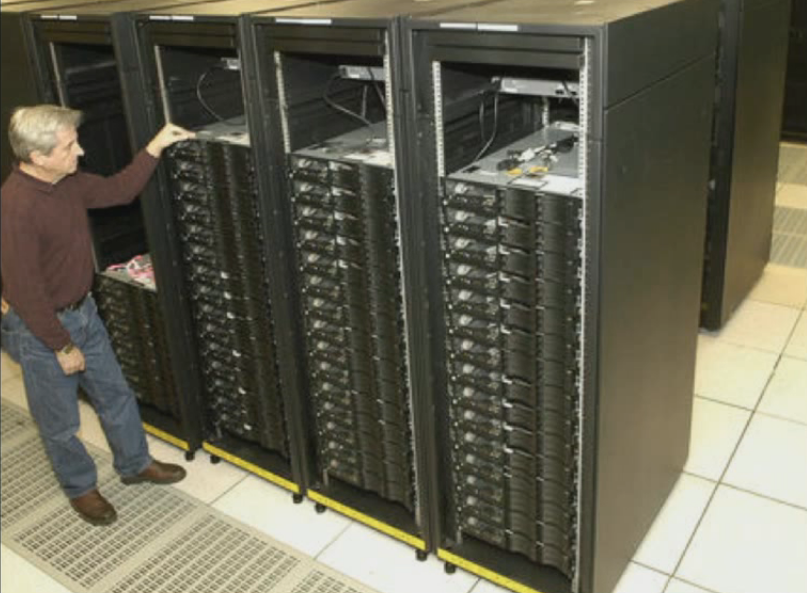
\includegraphics[width=7cm]{intro2/computer.png}
%\caption{Computing machines.} \label{introsss}
%\end{figure}

As engineers we want to build systems that are better than our brain, to point out the difficulty of this endeavor, we can summarize the brain characteristics as follows: it has 100 billion computing elements, processing and memory are performed by the same components, works as parallel recurrent paradigm, it solves problems not soluble by previous machines, and it only requires 20 watts of power.


There are several computation challenges very interesting but, despite recent success in most of them, we struggle to reach brain performance and efficiency. Machines have beaten us in extracting information for large collection of data, they can process larger amount of data than the humans. Also, in memory, they beat us, they can store more information and access faster to it than humans. It is not a matter of speed computation, they also exceed us in reasoning tasks, like playing chess or Go. However, in low-level sensorimotor skills, like seeing or walking, our brains perform better than machines. These kinds of tasks, that humans perform unconsciously, for a computer are really complex to achieve.

This fact is called the Moravec's paradox, this paradox came out during the dawn of Artificial Intelligence back in the 80s when M.Minsky, R.Brooks, and H. Moravec tried to mimic human skills by reverse engineering on the brain. This paradox says that, contrary to traditional assumptions, high-level reasoning requires very little computation, but tasks involving  perception, attention, visualization, motor, and social skills require enormous computational resources and are difficult to transfer to machines.

One possible explanation of this paradox, is based on evolution. Human skills are implemented biologically, improved over years of natural selection. The older a skill is, the more time natural selection has had to improve its design. In contrast, abstract thought was developed only very recently and it is easy to implement due this shorter development.

These categories of intelligence will take much more time to implement in machines, but research keeps going.

This master thesis lies in the context of AI and computer vision, and more precisely in the problem of visual object tracking.

\section{Computer vision}


In the late 60s, computer vision began at universities that were pioneering artificial intelligence. It was meant to mimic the human visual system, as a stepping stone to endowing robots with intelligent behaviour. In 1966, it was believed that this could be achieved through a summer project, by attaching a camera to a computer and having it \textit{describe what it saw}.

This describes the excitement of that time and their underestimation of the field. Although it is a complex area of study,there have been a lot of developments along fifty years, real world applications have been developed and are part of daily use. 

One recent application of computer vision is the usage of these techniques on robotics, in particular on autonomous cars. These cars developed by technological giants are being used in some States of US. In these systems, the surrounding information is extracted by cameras. As we can observe in figure \ref{intro1} computer vision is used to detect other types of vehicles on the road.

\begin{figure}[H]
\centering         
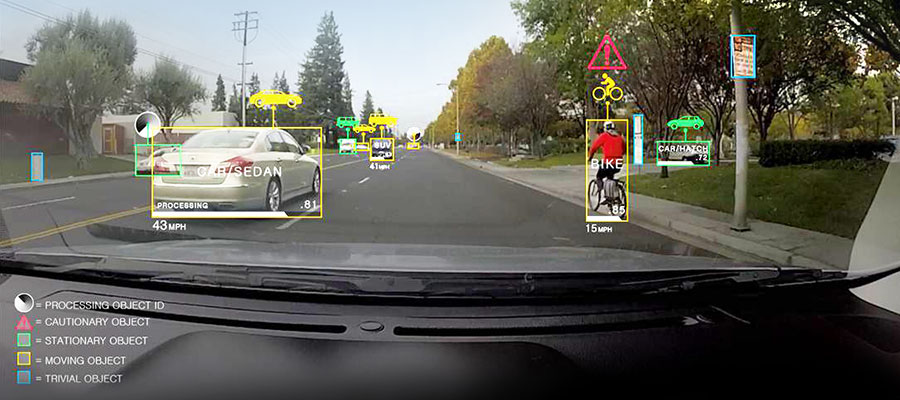
\includegraphics[width=8cm]{aplicaciones/autonomous.jpg}
\caption{Frontal view of autonomous car.} \label{intro1}
\end{figure}



Another computer vision's area is medical imaging, this area studies the techniques and process of creating visual representations of the internals of a body for clinical analysis. One example is the tractography map, like the one in figure \ref{introTractog} created from a diffusion weighted images, it allows us to establish connections between different areas of the brain.

\begin{figure}[H]
\centering         
\includegraphics[width=8cm]{aplicaciones/diffusion.jpg}
\caption{Tractography map.} \label{introTractog}
\end{figure}


One pioneer in the computer vision technology was the automation industry, where this technology is used to manufacture quicker and better. Computer vision is deeply used in factories, for instance in quality inspection of manufactured products, it can check whether a product fulfills quality characteristics, as we can observe in figure \ref{introFactory}.

\begin{figure}[H]
\centering         
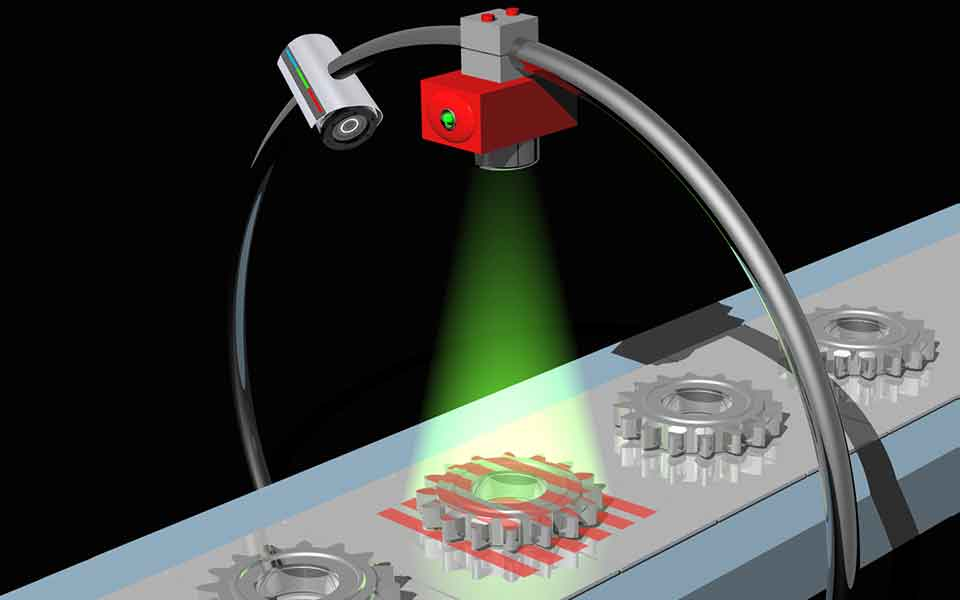
\includegraphics[width=8cm]{aplicaciones/factory.jpg}
\caption{Camera for inspection.} \label{introFactory}
\end{figure}

%
%Another application of computer vision is to get , in these types of application cameras can work by itself, but it has better results when it is combined with depth sensors. This is called RGBD sensor, it allows to estimate the depth of the scene and superimpose the texture, as we can observe in figure \ref{introrgbd}

Finally, another application of computer vision is to mix the information provided by the camera with graphics, this is called, augmented reality. One example of it is the work of the Snapchat company, it allows you to render different artifacts on an image and share it with your friends. We can observe one example on figure \ref{introrgbd}.

\begin{figure}[H]
\centering         
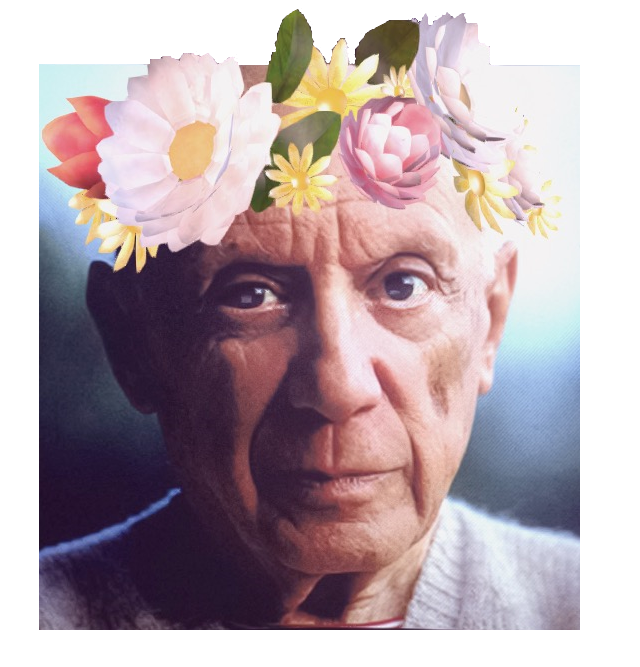
\includegraphics[width=8cm]{aplicaciones/picassioHuai.png}
\caption{Augmented reality image.} \label{introrgbd}
\end{figure}





\section{Object tracking}

In the widely computer vision field there are several study areas, one of them is Object Tracking. It estimates target state over time from image sequences. As state we can embed the position, velocity, shape, appearance or any other interesting characteristic. It is very challenging field due to:


\begin{itemize}

\item Variations because of geometric changes, some targets might be deformed as they move in the scene which would change their structure.

\item Variations due to photometric factors, the appearance of the targets might change due to changes in illumination.

\item Occlusions, targets might mix with other elements of the scene from the camera perspective.

\item Image quality, the image sequences could incorporate noise or low resolution.

\item Similar objects in the scene, this could cause problems to maintain the identity of targets.

\end{itemize}

To solve these problems the community has used the several paradigms:

\begin{itemize}

\item \textbf{Tracking using matching}, this kind of methods performs a matching of the representation between the current and the possible candidates in the next frame. Key points of these methods are the representation and the similarity measurement helps to perform the matching. Maybe the most famous methods are Normalized Cross-Correlation \cite{trackNcc}, Lucas-Kanade tracker \cite{klt}, Kalman appearance tracker \cite{kalmm} and Mean shift tracking  \cite{meanshift}. 

\item \textbf{Tracking-by-detection}, this kind of methods builds a classifier to distinguish target pixels from the background. Once you have the detection, you need a data association method to link those detections. Traditionally the community has used kernel methods with support vector machines \cite{struc} to perform the detections, but in the recent years people are shifting to neural networks. In the data association algorithms graph theory techniques are dominant \cite{dataAsso1} \cite{dataAsso2}.


\item \textbf{Tracking learning and detection}, this is an extension of the previous category. It includes a mechanism to update the classifier during the execution of the system. This learning procedure allows the algorithm to be invariant to changes in the target. Maybe the most famous algorithms are the Predator \cite{tld} and the Alien \cite{alien}.



\end{itemize}


These kinds of algorithms are quite mature and are deployed in real life applications. Like several the computing applications they allow us to process a huge quantity of information really quickly.

In video surveillance, Object Tracking allow us to track all the targets without human intervention and notify when there are dangerous situations. 

\begin{figure}[H]
\centering         
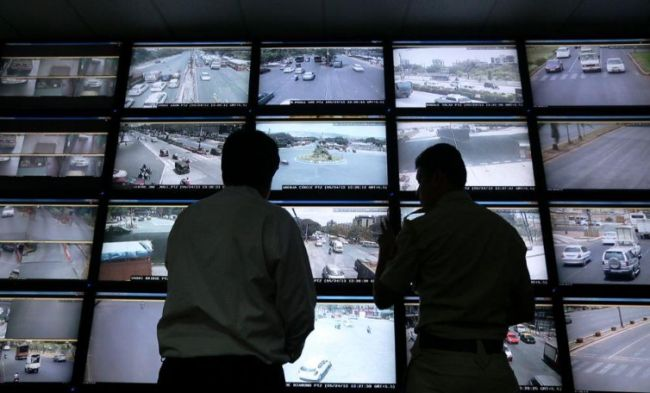
\includegraphics[width=8cm]{aplicaciones/policias.jpg}
\caption{Control room.} \label{introTracking1}
\end{figure}


For science, they allow us to study the environment, in the case of the figure \ref{introTracking2}, for humans it will be difficult avoid missing the correct identity of any ant. With information supplied by the tracking, scientist can study how animals move and interact with others.

\begin{figure}[H]
\centering         
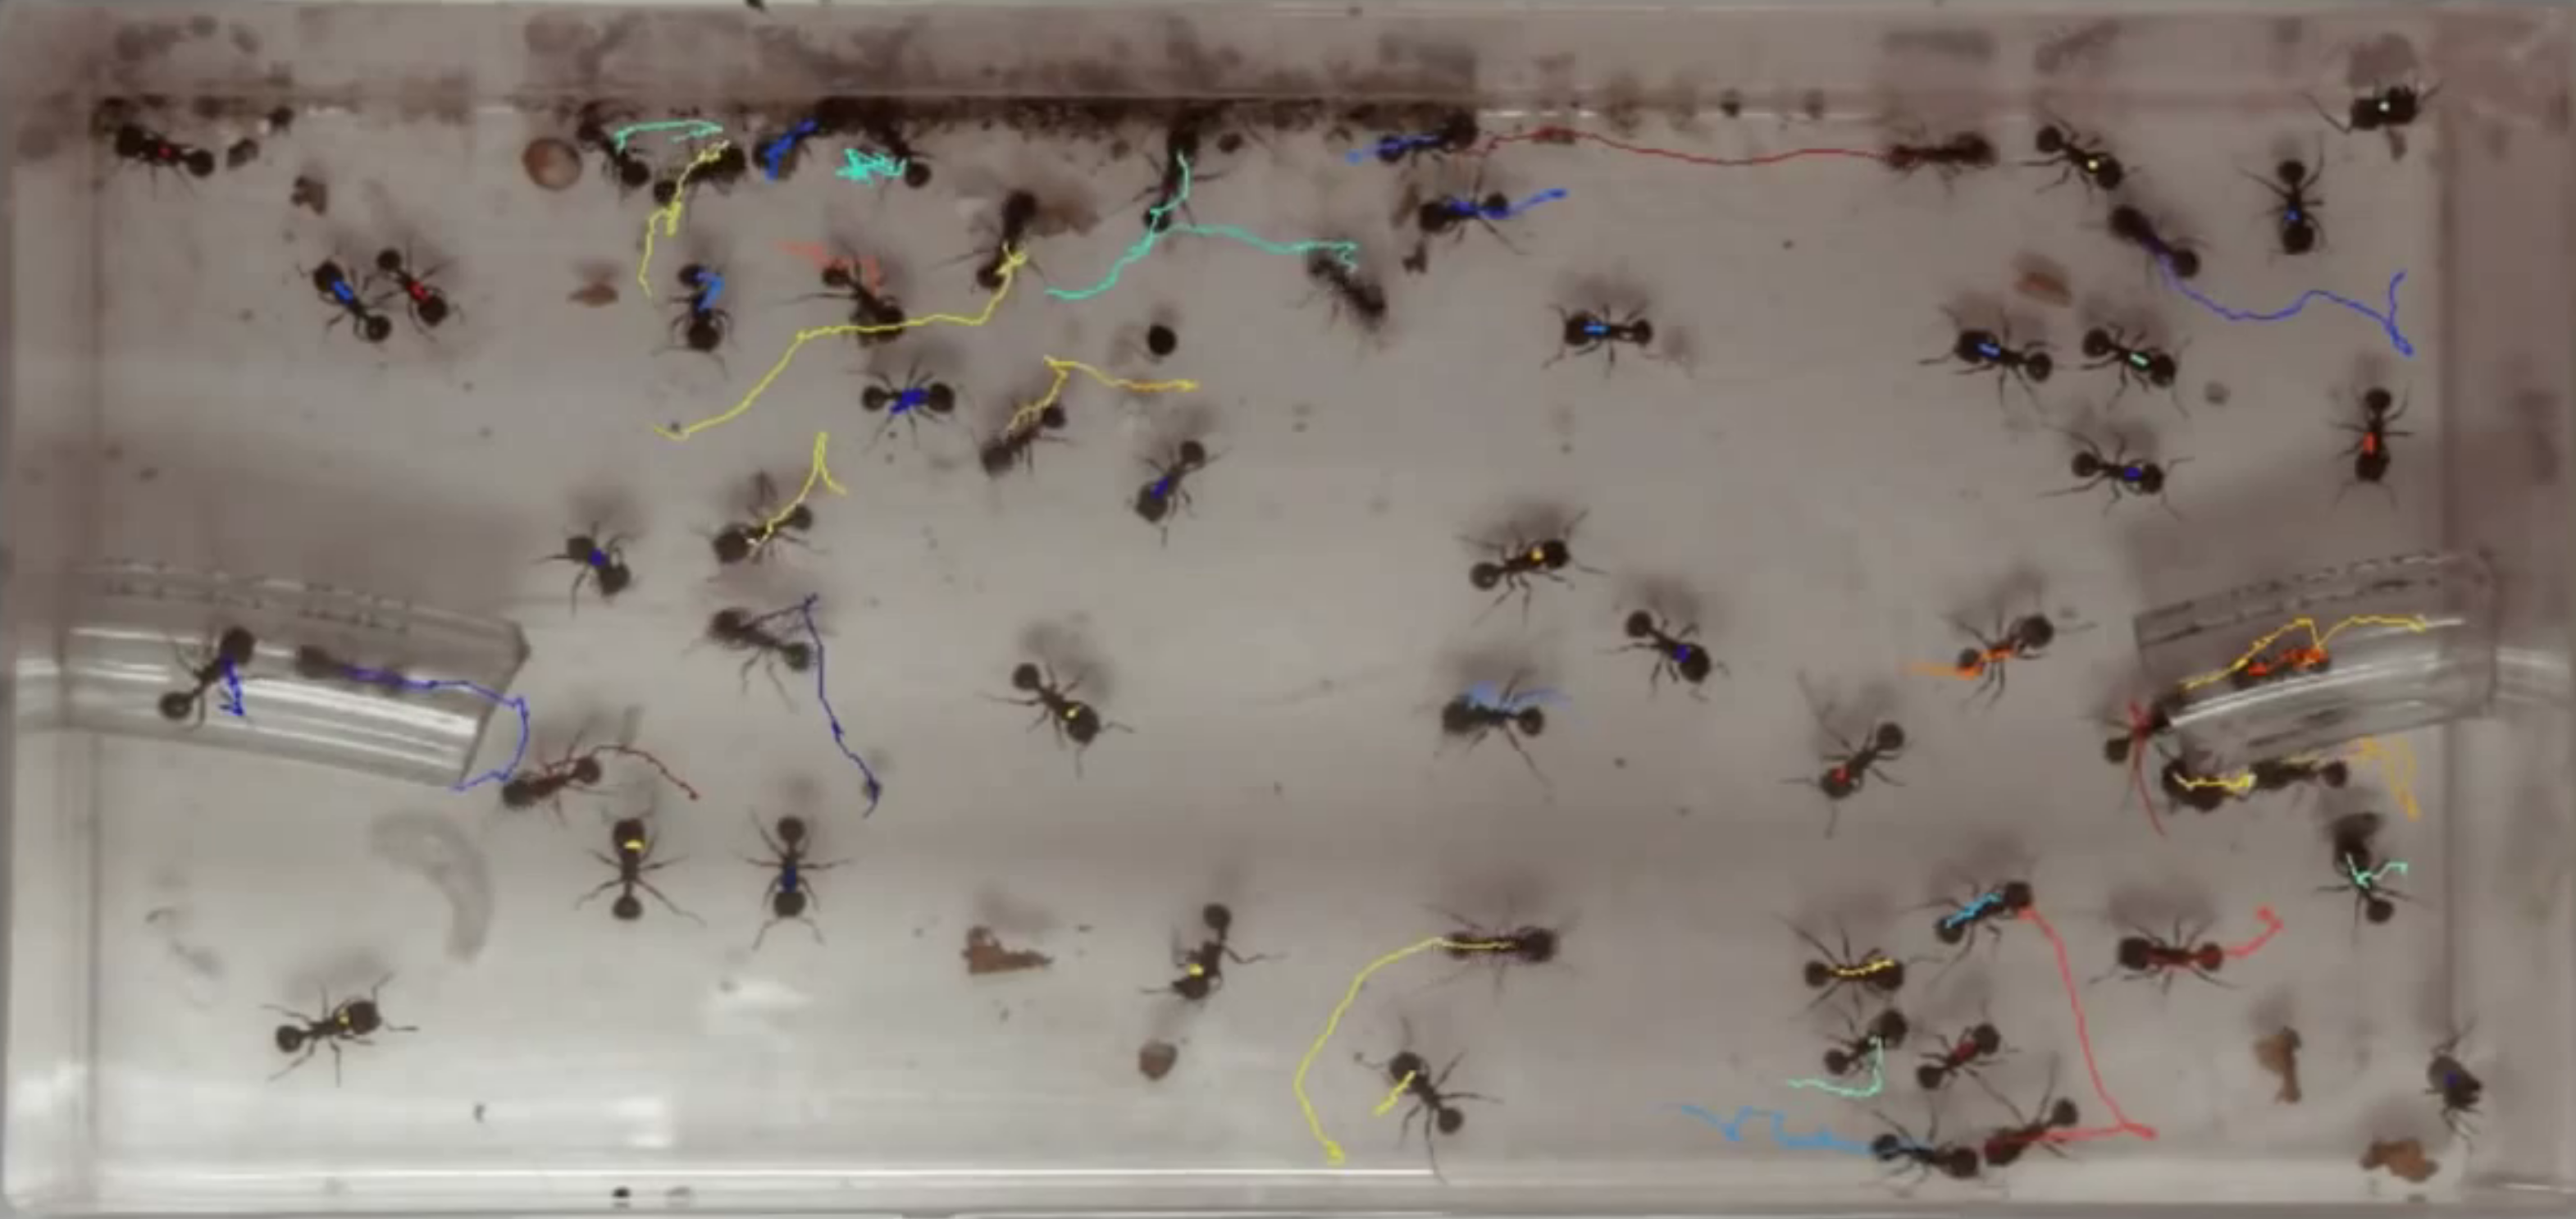
\includegraphics[width=8cm]{aplicaciones/Seleccio_007.png}
\caption{Visual tracking for science.} \label{introTracking2}
\end{figure}

These algorithms are deeply used in all kind of sports like the NBA and NFL. In these situations the algorithms track the players during the game and allow to analysis his/her performance and the strategy of the team, like in figure \ref{introTracking3} .

\begin{figure}[H]
	
\centering

\subfigure[Input image]{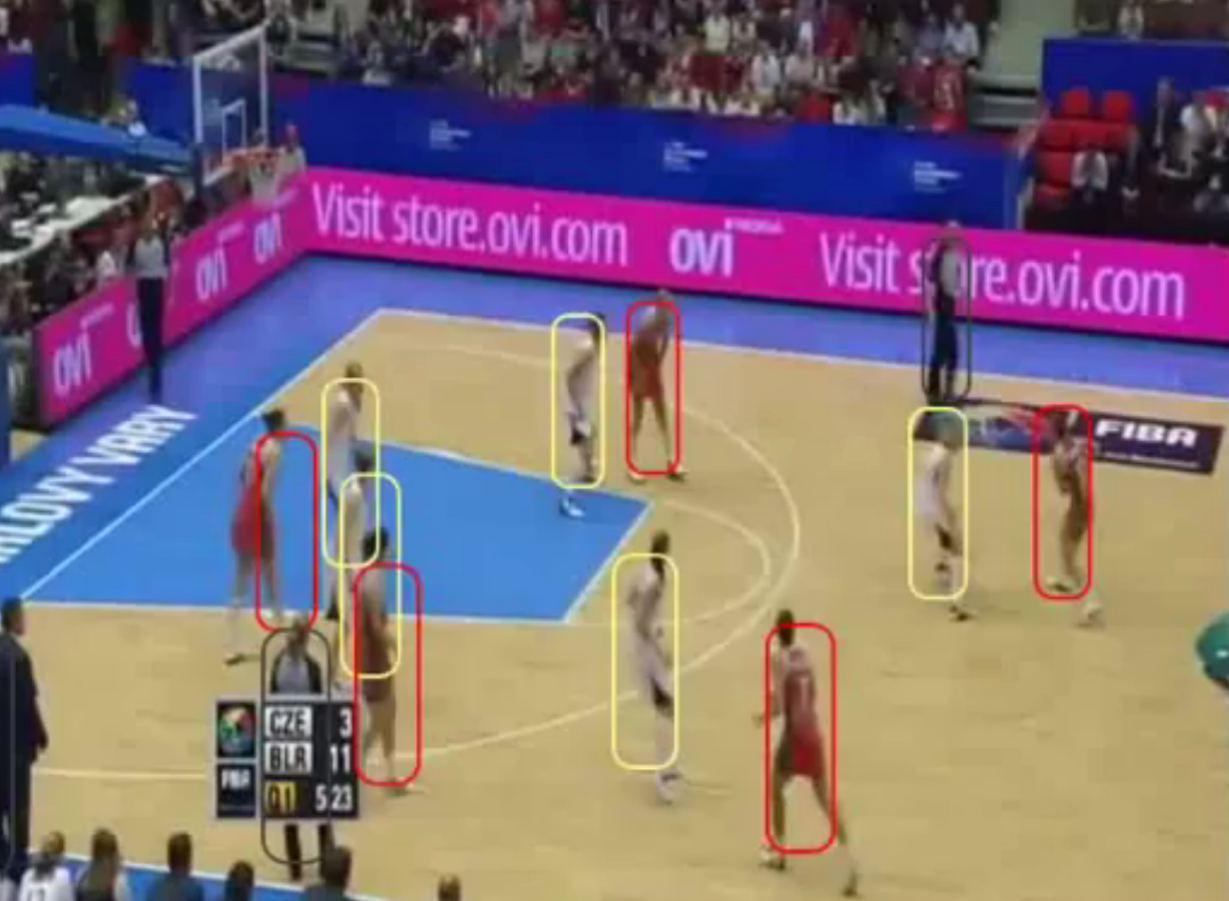
\includegraphics[width=5cm]{aplicaciones/Seleccio_010.png}}
\subfigure[Layout ]{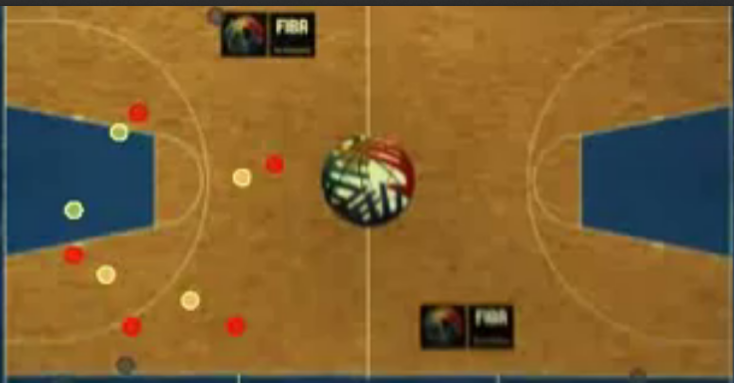
\includegraphics[width=7cm]{aplicaciones/Seleccio_011.png}}\\


\caption{Visual tracking for sports analysis.}
\label{introTracking3}
\end{figure}

In artistic performance, these algorithms are used to track the subject and render some graphics in the scene, like an extension to video of augmented reality. In the example of the figure \ref{introTracking4}, the systems track the singer's head and projects a visualization of his voice.

\begin{figure}[H]
\centering         
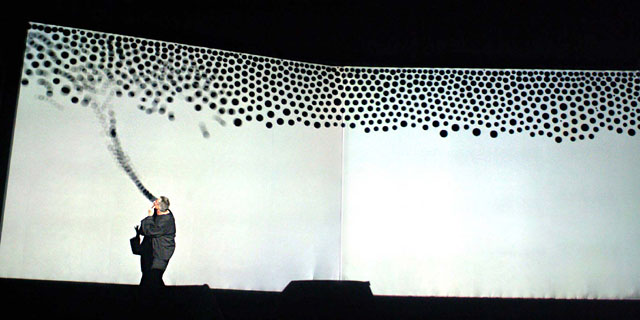
\includegraphics[width=12cm]{aplicaciones/singing.jpg}
\caption{Visual tracking for art.} \label{introTracking4}
\end{figure}


\section{Deep learning in computer vision}

Deep learning has raised by drastic improvements over reigning approaches towards the hardest problems in Artificial intelligence (AI). It has gathered massive investments from industry giants, and exponential growth in research publications. Deep learning is a tool inside the machine learning toolbox, whose goal is to make machines learn.

The first incursion was made by Frank Rosenblatt, the Percetron \cite{rosenblat}. Rosenblatt conceived the Percetron as a simplified mathematical model of how the neurons in our brains operate. This model of the neuron built on the work of McCuloch-Pitts \cite{McCulloch}, who showed that a neuron model could replicate the basics OR/AND/NOT functions. That was great in the early days of Artificial intelligence, because the predominant thought at that time was that making computers able to perform formal logical reasoning would essentially solve AI. However, the McCuloch-Pitts model lacked a mechanism for learning, which was crucial for it to be usable for AI. This is were the Perceptron suceeded, Rosenblatt came up with a way to make such artificial neurons learn, inspired by the Hebb's Rule. This learning method was as follows: if the output of the perceptron was low, increase the weights, otherwise decrease the weights if the output is too high. Also, another researchers came with ADALINE \cite{adaline} learning procedure. They used the signal before the activation function to compute the derivative, how much the error changes when each weight is changed can be used to drive the error down and find the optimal weight values. This is similar to the way we train the networks nowadays.

Researchers were really excited about this idea of Connectionism: those networks of such simple computational units could be vastly powerful and solve the hard problems of AI. But in 1969, Minsky and Papert  published an analysis on the limitations of perceptrons \cite{minsky69perceptrons}. The biggest criticism was that a perceptron could not learn the simple boolean function XOR because it is not linearly separable. However, they stated that it could be learnt with multiple layers perceptron but the learning procedure did not work for multiple layers. After this book, the interest on Neural networks decreased, and it initializes a period called \textit{AI winter}, AI shifted to logic programming and common sense reasoning.

This period lasted till 1986 when Rummelhart, Hinton, and Williams published the algorithm of backpropagation \cite{Rumelhart}, which specifically addressed the problems discussed by Minsky in Perceptrons, a method to train multiple layer neural nets. With this discovery in 1989, LeCun showed a real world application, recognized handwritten digits \cite{lecunZip}. The architecture of this model was a convolutional neural network. It was inspired by the Neurocognitron \cite{Fukushima} of Fukushima, which took ideas from studies of the brain. In particular, the studies of Hubel and Wiesel, they propose that the visual cortex is formed by a hierarchical model, primarily for simple cells that respond for simple structures and then complex cells that respond to a more complicated feature. As we can observe in figure \ref{intro1}, in the lower layer, the network learns Gabor like features, and while going upwards, the networks learn more abstract concepts.




\begin{figure}[H]
\centering         
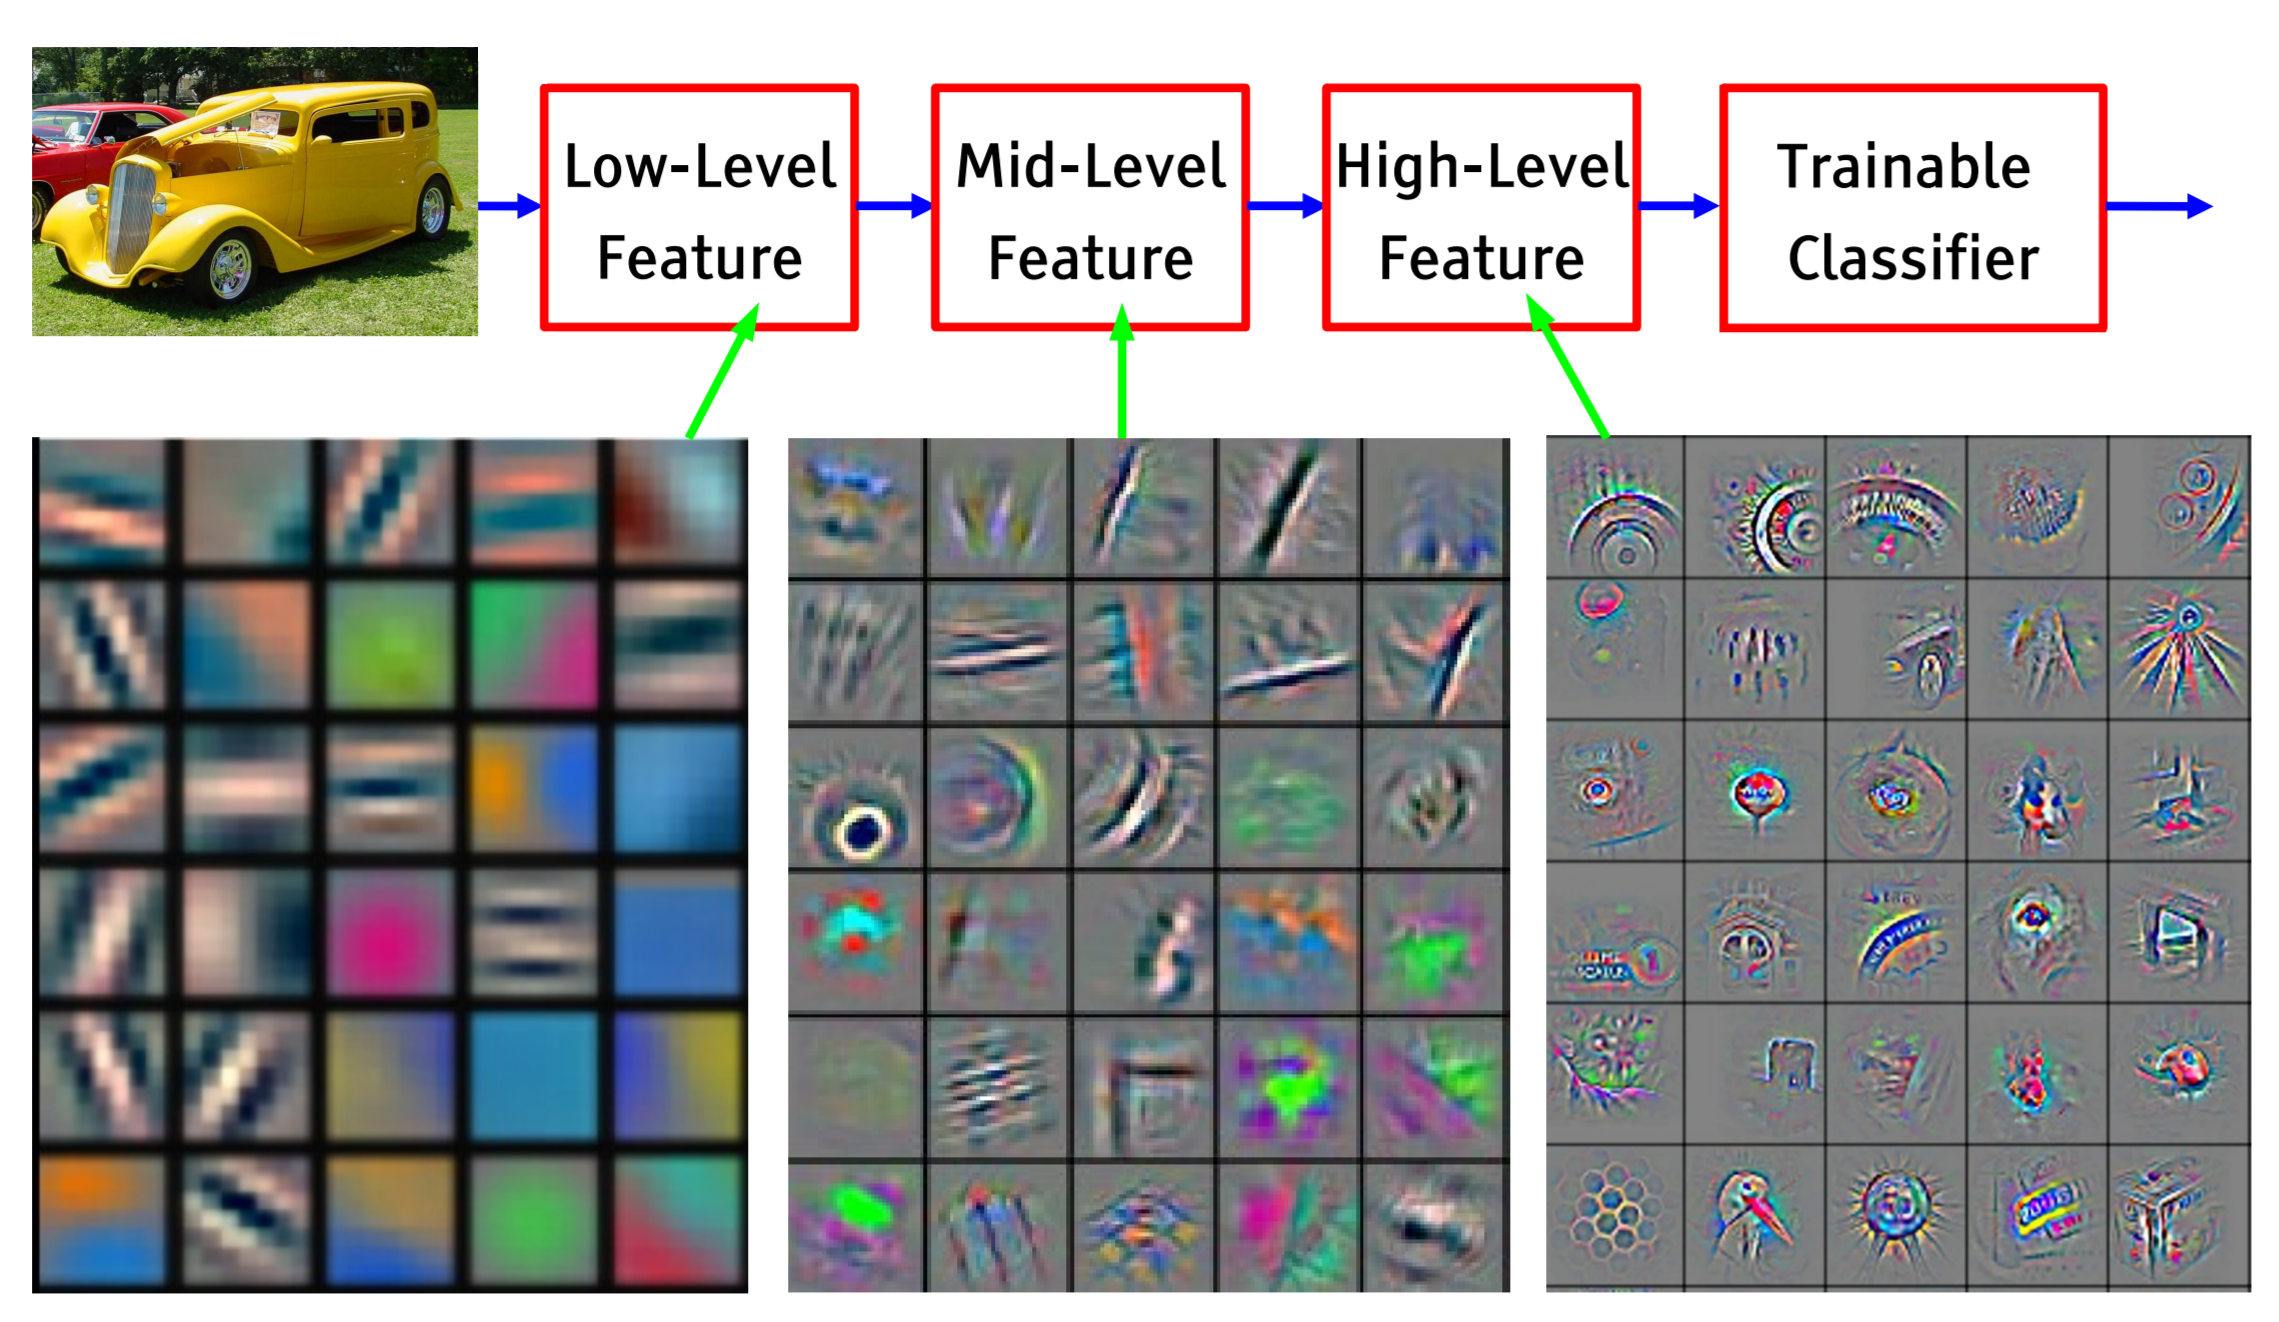
\includegraphics[width=12cm]{intro/model.png}
\caption{Representation of a Convolutional neural network.} \label{intro1}
\end{figure}



But this approach did not scale to larger problems, the biggest source of problems was the vanishing gradients problem. When the backpropagation gradients backpropagates trough the network, in some nodes the local gradient is very low ( in the extreme of the sigmoid functions ) and the signal vanishes or saturates. By the 90s other techniques became the method of choice, like support vector machine (SVM), although some progress was made for other kinds of problems.

\begin{itemize}

\item Unsupervised learning. This type of architectures is used to find a smaller representation of some data from which the original data can be reconstructed, it is useful for compression, visualization, and classification. One example of this architecture with neural networks is the Restricted Boltzmann machine \cite{boltzmann}, developed by Hinton.
%in this setting the neurons behave according to a probability distribution, and form a graphical model. The neuron are hidden %layers, and it can be used to infer information from it.
 
\item Reinforcement learning. The goal of this type of learning is to learn how to make good decisions, it requires rewards, not labels. One example of this sort of systems, is the TD-Gammon \cite{Gammon}, a neural network that learned to be a backgammon player.

%\item Robotics. This was another field separate from Machine Learning where neural nets were very useful. A major example of early neural net use for robotics came from CMU's NavLab in 1989. the neural net learned to control the vehicle using steering data recorded while a human drove \cite{alvin}.

\item Recurrent neural networks. Plain neural networks could not process sequences due to they do not have memory, they need mechanism to remember the pasts outputs. With memory, it can process sequences like audio or text. One approach to this is Waibel \cite{Waibel} in 1989. 


\end{itemize}


In 2006, there was a breakthrough \cite{hinton06}, Hinton realized that a neural network with many layers really could be trained well if the weights are initialized in a clever way. The basic idea was to train each layer one by one with unsupervised training ( like an autoencoder architecture ) and finally stack all together and train it in a supervised way. 

Although these improvements, the big step forward came in 2012, when AlexNet \cite{alexnet} beat the state of the art in the ImageNet challenge, an image classification challenge, where the error rate was $15.3 \%$ whereas the winner of the previous year was $26.3 \%$. In the figure \ref{intro2} we can observe the advance in the state of the art of the ImageNet challenge with the inclusion of deep learning techniques.




\begin{figure}[H]
\centering         
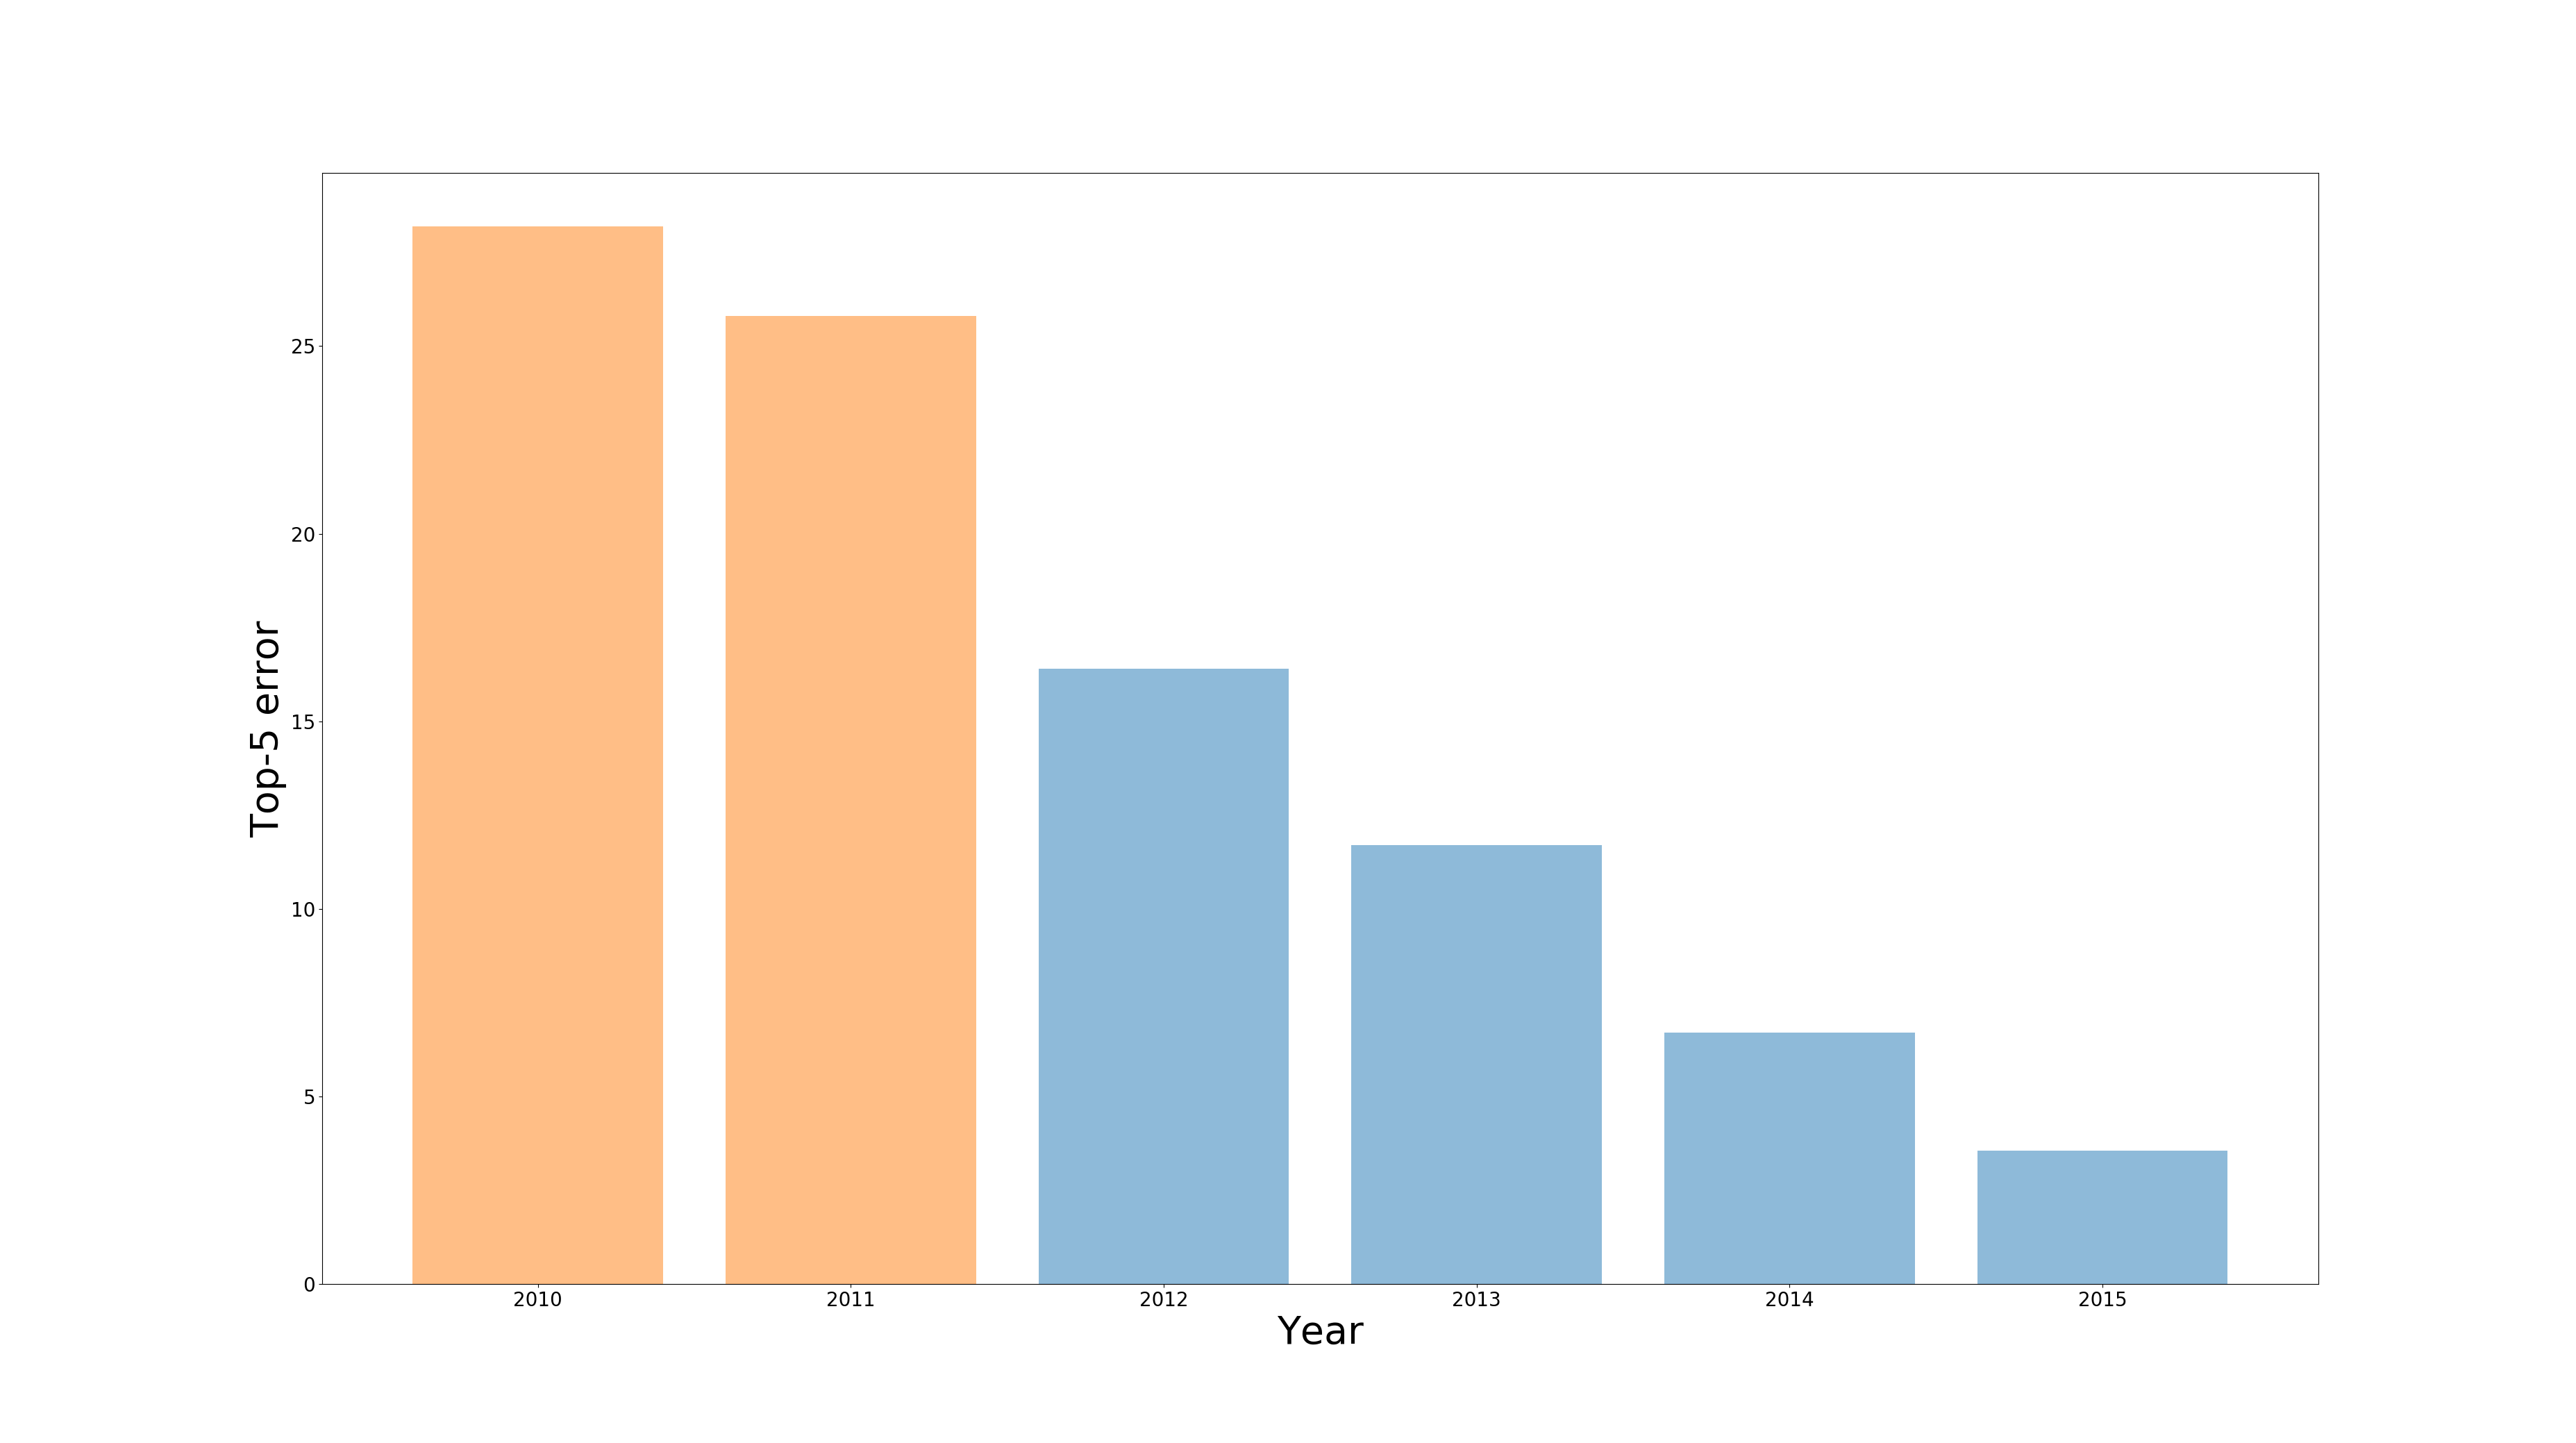
\includegraphics[width=0.7\linewidth]{intro/iamgeWihtou.png}
\caption{Classification error in ImageNet challenge.} \label{intro2}
\end{figure}



The emergence of these techniques were the culmination of decades of research but the step forward was due by three aspects:

\begin{itemize}

\item \textbf{Appearance of large and high quality datasets}, The increasing size and quality of the datasets help the networks to converge easily.

\item \textbf{Parallel computation}, The increasing of computing capabilities helped train larger models in less time.

\item \textbf{Optimization details}. With the discovery of the proper initialization and activation functions larger networks can be trained.


\end{itemize}














\lhead[]{CAPÍTULO \thechapter. Objetivos}
\chapter{Objectives}\label{cap.objetctives}

Once we put in context our work, in this chapter we explain the objectives of this thesis, its requirements and the methodology to accomplish it.


\section{Objective}

The main objective of this thesis is to develop and characterize an algorithm of multiple people tracking with two diferents methods: deep learning techniques and feature tracking. The essence of this work is study how combine it, and reach real time operation and a high performance. Finally, validate our solution with a international dataset, the Multiple Object Tracking dataset. We divided this target in several sub-objectives:

\begin{itemize}


\item \textbf{Object detector using deep learning}. Study the fundamentals of object detectors with deep learning techniques. We analyzed the performance on the main datasets and finally, we chose one to our task. 

\item \textbf{Development of a tracking module}. We studied which tracking technique would fit our problem, when it was selected, we implemented on code.

\item \textbf{Join these two techniques}. We integrated this two techniques to perform a complete tracking algorithm.

\item \textbf{Test the component on an international databases}. We validate our solution on well-known database. 


\end{itemize}

\subsection{Requirements}

In addition to the previous objectives, our solution must satisfy the following requirements:

\begin{itemize}

\item The solution will make use of the JdeRobot framework, release 5.5, which is the developing environment of the \textit{Grupo de Robótica} of the \textit{Universidad Rey Juan Carlos}.

\item The software will run on the GNU/Linux Ubuntu 16.04 environment.

\item The algorithm will only make use of video sequences not other information.

\item The algorithm must achieve an execution on real time and guarantee a precision.


\end{itemize}

%\section{Working plan}
%
%In this part we explain chronologicaly our work to develope our thesis.
%\begin{itemize}
%
%
%\item \textbf{Object detector using deep learning}. Study the fundamentals of object detectors with deep learning techniques. We analysed the performance on the main datasets and finally, we chose one to our task. 
%
%\item \textbf{Development of a tracking module}. We studied which tracking technique would fit our problem, when it was selected, we implemented on code.
%
%\item \textbf{Join these two techniques}. We integrated this two techniques to perform a complete tracking algorithm.
%
%\item \textbf{Test the component on an international databases}. We validate our solution on well-known database. 
%
%
%\end{itemize}



\section{Methodology}

To achieve our objectives we used several tools that helped to monitoring the project for all members of the team. It allowed to comment or correct the task.

The main tool, it has been the videoconference, we established a weekly meeting with all the members of the team. In this meetings we showed the results and we shared our feedback with the other members of the team. 

As complementary tools, we used a website and Github repository, these tools helped to control the development of our work. The website was developed using the wiki of JdeRobot \cite{wikiPieras}, this shows the weekly tasks and results. The Git Hub repository \cite{repoPieras} allows to access to the code by all the members of the team.

Our development plan was based on the Spiral model. It consists in four steps. In the first step, we determine the objectives of our project, in the second one, we analyze the risks and evaluate which problems we will face, then we develope and test our prototype and the last step consists to evaluate the results. We apply several iteration of this process till we get a satisfactory project.


































\lhead[]{CAPÍTULO \thechapter. Teorethic}
\chapter{Theoretical background}\label{cap.theoretic}

In this chapter we explain the theoretical concepts of our work, these include the theory of tracking and person re-identification.

\section{Tracking}


As we explained in previous chapters, there are a traditional family of methods to solve the tracking problem. But with the incursion of deep learning techniques, they have been adapted to it and create new paradigms. The main ways to apply deep learning techniques to tracking are the following \cite{thrun}:


\begin{itemize}


\item \textbf{Tracking-by-detection}. These methods use a specific class classifier and there is not need to train it online. So, these methods use a neural network to extract instances of the frames and then linked with temporal restrictions. 

\item \textbf{Tracking learning and detection}. Starting from the first frame of a video, a tracker will sample patches near the target object, and they are used to train a foreground-background  classifier, and this classifier is used to score patches from the next frame to estimate the new location of the target object. These methods showed a state-of-the-art performance results. Unfortunately, neural networks are slow to train, therefore the speed of the method is reduced \cite{deep1} \cite{deep2}.


\item \textbf{Siamese based tracking}. In this approach, many candidate patches are passed through the network, and the patch with the highest matching score is selected as the tracking output \cite{trackingSiamese}.


\item \textbf{Tracking as regression}, these methods are an extension of object localization using neural networks, these methods given an image containing an object predict the bounding box which contain the object in every frame \cite{thrun}. They are restricted to one object.


\item \textbf{Tracking with RNN}. From the output of an object detector, these tracking algorithms model the sequence of movement of objects using an recurrent neural network \cite{savaresee}. These methods represent the current state of art in tracking.


\end{itemize}



For this thesis we chose the tracking-by-detection paradigm. We get the detections with a object detector based on deep learning networks, and we link those detections with a tracking by matching, particularly, tracking by feature.

\subsection{Detection in tracking}\label{trackingBounding}


In object detection too, the emergence of the neural networks has supposed a turning point. As we can observe in \ref{deepObjet}, the mean average precision, has almost doubled since the appearance of deep neural networks.


\begin{figure}[H]
\centering         
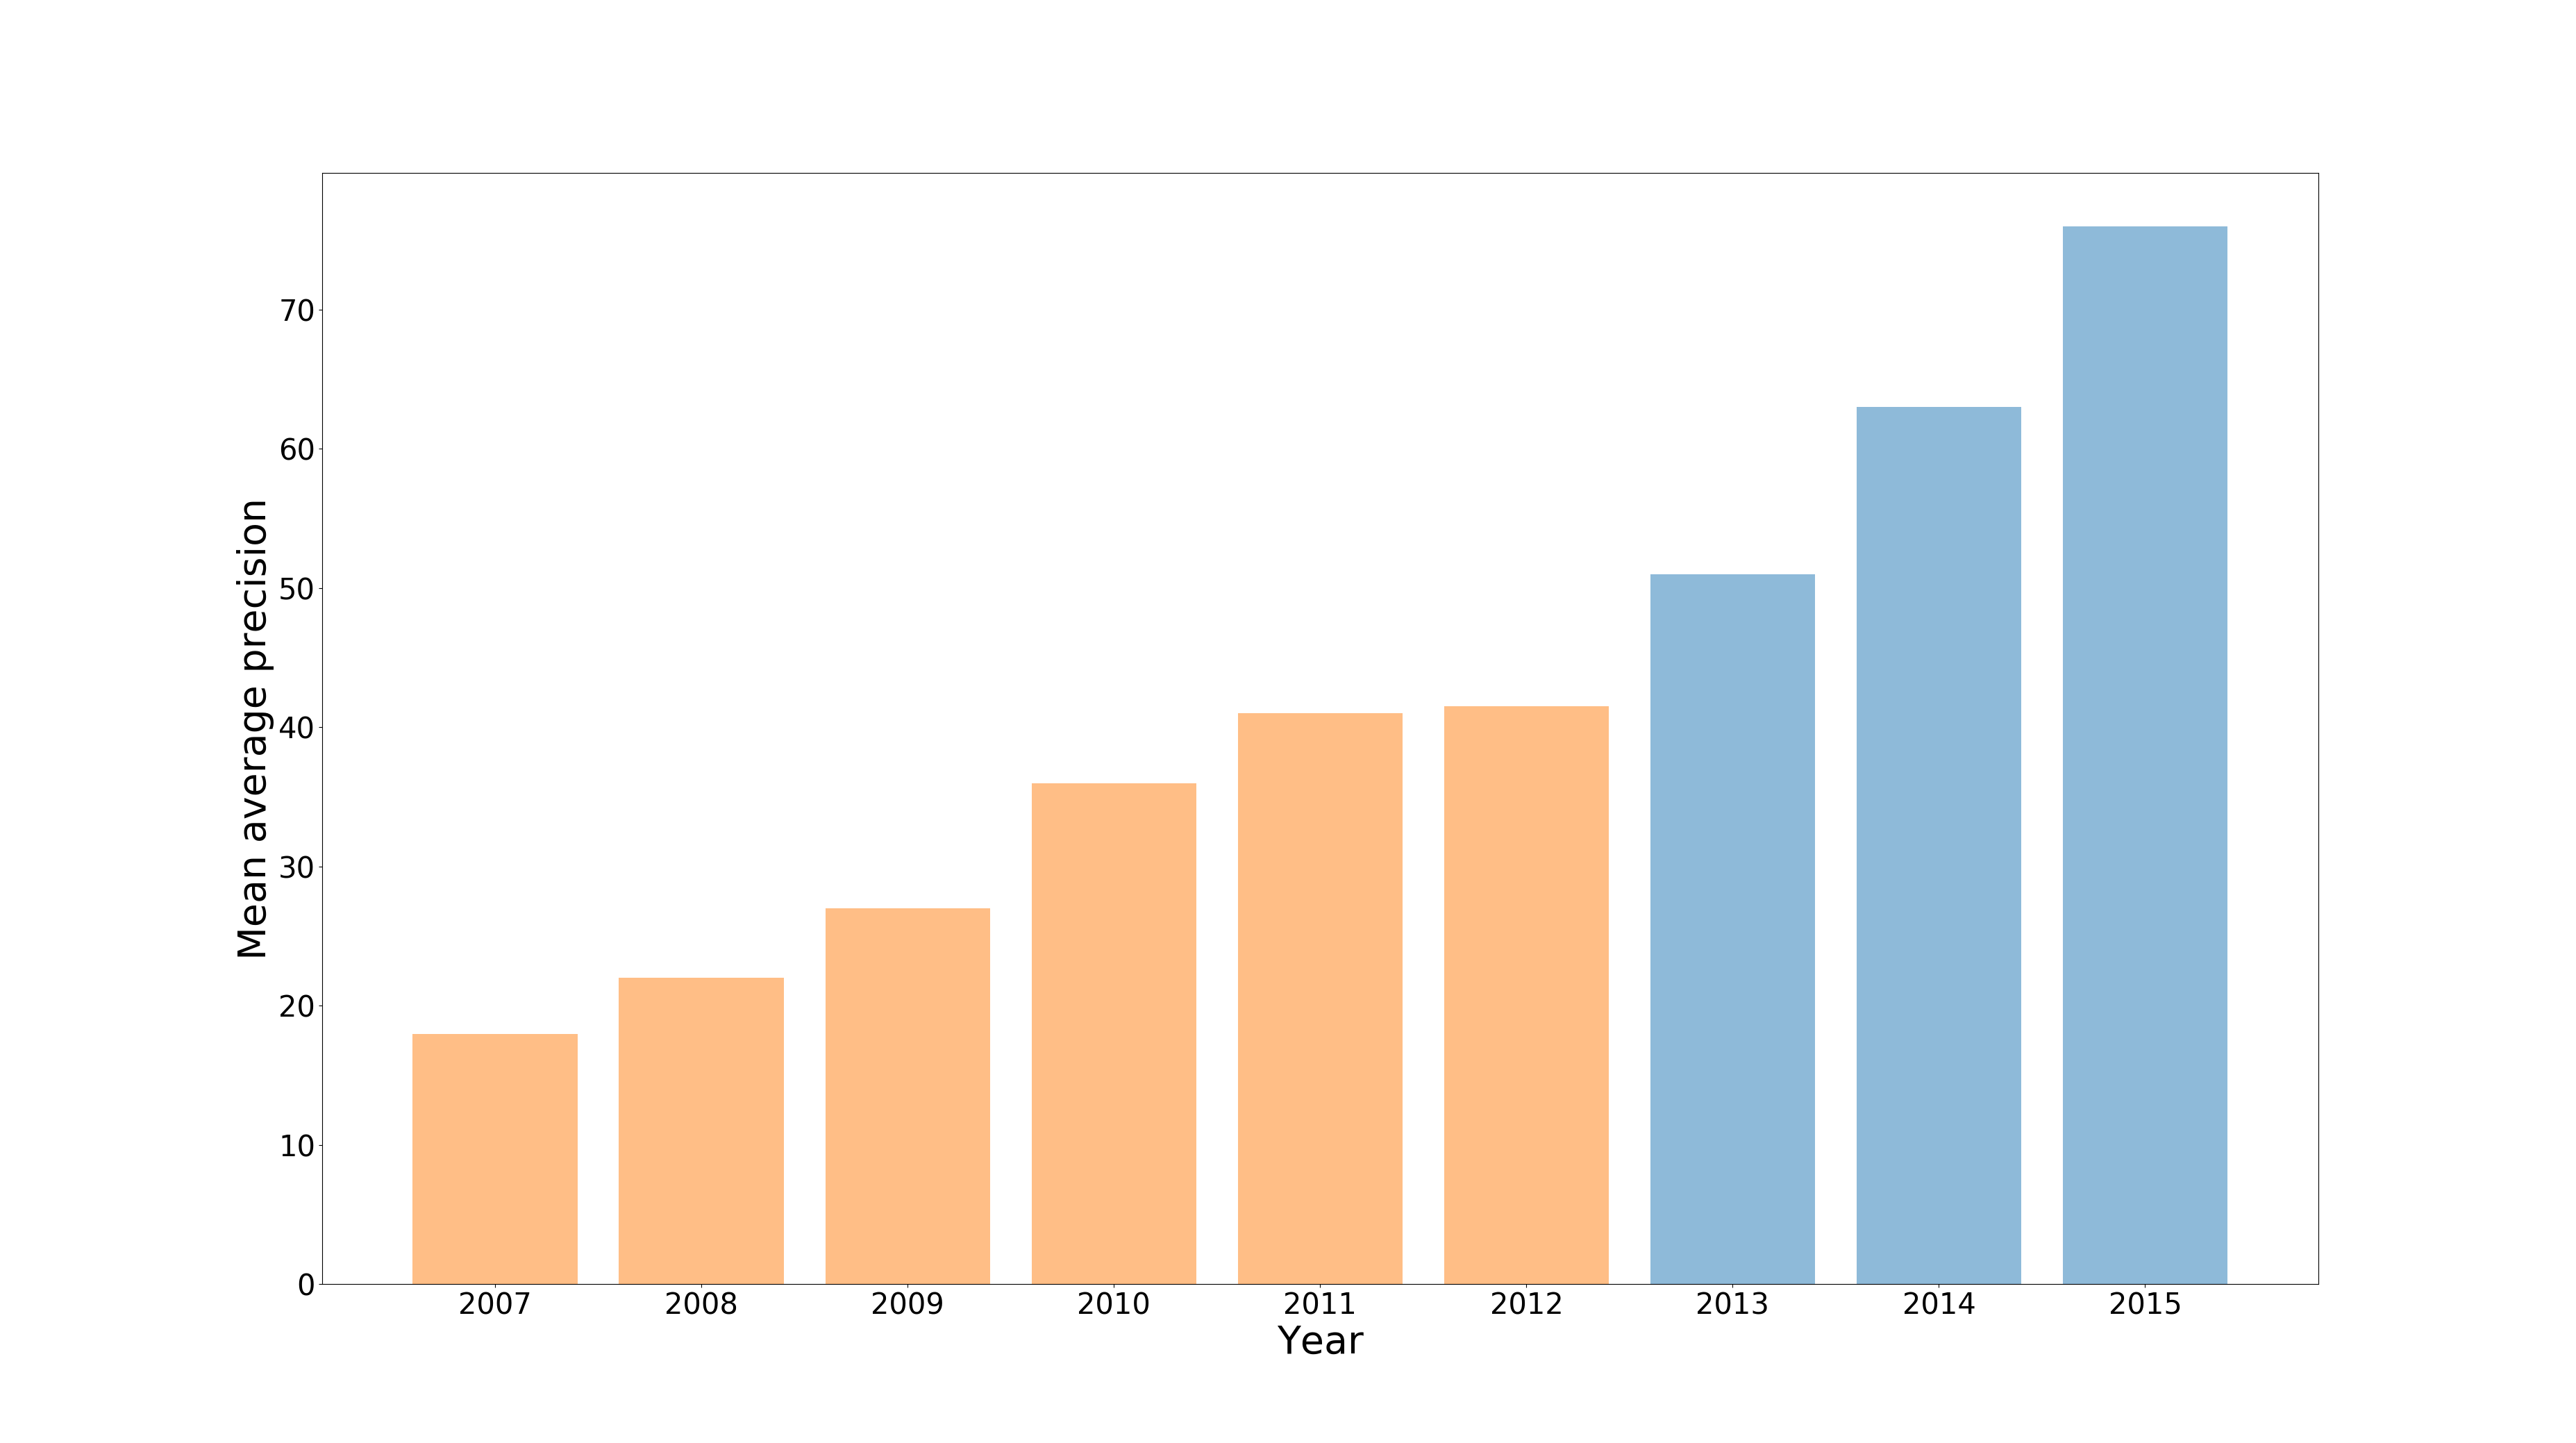
\includegraphics[width=0.7\linewidth]{intro/objesName.png}
\caption{Mean average precision over the years in PASCAL dataset.} \label{deepObjet}
\end{figure}


%Actual object detectors are based on three main family of architectures \cite{cnnComparision}, of which names are: FasterRCNN, RFCN, and SSD. In \ref{refArchite} we can observe a scheme of these systems.


Present deep learning object detectors are based on three main family of architectures \cite{cnnComparision}, named by the reference algorithm of the category: FasterRCNN, SSD, and RFCN, the characteristics of these systems are:

%\begin{figure}[H]
%		
%\centering
%
%\subfigure[Faster RCNN.]{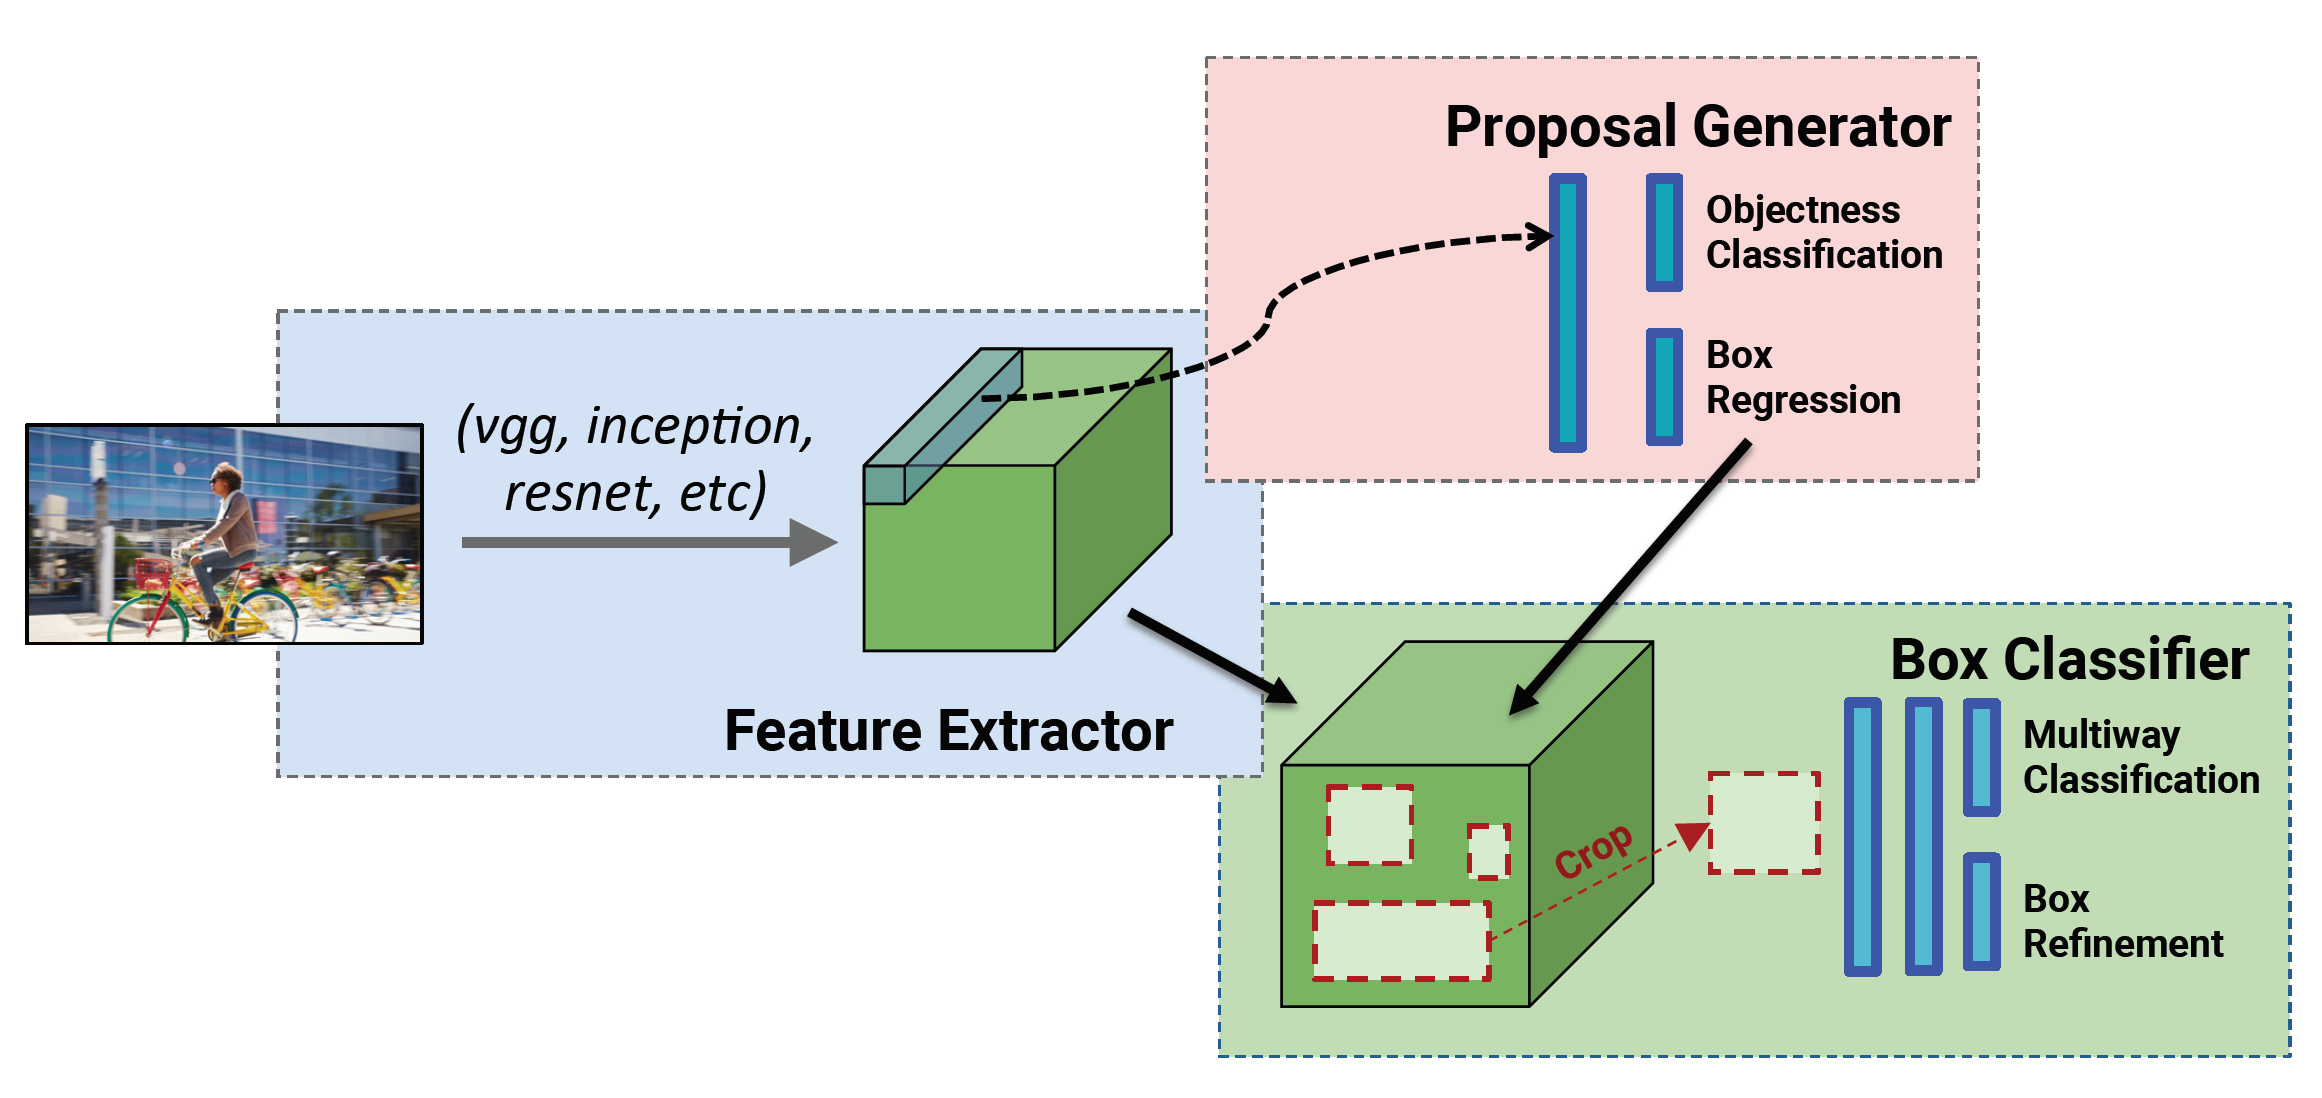
\includegraphics[width=5cm]{objectDetection/compFaster.png}}
%\subfigure[SSD.]{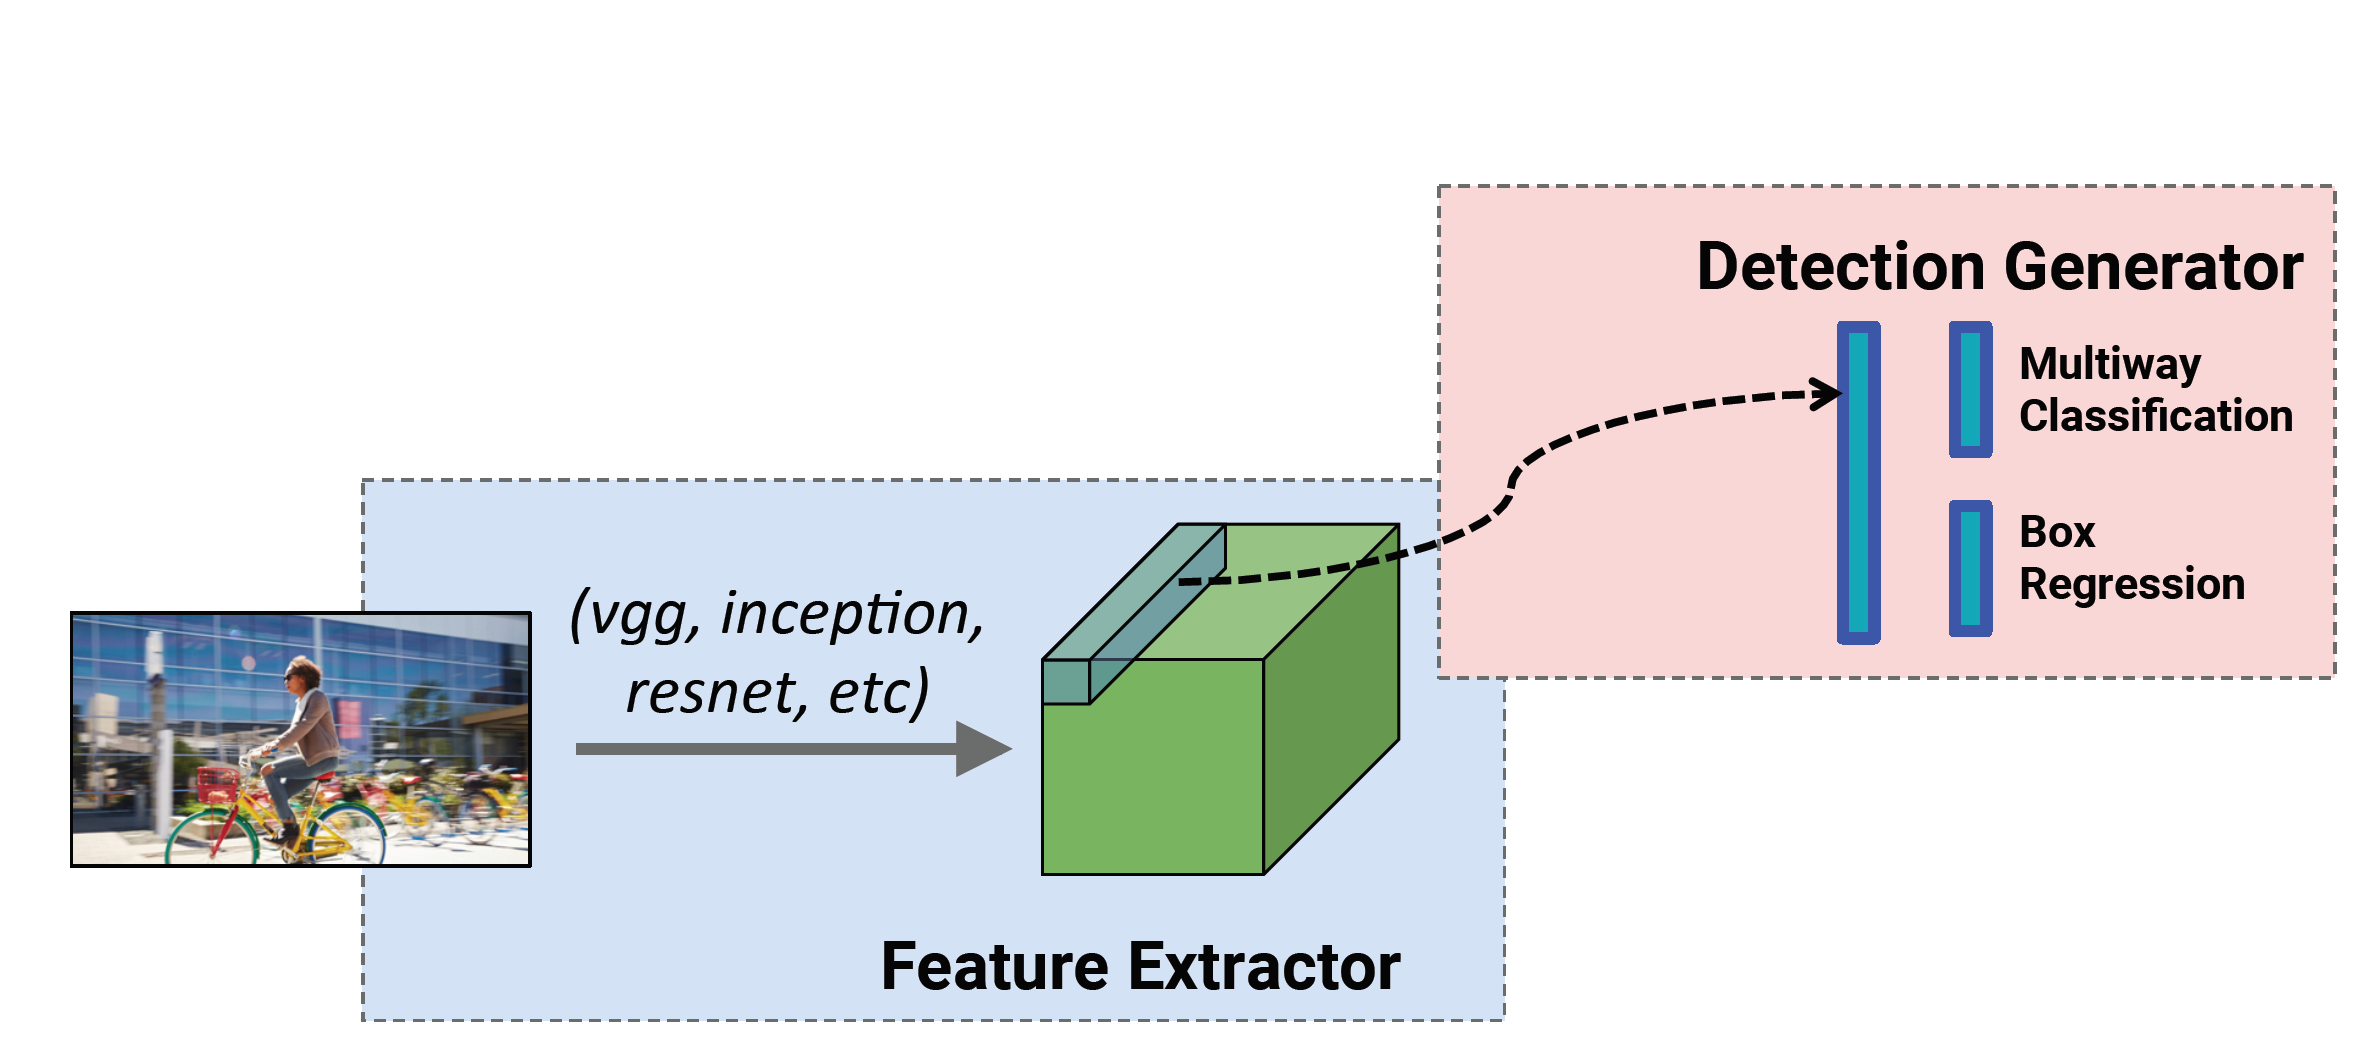
\includegraphics[width=5cm]{objectDetection/compSSD.png}}
%\subfigure[RFCN.]{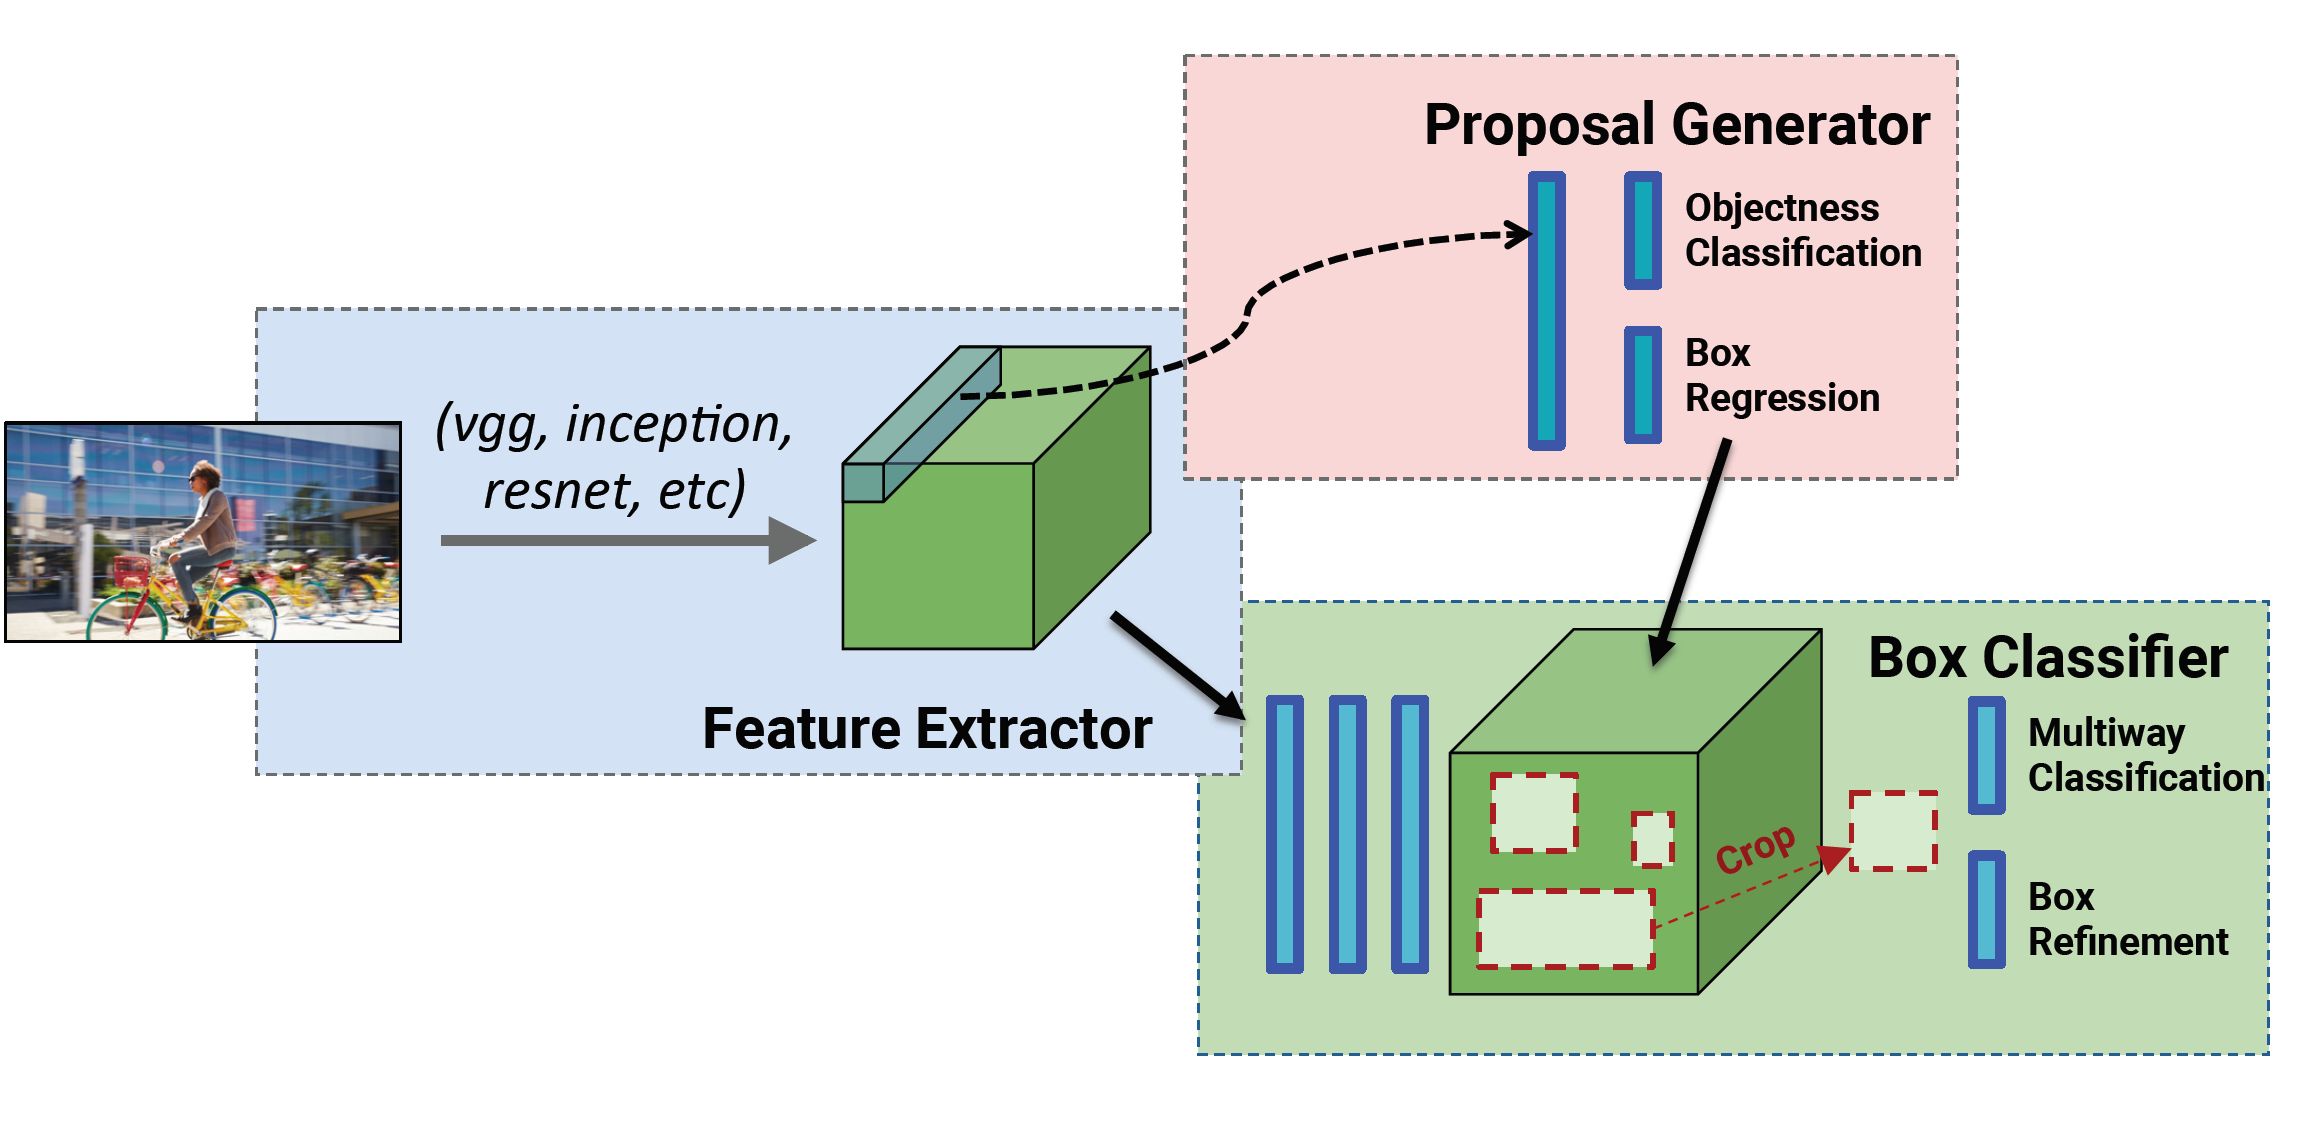
\includegraphics[width=5cm]{objectDetection/compRFCN.png}}\\
%
%\caption{Object detection architectures.}
%\label{refArchite}
%\end{figure}



\begin{itemize}

\item Faster RCNN \cite{fasterrcnn}, it is the last output of a trilogy of detectors developed by R. Girshick and his team. Which are called Region-Based object detectors. They work as follows: Use some mechanism to extract region of an image that are probable to be an object and then classify those proposals with a CNN. The first paper to do so, was \cite{rcnn}, and suppose a breakthrough in the field, increasing the precision of the state of the art of those days. But, it had a messy pipeline, slow and difficult to train. Later on, they developed \cite{fastrcnn}, in this paper they applied the region proposal algorithm in the cnn feature map, so, they avoid to compute the features for each proposal. They increase the speed and it could be trained much easily. Finally, they showed FasterRCNN \cite{fasterrcnn}, in this algorithm, they eluded the external region proposal algorithm and they implemented a CNN to compute those proposals. This CNN share parameters with the main net and they saved a lot of time. This network, has become the standard object detector with CNN. With the association of novel net architecture like ResNet \cite{resnet}, Inception \cite{inception}, and \cite{pvanet} they have won all the contests.


\item SSD, it stands for Single shot multibox detector. These family of method differs from previous ones considering that these treats the problem of object detection as a regression problem. So, they are called Regression-based object detector or single shot object detector due it does not have a region proposal algorithm, they classify the image with one mechanism. The maximum exponent of these algorithms are \cite{yolo} and \cite{ssd}. These work as follows, they discretize the image at the features level in a fixed grid and for each grid it predicts a class and some number of bounding boxes with different shapes and sizes. It merges all, and apply a Non-Maximum suppression algorithm to obtain a set of detections. We can observe this process in \ref{yolo1}. In addition, they apply this process in a multiresolution scheme as we can observe in \ref{yolo2} to deal with objects of different sizes.

\begin{figure}[H]
		
\centering

\subfigure[Input Image.]{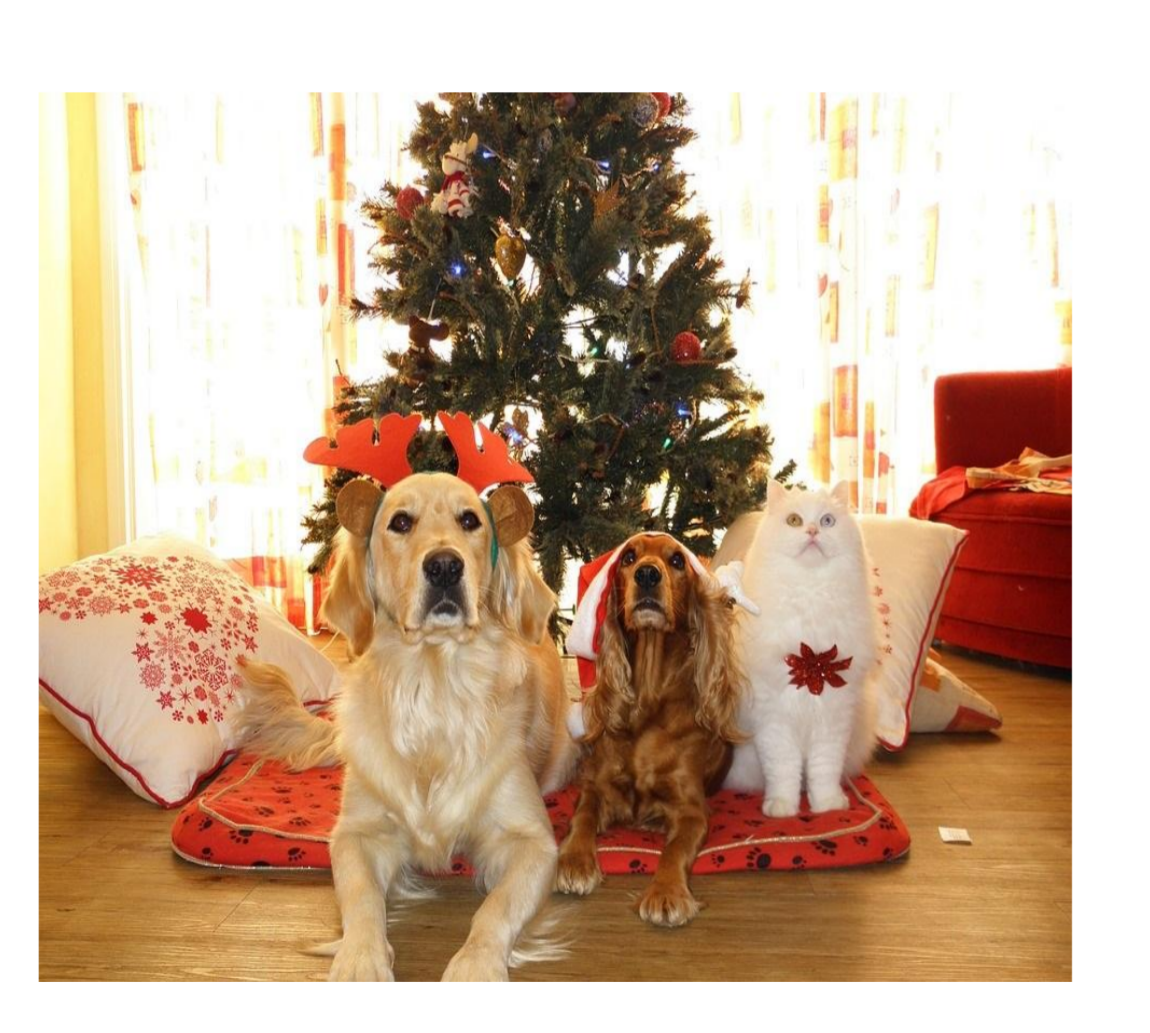
\includegraphics[width=7cm]{objectDetection/retall1.png}}
\subfigure[Divide image into grid.]{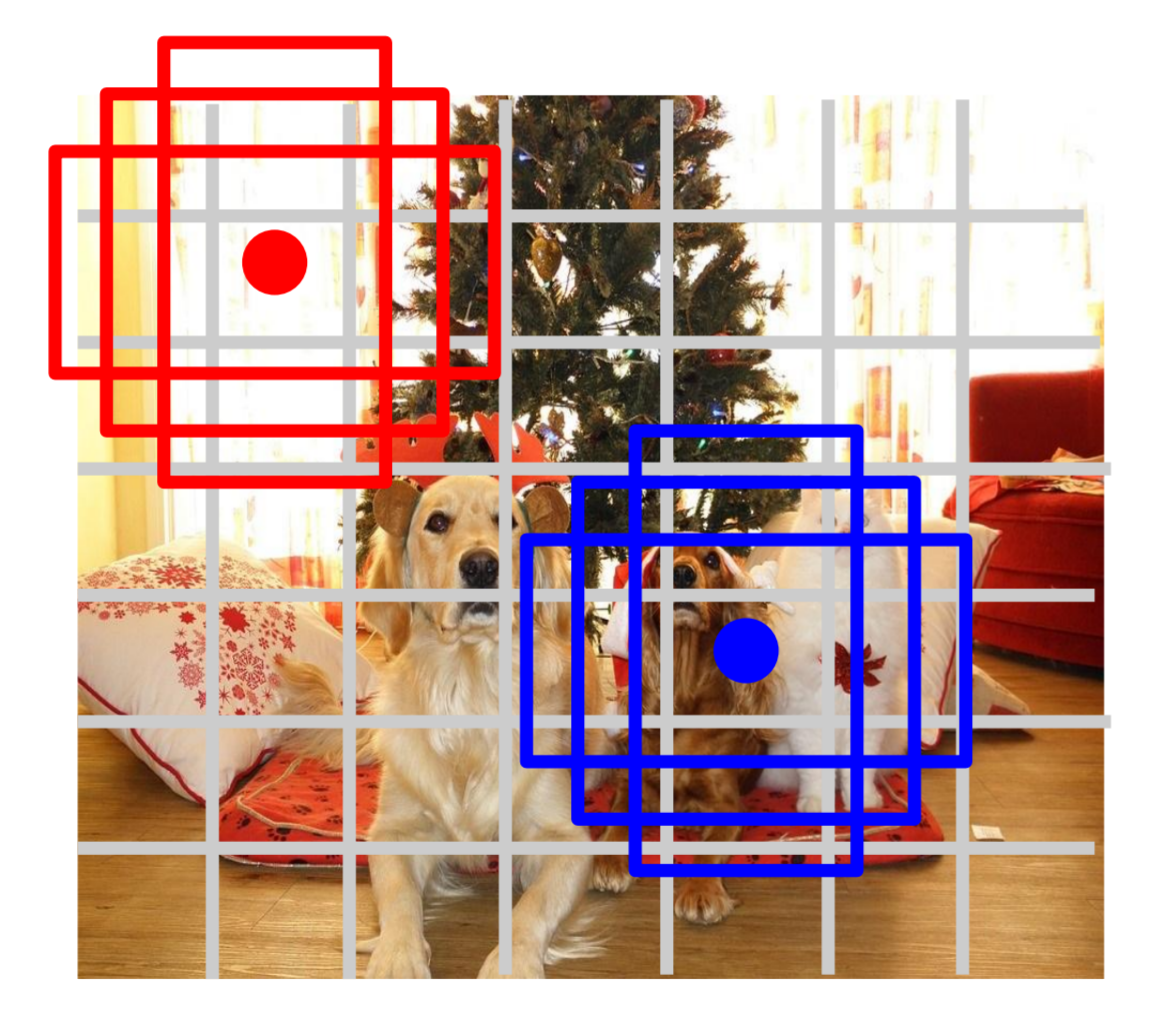
\includegraphics[width=7cm]{objectDetection/retall2.png}}\\


\caption{SSD detector scheme.}
\label{yolo1}
\end{figure}


\begin{figure}[H]
\centering         
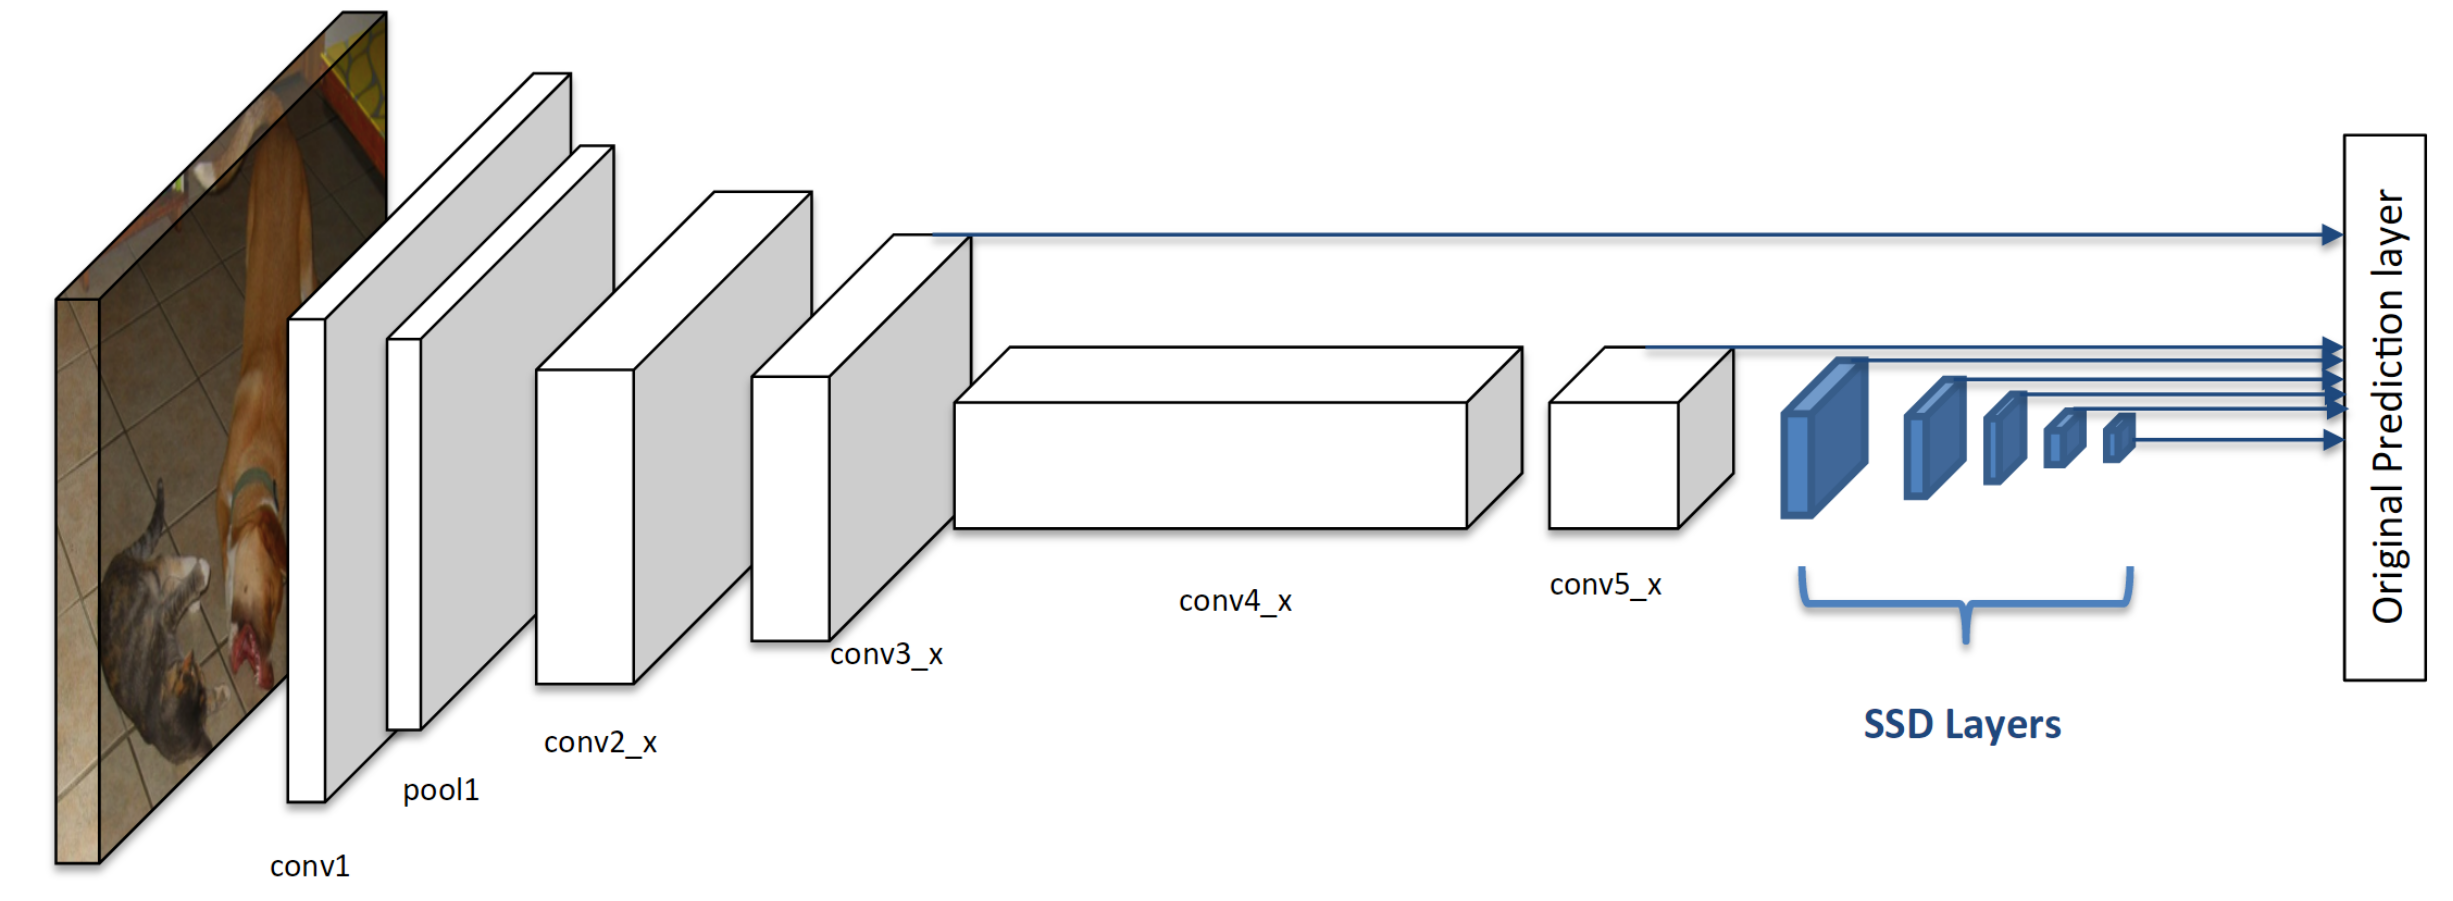
\includegraphics[width=12cm]{objectDetection/ssdArchitecture2.png}
\caption{SSD architecture.} \label{yolo2}
\end{figure}



\item RFCN \cite{rfcn}, it stands for Region-based fully convolutional network and it was developed by the same authors of SSD. They noticed the lacks of the SSD, the SSD algorithm computes the object detector on the feature map, and at this level the features have a low spatial resolution, this involves do not detect small objects. So the authors inspired by the fully convolutional architectures, upsample those feature maps and compute the object detector like the SSD algorithm.

\end{itemize}



In the survey \cite{cnnComparision}, they compared the different methods including changing the features extractors ( ResNet, Inception, VGG ) and they measured the precision ( mean average precision ) and computing time. This results are showed in \ref{comparisio}. The conclusion are as follows, SSD is the fastest detector, RFCN it has the best balance between speed-accuracy, and FasterRCNN, is the most accurate detector although is slower than the other ones.



\begin{figure}[H]
\centering         
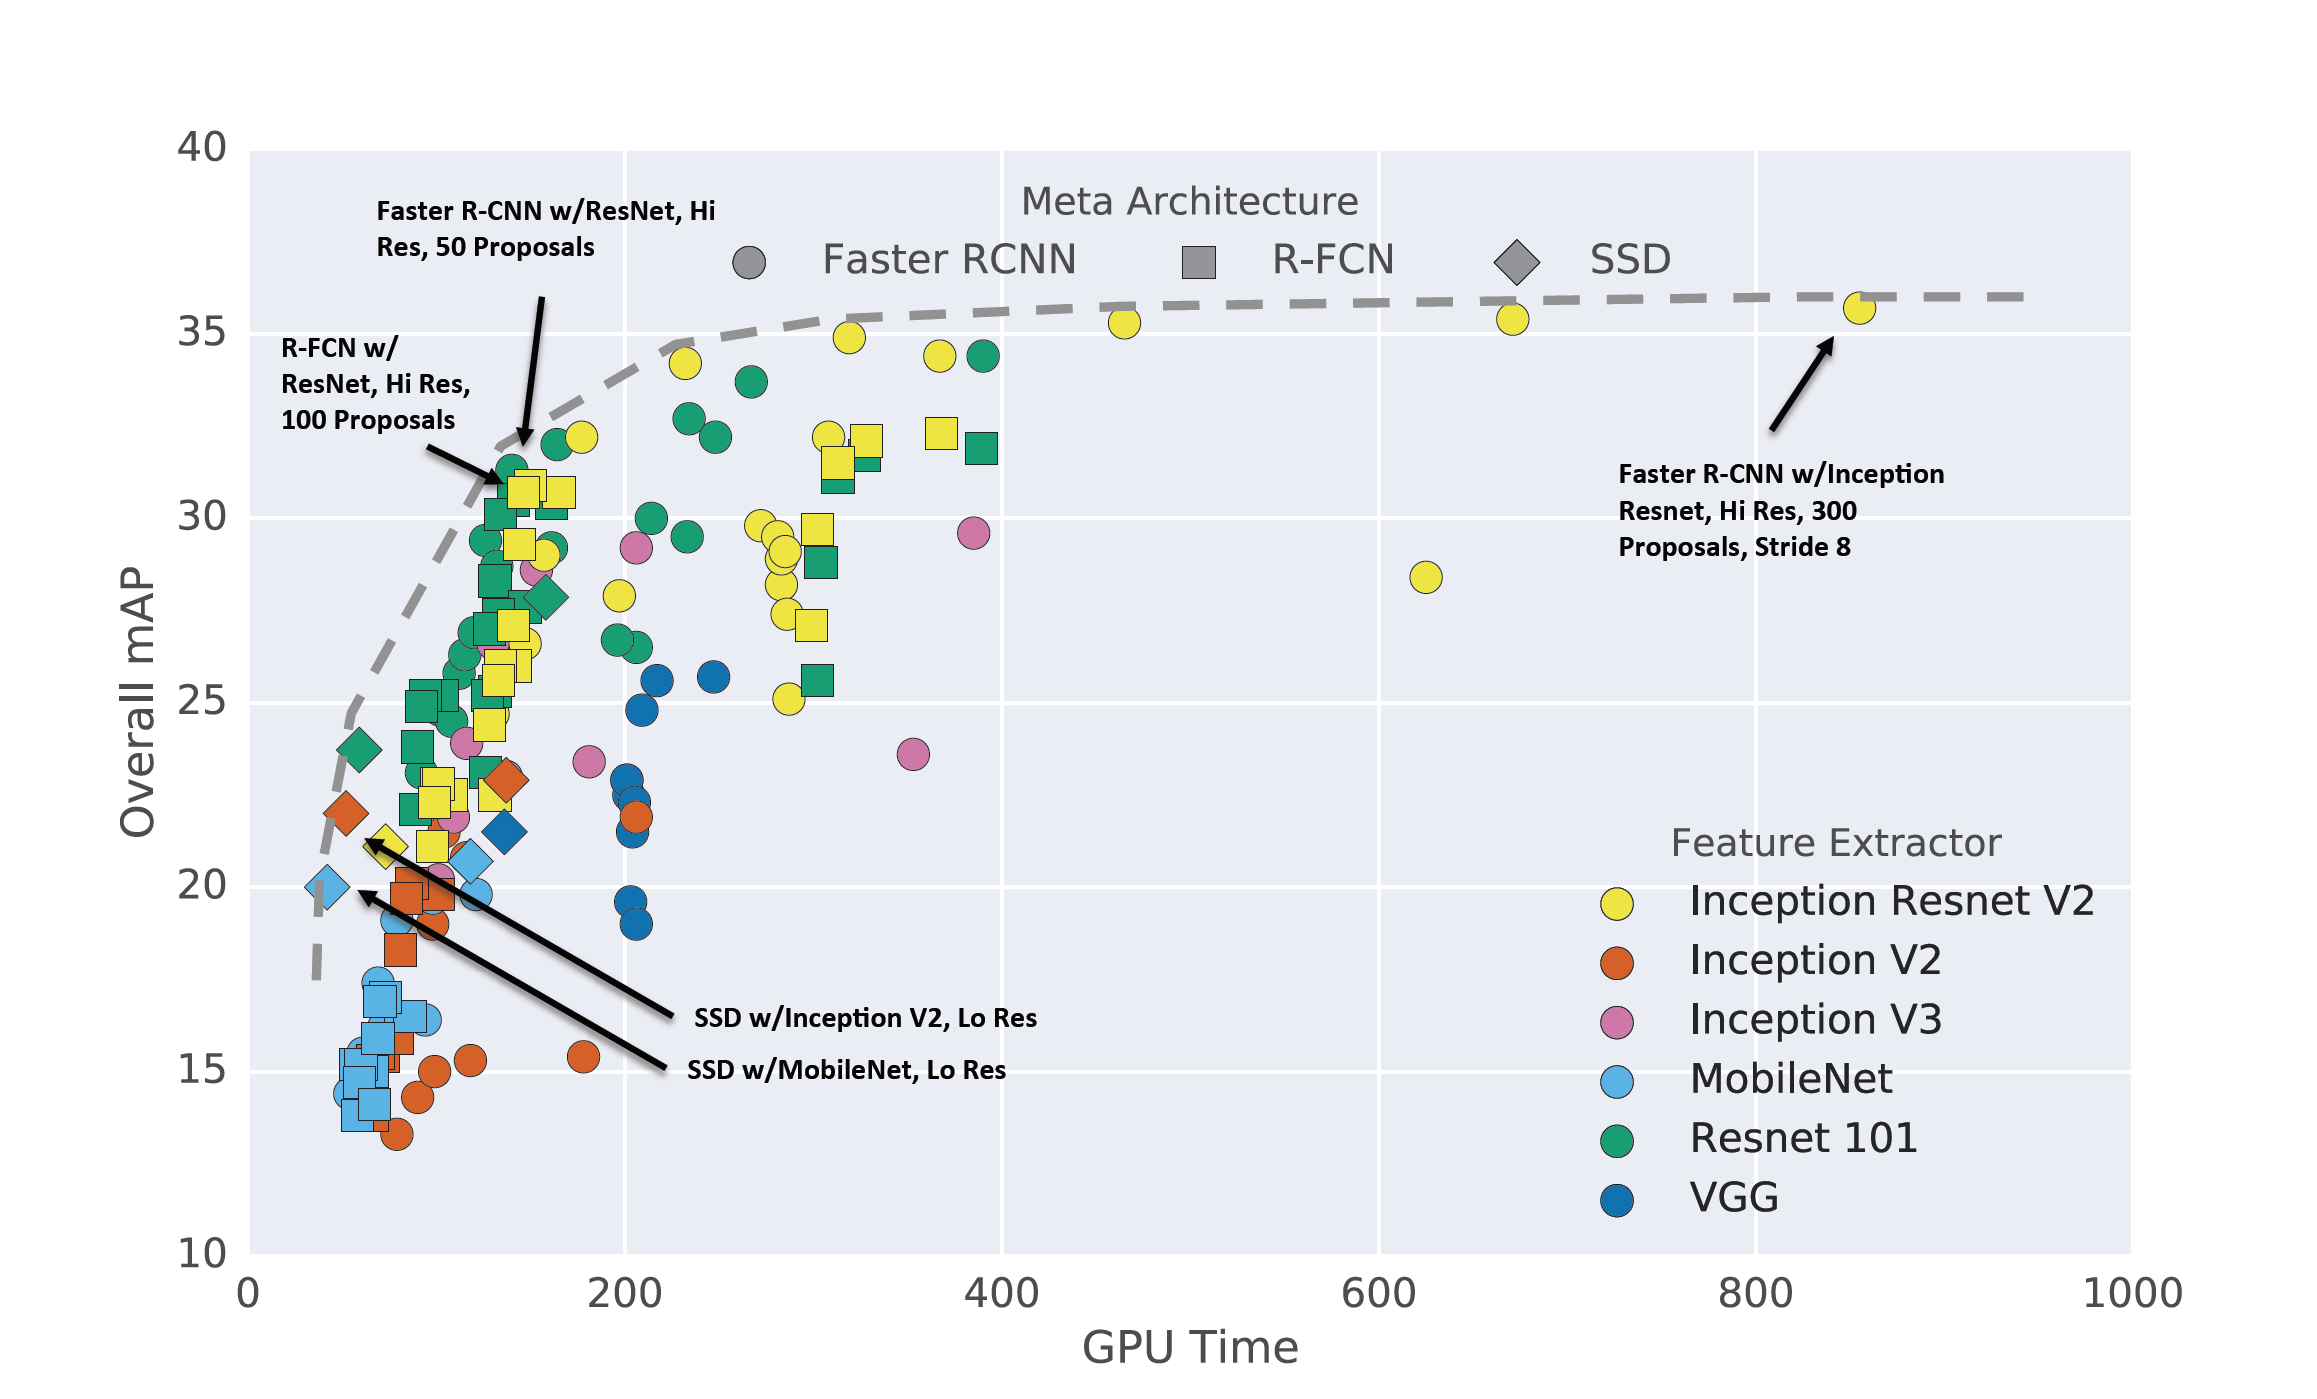
\includegraphics[width=0.9\linewidth]{objectDetection/comparisionTensor.png}
\caption{Comparison architectures.} \label{comparisio}
\end{figure}

We will finish off our review with a numeric comparison of the methods, as we can observe in the table \ref{tableDet}. This information is extracted from the original papers with their implementation, all of them are trained with the union of the training set of VOC07, VOC12, and COCO, and subsequently evaluate on VOC07 test set on a Nvidia Titan X GPU. These results give us an intuition on which detector will be suitable for our task.

\begin{table}[H]
\centering

\begin{tabular}{lllll}
                    & \textbf{mAP} & \textbf{mAP\_person} & \textbf{FPS} & \textbf{Proposals} \\
\textit{RCNN}       & 66           & 64.2                 & 0.077        & 2000               \\
\textit{FastRCNN}   & 70           & 69.9                 & 6.7          & 2000               \\
\textit{FasterRCNN} & 85.6         & 82.3                 & 7            & 6000               \\
\textit{SSD300}     & 81.2         & 81.4                 & 46           & 8732               \\
\textit{SSD512}     & 83.2         & 84.6                 & 19           & 24564              \\
\textit{YOLO}       & 66.4         & 63.5                 & 45           & 98                 \\
\textit{YOLOv2}     & 78.6         & 81.3                 & 40           & -                  \\
\textit{RFCN}       & 83.6         & -                    & 10           & -                  \\
\textit{PVANET}     & 84.9         & -                    & 31.3         & 300               
\end{tabular}

\caption{Summarize of the object detectors.}
\label{tableDet}
\end{table}


\subsection{Feature tracking}


\subsubsection{Features}\label{feature}

Our goal is to find points in an image, that can be found in other images and then compute some information, in this case, the movement. The characteristics of good features are:

\begin{itemize}

\item Repeatability, the same feature can be found in several images despite geometric and photometric transformations.

\item Matchability, each feature has a distinctive description, thus easy to find.

\item Efficiency, few features have to compact much more possible information.

\item Locality, a feature occupies a relatively small area of the image, so therefore it is robust to clutter and occlusion.

\item Performance, computation speed of features is a critical parameter. 

\end{itemize}

Features points are used in all sort of operations in computer vision: Image alignment, 3D reconstruction, Motion Tracking, Object recognition, Index database retrieval, robot navigation and so on.

Looking at the figure \ref{patches}, the flat patch, is a patch without texture and impossible to localize. Patches with large contrast edges are easier to localize, although straight lines segments at a single orientation suffer from the \textit{aperture problem}, are also impossible to localize. Finally, patches with large gradients in at least two different orientations are the easiest to localize.

\begin{figure}[H]
		
\centering

\subfigure[Flat region.]{
\includegraphics[width=5cm]{lucasKanade/flat.png}}
\subfigure[Edge region.]{
\includegraphics[width=5cm]{lucasKanade/edge.png}}
\subfigure[Corner region.]{
\includegraphics[width=5cm]{lucasKanade/corner.png}}\\


\caption{Types of patches.}
\label{patches}
\end{figure}

These intuitions can be formalized by looking at the simples possible matching criterion for comparing two images patches, their weighted summed square difference:

%Change in appearance for the shift [u,v]:

%$$ E(u,v) = \sum_{x,y} w(x,y) [I(x+u,y+v)-I(x,y)]^{2}$$
$$ E(u) = \sum_{i} w(x_{i}) [I(x_{i}+u)-I(x_{i})]^{2}$$

where $I(x)$ is the image, $I(x+u)$ is the shifted image, and $w(x,y)$ is a window function like a box or gaussian kernel around the pixel, and the summation $i$ is over all the pixels in the patch. Then we are looking for points, which if we move according to $u$ we have a change. 



When performing feature detection, we do not know which other image locations the feature will end up being matched against. Therefore, we can only compute how stable this metric is with respect to small variations in positions $\Delta u$ by comparing an image patch against itself:

$$ E( \Delta u) = \sum_{i} w(x_{i}) [I(x_{i}+\Delta u)-I(x_{i})]^{2}$$

Using a Taylor series expansion of the image function $I(x_{i}+\Delta u) \approx I(x_{i}) + \nabla I(x_{i})*\Delta u  $ we can approximate the expression as follows:

$$ E( \Delta u) \approx \sum_{i} w(x_{i}) [I(x_{i})+\nabla I(x_{i}) \Delta u-I(x_{i})]^{2}$$


$$ E( \Delta u) = \sum_{i} w(x_{i}) [\nabla I(x_{i}) \Delta u]^{2}$$

With algebraic notation it transforms to:

$$ E( \Delta u) = \Delta u^{T} M \Delta u$$

where $ \nabla I(x_{i}) = [I_{x},I_{y}](x_{i}) $ is the image gradient and $M$ is the second moment matrix:

\[ M = \left( \begin{array}{ccc}
I_{x}^{2} & I_{xy}^{2} \\
I_{xy}^{2} & I_{y}^{2} \end{array} \right).\] 

Computing the eigenvalue decomposition of this matrix, shows the directions of the fastest change, thus a measure of the \textit{cornernes}. There are several algorithms that use in different ways this eigenvalues:

%In the figure \ref{corner} we can observe the relationship between eigenvalues and patches types.
%
%
%
%
%\begin{figure}[H]
%\centering         
%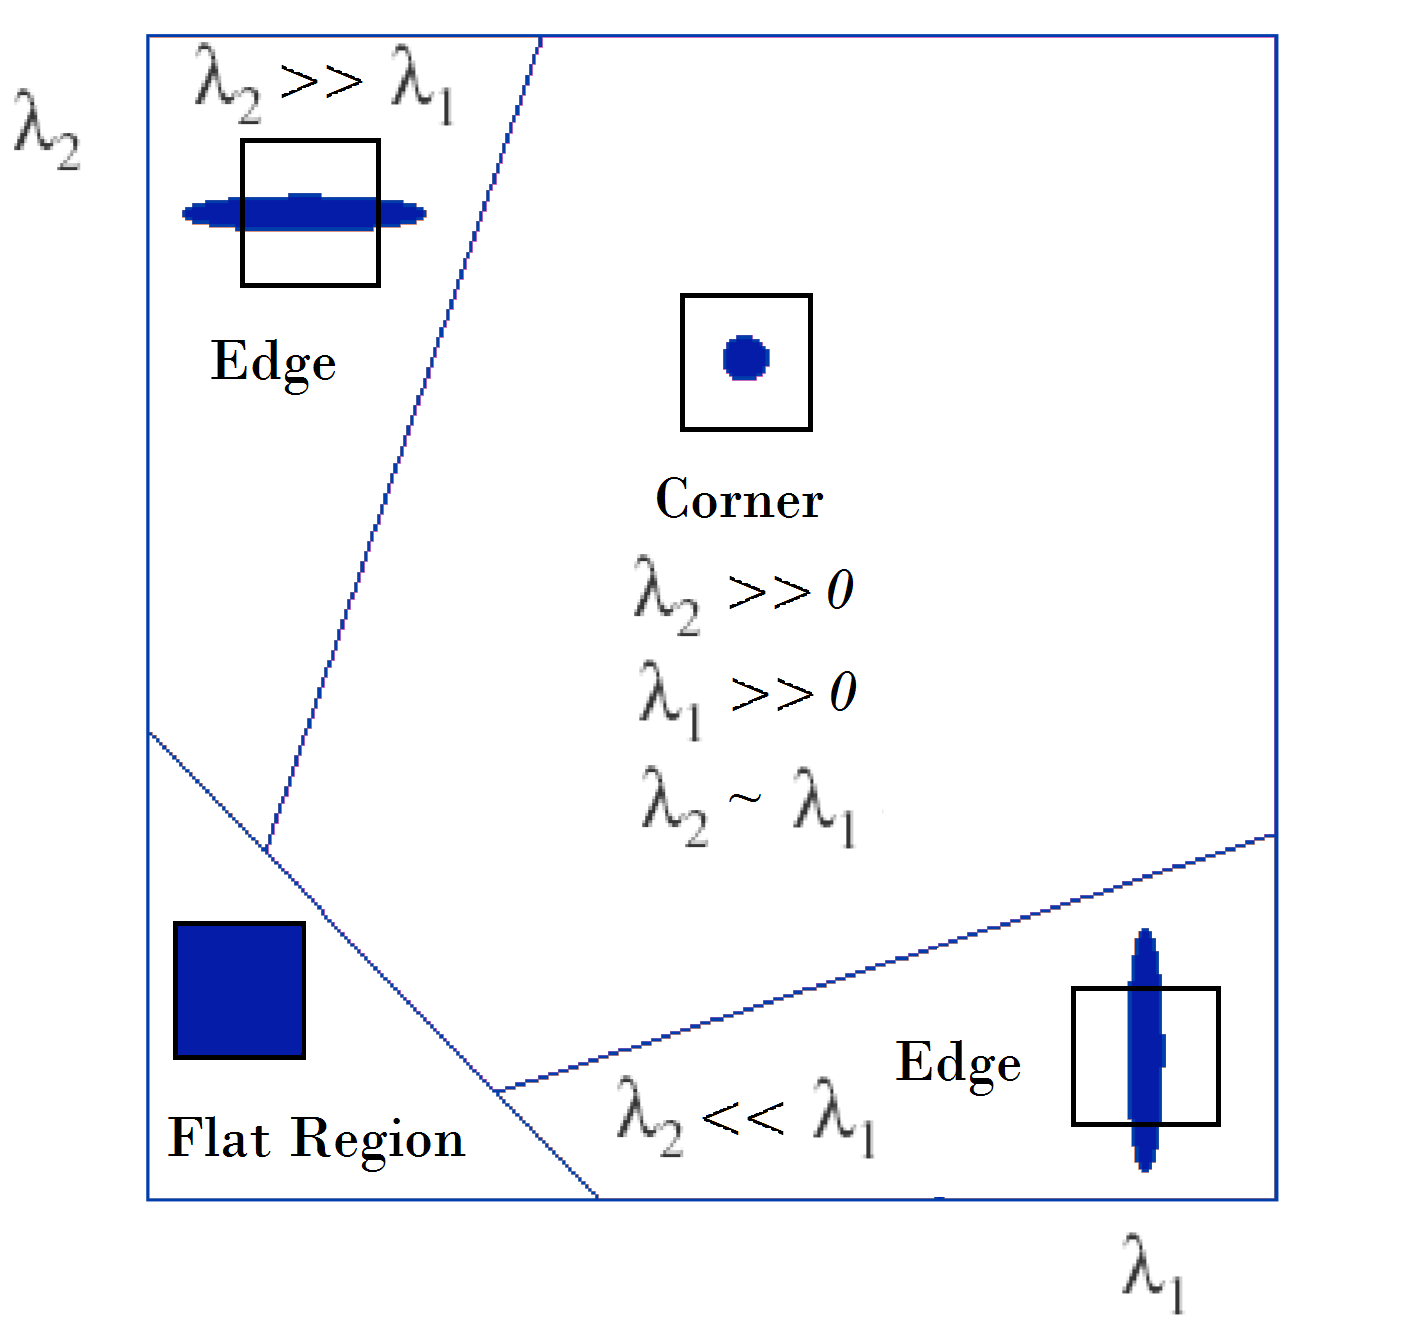
\includegraphics[width=0.6\linewidth]{lucasKanade/harrisMillora.png}
%\caption{Eigenvalues response for different regions .} \label{corner}
%\end{figure}




%There are several algorithms that use in different ways this eigenvalues:

\begin{itemize}

\item Harris \cite{harris}, they propose a corner detection response function. So for each pixel, they compute a matrix $M$ and with it, they compute the function
R, $R = det(M)-a \hspace{0.1cm} trace^{2}(M)$. if R is large, that pixel is a corner, if R is negative with larger magnitude, it is a an edge, and if R is small it is a 
flat region. So the they a threshold to classify those pixels as a corner. 

\item Shi-Tomasi \cite{shi}, they define the \textit{cornerness} in another way. The image has a maximum value ( e.g. 255), so $\lambda_{1}$, $\lambda_{2}$ also have an upper bound, then it is only necessary to check that $min(\lambda_{1},\lambda_{2})$ is large enough, this is how they define \textit{cornerness}. This feature is called good features to track, because the authors defined a \textit{good} features those whose motion can be estimated reliably, and they reached the same conclusions as Harris. This method is implement in the OpenCV's routine \texttt{goodFeaturesToTrack()}.

\end{itemize}

\subsubsection{Motion estimation}

Now, we have invariant points, we want to estimate the motion of those points. In order to do so, we compute the optical flow. This is the apparent two-dimensional motion of brightness pattern in the image. In the next figure \ref{refArchiteOF} we visualized this idea.


\begin{figure}[H]
		
\centering

\subfigure[$I(x,y,t) $.]{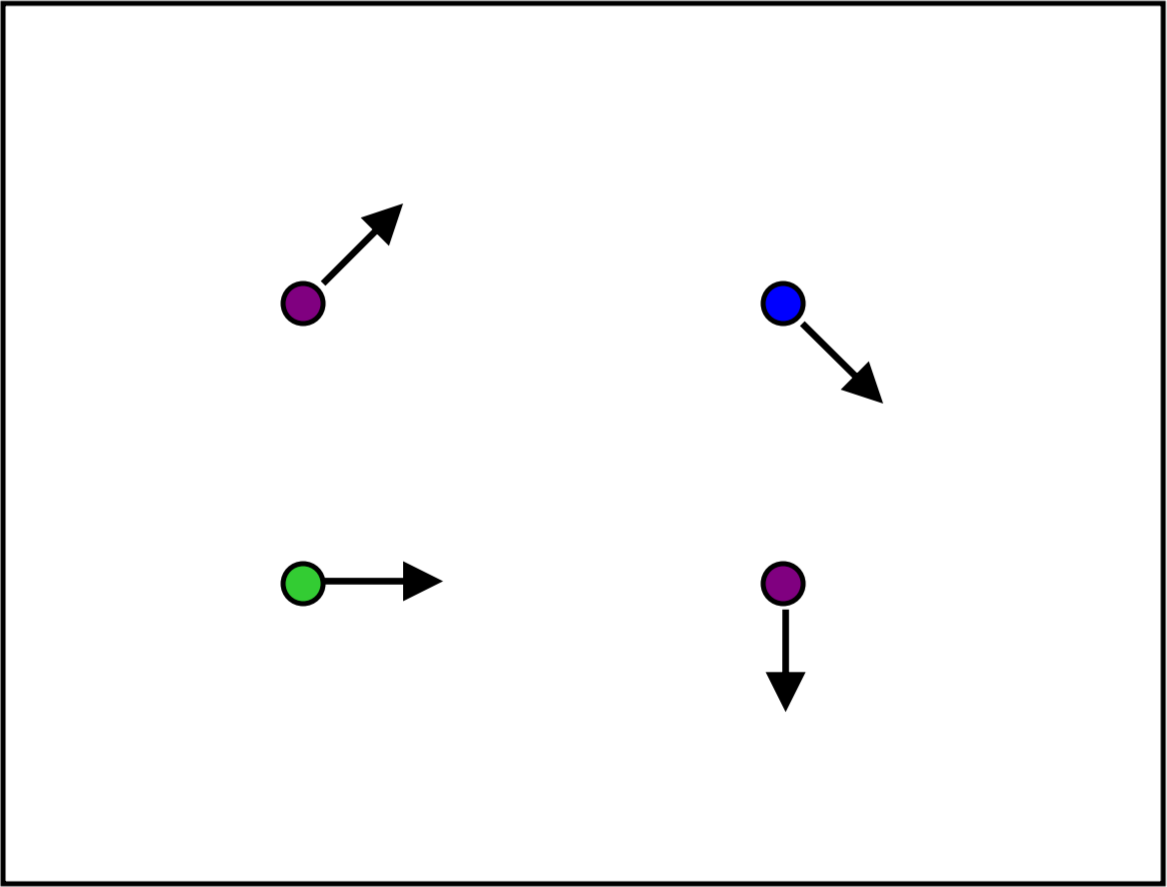
\includegraphics[width=5cm]{lucasKanade/retall1g.png}}
\subfigure[$I(x,y,t+1) $.]{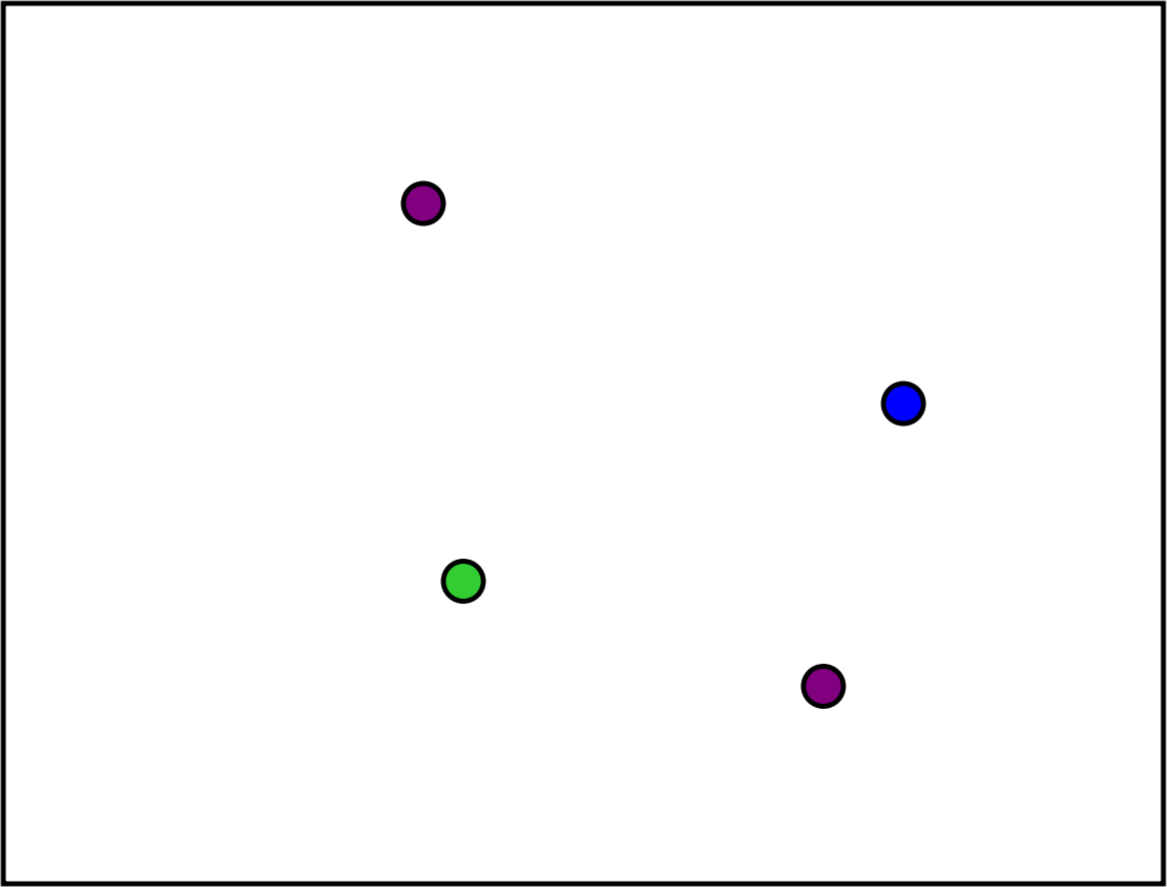
\includegraphics[width=5cm]{lucasKanade/retall2g.png}}\\


\caption{Optical flow example.}
\label{refArchiteOF}
\end{figure}

So, the question is: How do we estimate pixel motion from image $I(x,y,t)$ to image $I(x,y,t+1)$. We need to solve the pixel correspondence problem. Given a pixel in $I(x,y,t)$, look for nearby pixels of the same color in $I(x,y,t+1)$. Solving this problem is what is referred as the optical flow problem. By nearby pixels and same colour we have two assumptions:

\begin{itemize}

\item Colour constancy: a point in $I(x,y,t)$ looks the same in $I(x',y',t+1)$. For grayscale images, this is called \textit{Brightness constancy constraint}. Stated in mathematical formulation:

$$ I(x,y,t) = I(x+u,y+v,t+1) $$

$$ 0 = I(x+u,y+v,t+1)-I(x,y,t)  $$

\item Small motion: Subsequent points do not move very far, so we can estimate the motion by Taylor expansion: 

$$ I(x+u,y+v) 	\approx  I(x,y) + \dfrac{ \partial I}{\partial x}u +\dfrac{ \partial I}{\partial y}v + higher \hspace{0.1cm} order \hspace{0.1cm} terms $$


\end{itemize}
 
Then, combining these two equations, we get:

$$ 0 	\approx  I(x,y,t+1) + I_{x}u +I_{y}v - I(x,y,t) $$

where $I_{x} =  \dfrac{ \partial I}{\partial x}$, isolating the terms we obtain:

$$ 0 	\approx [I(x,y,t+1) - I(x,y,t)] + I_{x}u +I_{y}v $$

$$ 0 	\approx I_{t} + I_{x}u +I_{y}v $$

In the limit of $t$, $u$ and $v$ approaches zero ( assumption of small motion ), so it becomes, what it is called the the \textit{brightness constancy constraint equation}:
$$ 0 	= I_{t} + I_{x}u +I_{y}v $$

If we look closely, we realized that we have two unknowns $u,v$ and one equation. This is an underdetermined system. Intuitively, this means, that locally we can only determine the component of the flow in the gradient direction, the component of the flow parallel to an edge is unknown, this is the called the aperture problem. To recover the motion we need to add some extra constraints. There are several types of constraints to solve this problem:

\begin{itemize}

\item \textbf{Global constraint}, adding a smooth constraint to the brightness constraint, this new constraints penalizes for changes in $u$ and $v$ over the images, it assumes that the motion fields vary smoothly over the image. This approach was developed by Horn and Schunk \cite{horn}.

\item \textbf{Local constraint}, locally the motion field is almost the same, so we add the neighbours pixels to the equation. This approach was developed by Lucas and Kanade \cite{LucasKana}.
\end{itemize}



\textbf{Local constraint}

In this thesis we use the Local constraint to solve the optical flow problem. As we stated above, we add a local constraint to get more equations, this assumes that the motion field is the same in the locality. From the brightness constraint equation:

$$ 0 = I_{t}(p_{i}) + \nabla I(p_{i}) \hspace{0.1cm} [u \hspace{0.2cm} v]$$

Adding the neighborhood equations:

% 2

\[
\begin{bmatrix}
    I_{x}(p_{1}) & I_{y}(p_{1})  \\
    I_{x}(p_{2}) & I_{y}(p_{2})  \\
    \vdots & \vdots  \\
    I_{x}(p_{n}) & I_{y}(p_{n})
\end{bmatrix}
\begin{bmatrix}
    u \\
    v \\
\end{bmatrix}
=
\begin{bmatrix}
    -I_{t}(p_{1}) \\
    \vdots \\
    -I_{t}(p_{n}) \\
\end{bmatrix}
\]


Now, there are more equation than unknows, it is an overdetermined system, we have to solve it with the least squares technique. It is based on the optimization of the function:
%by using the pseudo inverse:
% 4
$$(A^{T}A) \hspace{0.1cm} d=A^{T} \hspace{0.1cm} b$$

Using the image notation:

% 5

\[
\begin{bmatrix}
    \sum I_{x}I_{x} & \sum I_{y}I_{x}  \\
    \sum I_{x}I_{y} & \sum I_{y}I_{y}   \\
\end{bmatrix}
\begin{bmatrix}
    u \\
    v \\
\end{bmatrix}
=
\begin{bmatrix}
    - \sum I_{x}I_{t} \\
    - \sum I_{y}I_{t} \\
\end{bmatrix}
\]



The system has a solution when $A^{t}A$ is invertible, it will be invertible when is well conditioned, this is when the ratio of the great and the small eigenvalues of the matrix is large but no too much. The matrix $A^{t}A$ in terms of image formulation is the second order matrix that we stated in the section \ref{feature} developing the \textit{cornerness}, then in order to be solvable it should have a strong gradient in both directions. After checking the invertability, we can solve the problem and extract the motion field:

% 6
$$ d = (A^{T}A)^{-1} \hspace{0.1cm}  A^{T}  \hspace{0.1cm} b  $$

Thus, using the image notation:

\[
\begin{bmatrix}
    u \\
    v \\
\end{bmatrix}
=
\begin{bmatrix}
    \sum I_{x}^{2} & \sum I_{y}I_{x}  \\
    \sum I_{x}I_{y} & \sum I_{y}^{2}   \\
\end{bmatrix}^{-1}
\begin{bmatrix}
    - \sum I_{x}I_{t} \\
    - \sum I_{y}I_{t} \\
\end{bmatrix}
\]



In practice motion is large, the assumption that it is small fails, consequently the approach using Taylor expansions. For two reasons, the linearity does not hold, in order to solve it, we apply an iterative refinement, which consists in compute the displacement, apply it to the pixels, and compute it again till it converges. The other one is there are local minimum and it will fail into it. To solve it, we need to utilize a coarse to fine approach, the idea is to use multiresolution to compute optical flow, the basic is that in a low resolution image the motion between pixels is very small and we can compute optical flow.

So, in order to do so, we use image pyramids, this consists in downsample these images to specific resolution, then in top level, we compute the motion field using the previous stated method, then 
we upsample the motion field and the images, We apply a transformation to one image according to the motion field computed in the previous level and then compute the optical flow between that 
transformed image and the other image, we apply this algorithm in all the resolutions

% image pyramids


\begin{figure}[H]
\centering         
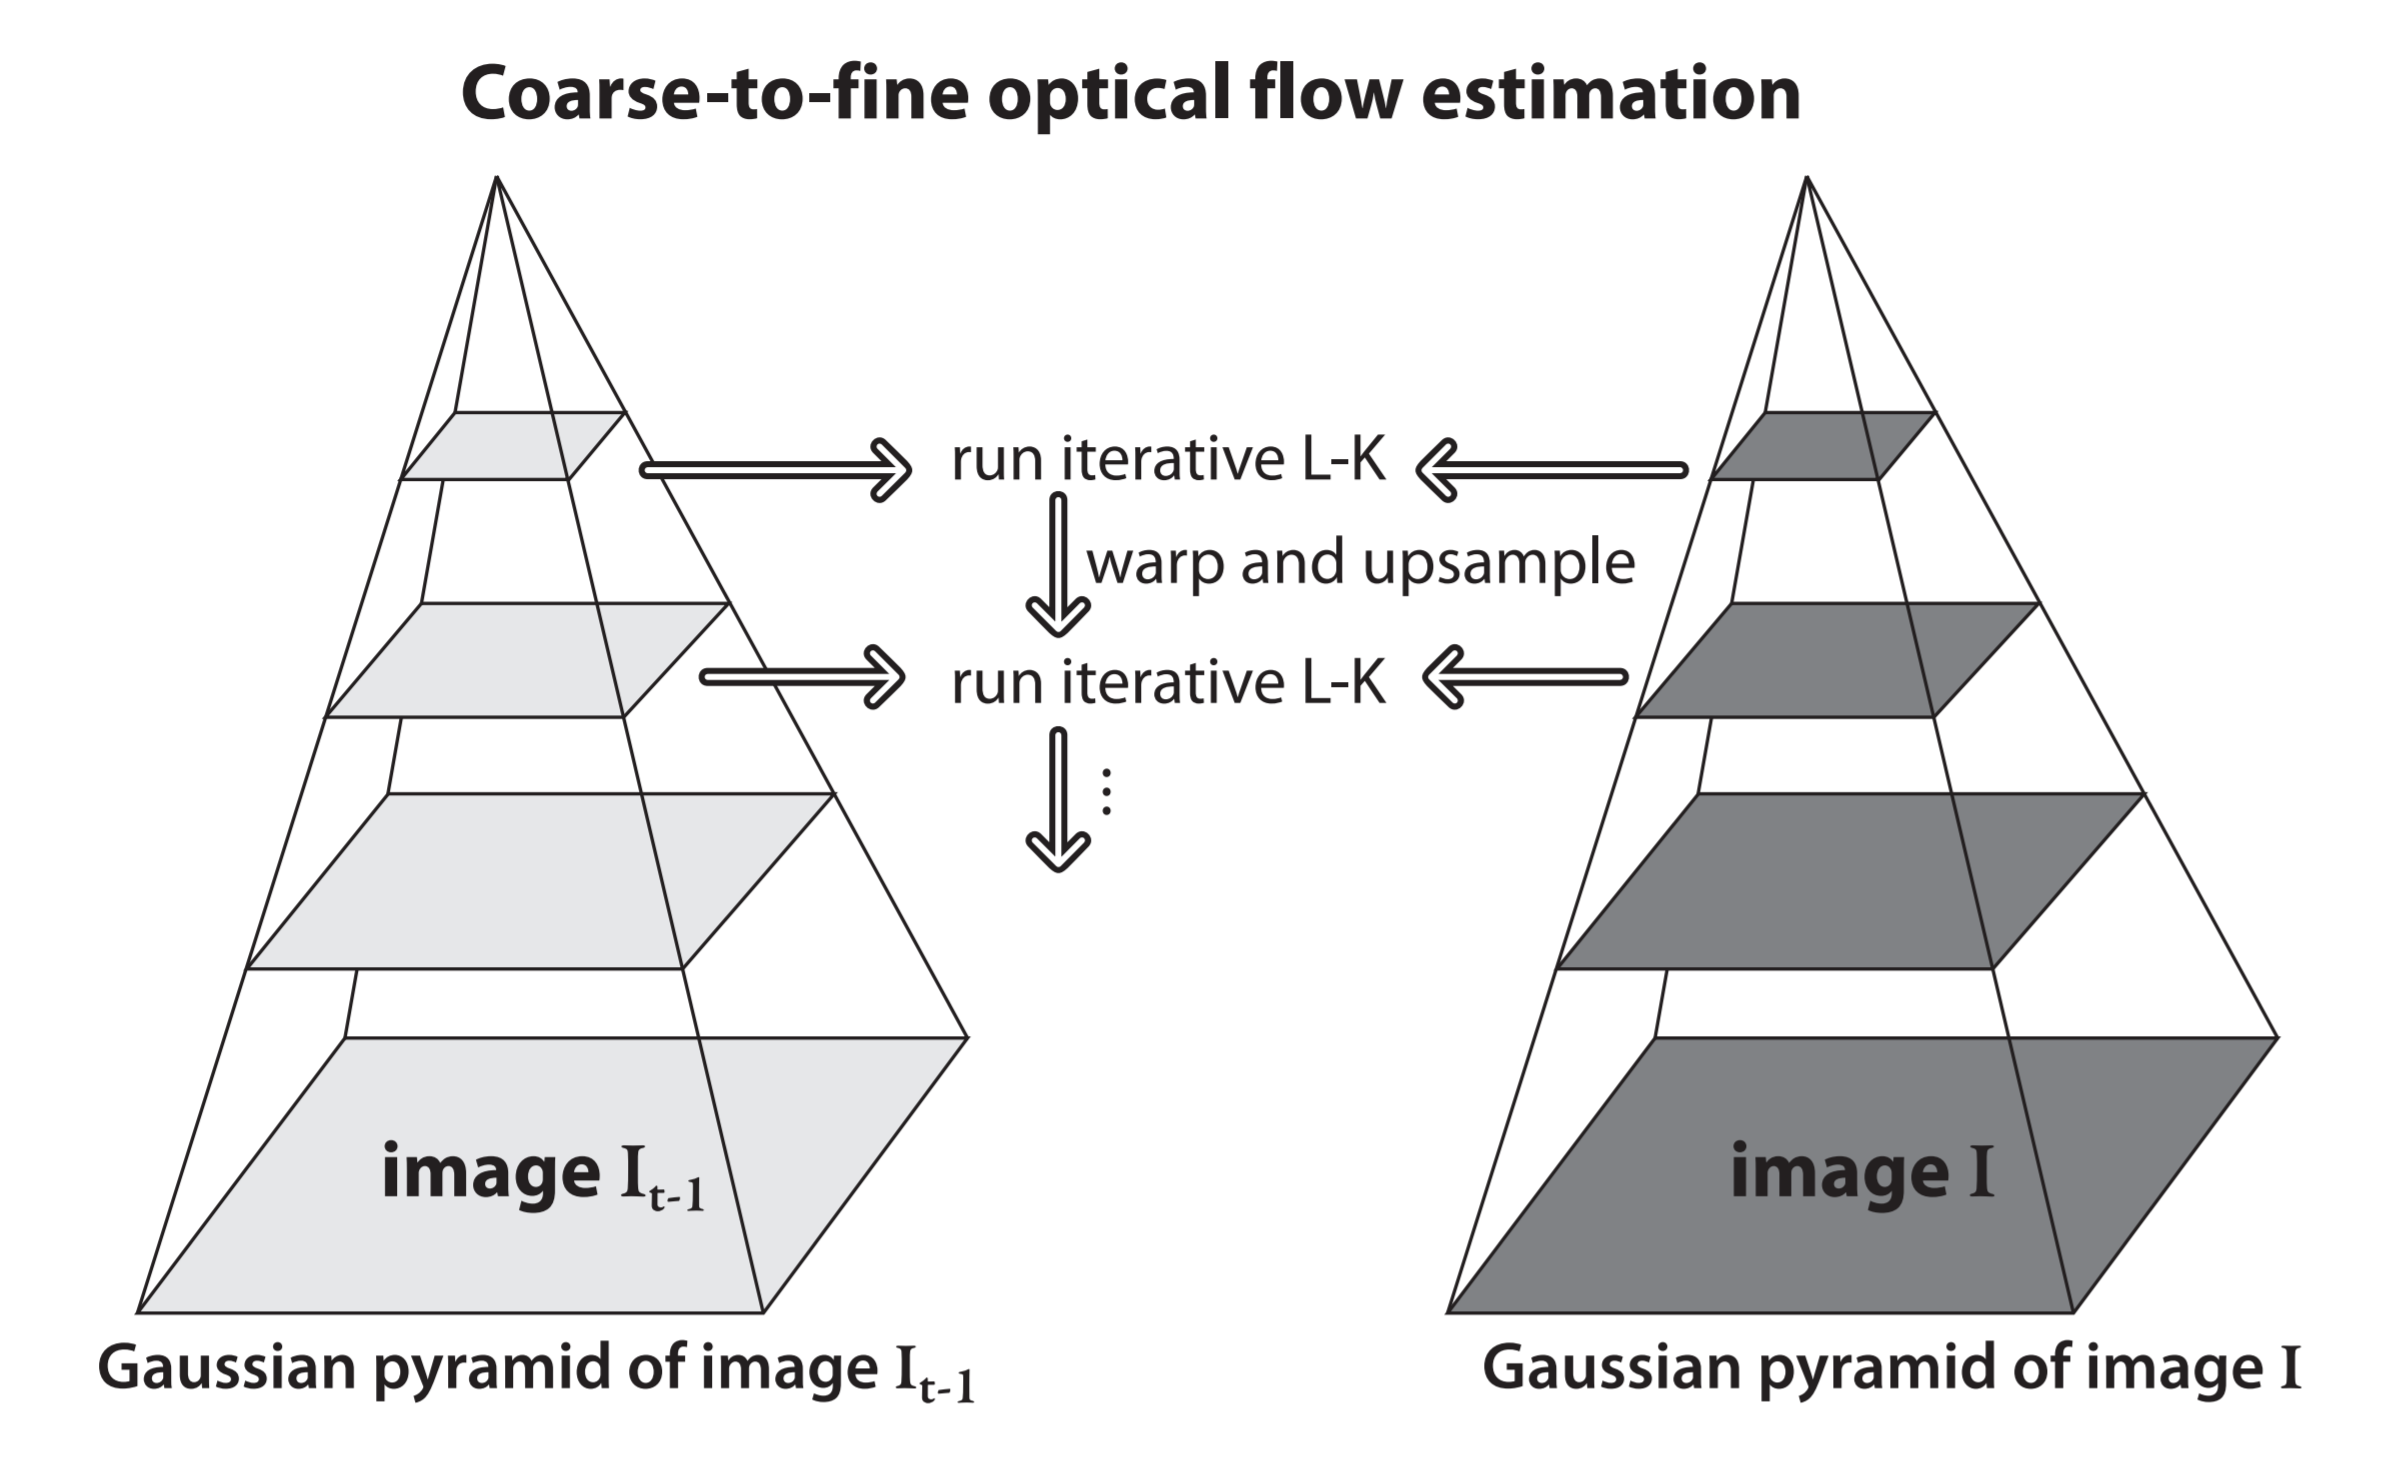
\includegraphics[width=0.6\linewidth]{lucasKanade/piram.png}
\caption{Optical flow with pyramids.} \label{corner}
\end{figure}





\section{Person re-Identification}\label{misMatch}


After running the tracking module we might lose some trackets and in the detection step we might recover them. We need a module to check whether these have the same identity. In order to do so, we studied the methods to recover the identity with deep learning techniques.

Person identification is thoroughly studied in the field of Biometrics, it consists of  knowing one biometric characteristic, and comparing with a claiming identity query. Specifically, the topic of pedestrian identification based on images has raised in the last years, this is due to the growth of surveillance applications. Also inside the topic of tracking there is a subfield called data association which studies this problem, it consists in matching trackets with further pedestrian detections.

Let's define mathematical the problem, consider $G$ is a gallery composed of $N$ images, denoted as $(g_{i})_{i=1}^{N}$. They belong to $N$ different identities $ 1,2,...,N $. Given a query image $q$, its identity is determined by:

%$$ i^{*} = argmax_{i \in 1,2,...,Ni \in 1,2,...,N} \hspace{0.5cm} sim(q,g_{i})$$

$$ i^{*} = \underset{i \in 1,2,...,N}{\arg\max} \hspace{0.5cm} sim(q,g_{i}) $$

where $i^{*}$ is the identity of probe $q$, and $sim( . , . )$ is some kind of similarity function. There are several categories of this similarity function \cite{pastPresent}:

\begin{itemize}
 
\item \textbf{Hand-crafted systems}. This involves two components, an image descriptor and a distance metric algorithm. The most common image descriptors are those used in computer vision too, like colour \cite{lbp}, texture \cite{pairwise}, SIFT \cite{sift}, bag of word \cite{bagword}. The general idea of distance metric learning is to keep all the vectors of the same class closer while pushing vectors of different classes further apart. The most commonly used formulation is based on the class of Mahalanobis distance function \cite{kiisme}, \cite{lnnn}. Other works focus on learning discriminative subspaces \cite{lda}.

\item \textbf{Deep learning techniques}. Two types of CNN models are commonly employed in the community, the first is the classification model as used in image classification, the output is an identity label, and the second one is the siamese model using image pairs as input. The major drawback of the classification models is that they need a great quantity of training data by category, and most of the identifications datasets only provide a few examples for identity. So currently methods focus on siamese models.

\end{itemize} 

The main differences between them, is that in hand-crafted methods, feature representation of the data and the metric are not learned jointly, instead, deep learning techniques jointly optimize the representation of the input data conditioned on the \textit{similarity} measure being used \cite{EC1}. 





\subsection{Siamese networks}



The first work with siamese architectures were developed by LeCun \cite{siamLecun}, \cite{siameLecun2} and they addressed the identification of signatures, besides the siamese networks are used in a variety of problems like: image recovery \cite{siameseQuer}, feature descriptor \cite{siameDescri}, comparing patches \cite{patch1}, one shot learning \cite{siameseOne}, and learning visual similarity \cite{siamesSImi}. 

Siamese CNN topologies can be grouped under three main categories, depending on the point where the information from each input is combined:

\begin{itemize}

\item \textbf{Cost function}. Input patches are processed by two parallel branches featuring the same network structure and weights. Finally, the top layers of each branch are fed to a cost function.

\item \textbf{In-network}. The top layers of the parallel branches processing the two different inputs are concatenated and some more layers added on top of that.

\item \textbf{Joint data input}. The two input patches are stacked together forming a unified input to the CNN.

\end{itemize}

Graphical we can observe those differences in \ref{siamese2Data1}.
\begin{figure}[H]
		
\centering

\subfigure[Cost function.]{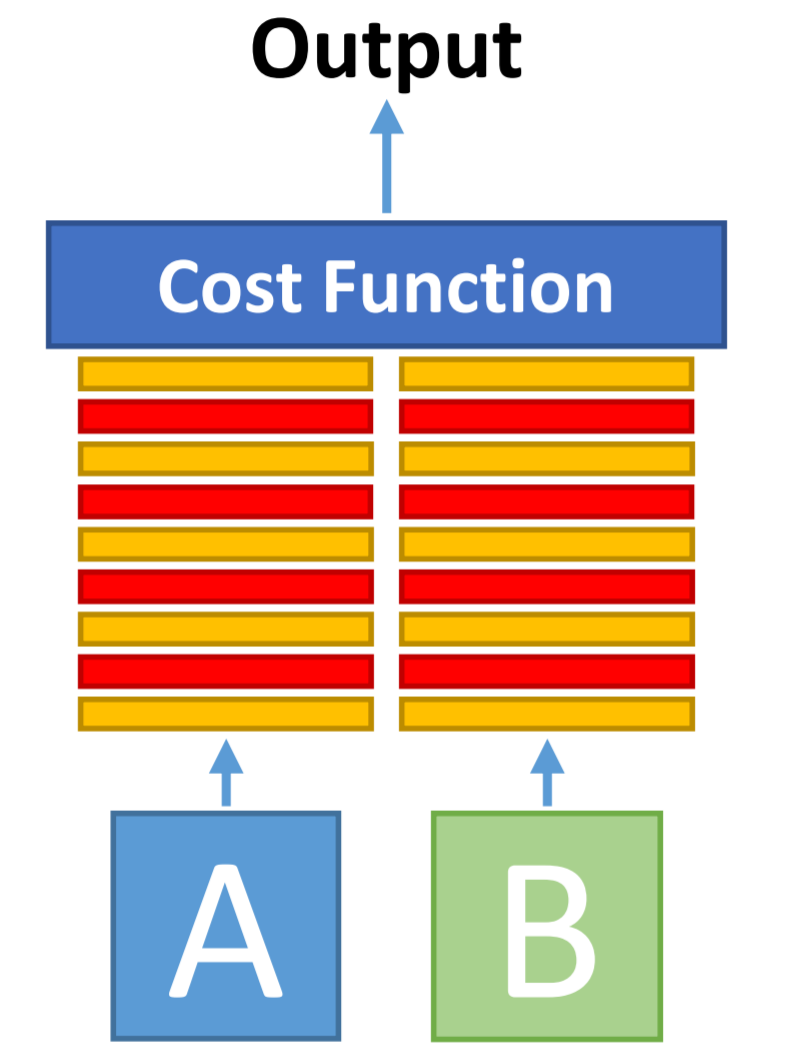
\includegraphics[width=2.7cm]{siamese/retall1.png}}
\subfigure[In-network.]{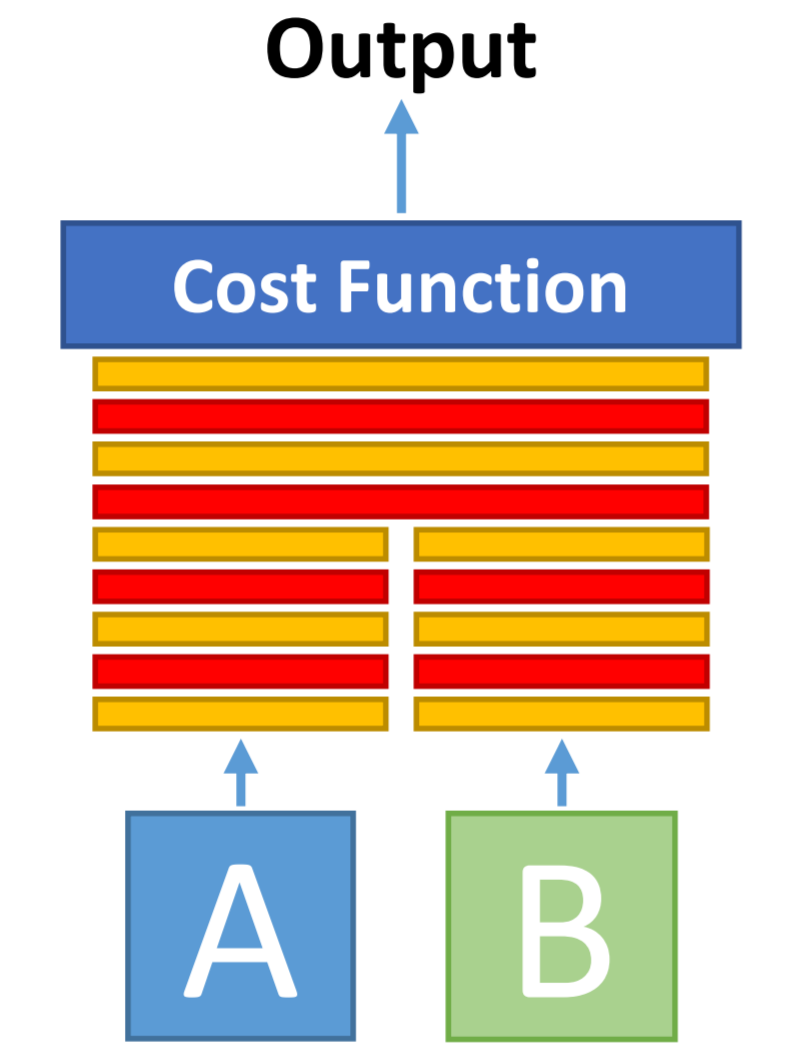
\includegraphics[width=2.7cm]{siamese/retall2.png}}
\subfigure[Joint data input.]{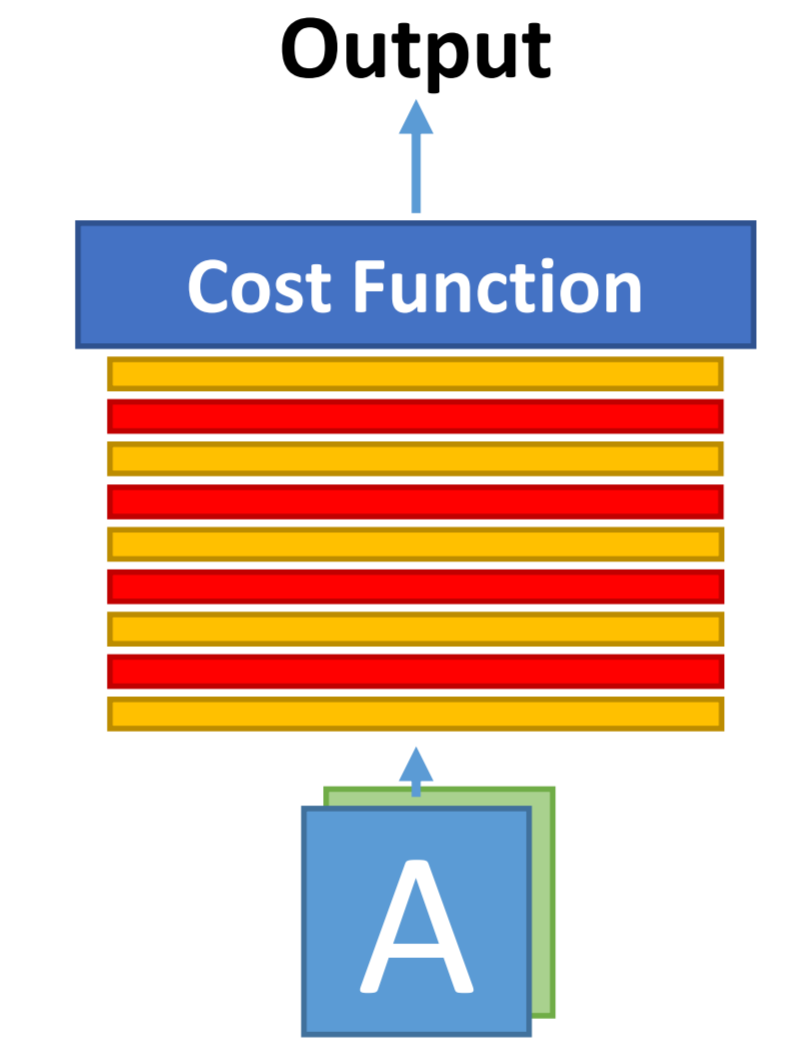
\includegraphics[width=2.7cm]{siamese/retall3.png}}

\caption{Siamese CNN topologies.}
\label{siamese2Data1}
\end{figure}


While the two first approaches have yield good results and historically were dominant, the best performance is obtained with the joint data input strategy. As pointed out by  \cite{patch1} and further corroborated by \cite{patch2}, and \cite{patch3}, jointly using information form both images from the first layer tends to deliver a better performance. 


In the field of person re-identification, the community has used these architectures, and they also, have developed their own loss function, what is called \textit{contrastive loss}, this loss is an extension of the Hinge loss of the SVM. This loss longs for getting close similar pairs and moving away according to one defined margin, dissimilar pairs. Although, the binary cross entropy is used by the community. Also, the community has focused in the developing of the datasets, increase the size and quality but there are not any landmark dataset.


There are several papers in the literature, one of the most famous is developed by Ahmed \cite{ahmed}, they used In-network architecture although in order to join to the convolutional layers, they used \textit{cross-input neighborhood differences} layer, this layer tried to increase the differences between the features of the inputs and obtain richer representation to the classification layer.

Another paper was published by Leal-Taixé \cite{lealTaixe}, they are also the authors of the MOT challenge, their network used a cost function architecture besides they used as inputs the two images and their optical flow. They used the network as part of a data association algorithm.




\lhead[]{CAPÍTULO \thechapter. Solution}
\chapter{Software implementation}\label{cap.software}

In this chapter, we explain the algorithm that we have designed for solving the visual people tracking problem and its software implementation. 

\section{System overview}

The main contribution of this work is to develope a tracking algorithm that utilizes neural network and do not miss the real time objective. To do so it uses the tracking-by-detection framework, it combines people detection using a neural network, somehow, slow but very accurate, and link these detections with feature tracking, very quick but prone to drift. 

The architecture of the system is summarized in the diagram \ref{software1}, it has a sequence of frames as input and a CSV file as output. This file has the structure of the MOT's evaluation software requires. We divided the computing in two threads, the object detector thread and the main thread. The first is responsible of given a frame compute their pedestrian detections and send them to the tracking thread, and the second one, the tracking thread, given a detection it computes the tracking procedure, in adition, when a new detection appears it combines with the tracker, this is called data association, and finally it saves the results of the algorithm.



\begin{figure}[H]
\centering         
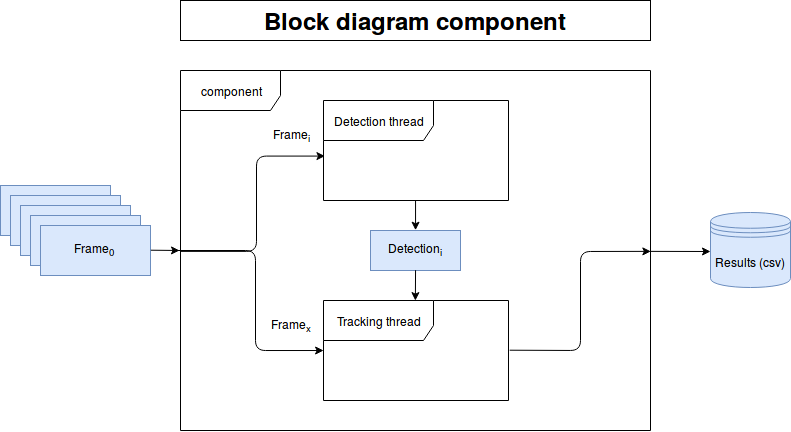
\includegraphics[width=8cm]{flows/bloque.png}
\caption{Block diagram of the component.} \label{software1}
\end{figure}


Temporally the system works as follows, when the algorithm starts, first of all it launches the object detector thread, it begins to compute the detections of the first frame. Meanwhile, the tracking thread remains idle, waiting for the detections. When the object detector finishes, it sends the detection to the tracking thread and at the same time starts to compute the detections of a predefined new frame. When the tracking thread has got a detection, it begins to compute the tracking between frames. Considering that the thread are not syncronized, the object detection thread goes ahead of the tracking thread it will have a detection whcih the tracking thread could not incorporate, thus, it saves the detections. When the tracking thread arrives to a frame that has a detection it has a mechanism to mix detection with trackets, what is called data association module, after running this module it will continue computing the tracking, when necessary it has a person re-identification module, to solve some possible identity incongruities. We can observe this temporal process in the next figure \ref{software2}, when $T$ represents a temporal step. When the object detector thread finishes computing all the detections it will \textit{die} and the tracking thread computes their task previously stated till it does not have any frame to process.


\begin{figure}[H]
\centering         
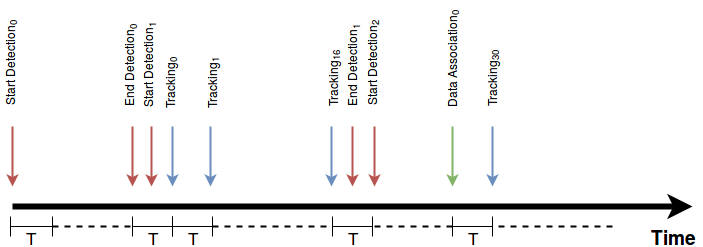
\includegraphics[width=14cm]{timesDiagram/timing.png}
\caption{Timing of the component.} \label{intro1}
\end{figure}


In the figure \ref{introTracking3} there is a flow chart of the algorithm and it summarizes as follows: The object detector thread reads images, processes the forward pass of the neural network and saves the detections in the shared buffer, it repeats this sequence until it has processed all the predefined list of frames. In another hand, the main tread, activates the object detector thread and waits till it gets the first detection, after this, it starts the tracking algorithm. It reads the images and computes the motion of all the regions of interest. However, at beginning of each cycle it checks whether it has newer detection to mix in. This is the main operating mode of the algorithm and it summarizes in the figure \ref{system1}. In the next sections we will develope in detail these parts. 

\begin{figure}[H]
	
\centering

\subfigure[Main thread.]{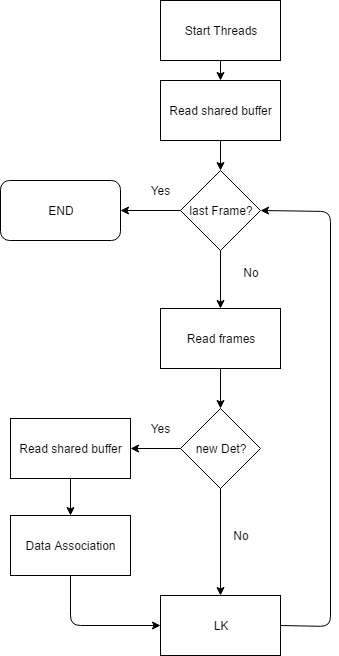
\includegraphics[width=5cm]{flows/arc.png}}
\subfigure[Object detector thread.]{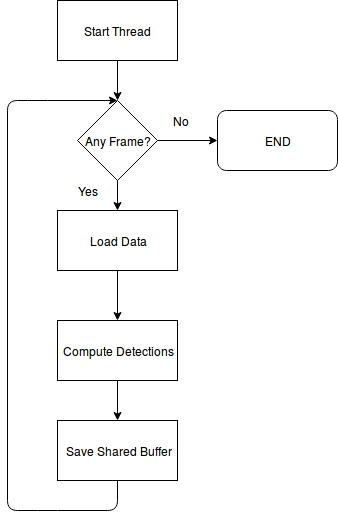
\includegraphics[width=5cm]{flows/detetc.png}}\\


\caption{Flow chart of the system.}
\label{introTracking3}
\end{figure}

We represent each person with a bounding box, in this bounding box we extract some features and compute how they movement through the frames, based on the movement of those features we will infer the movement of the bounding box, therefore, the movement of the person.

\section{System design}

In this section we explain the parts of the algorithm in detail.

\subsection{Object detector by neural networks}



As we stated previously we compute the pedestrian detector based on a CNN. This types of systems are very accurate but slow. We are constraint by its execution time, it takes $0.92$ seconds for compute each detection, this allows us to get a new detection after $30$ frames. 

%\begin{algorithm}
%\caption{Object detection thread}\label{euclid}
%\begin{algorithmic}[1]
%\Procedure{Detection}{}
%%\State $A tracker prodcues a trajectory by tracking the point forward in time$
%%\State $network \gets \textit{patlen}$
%\State $network = network.init()$
%\State $FPS = 30$
%\State $FRAMES SEQUENCES = num of files(sequences)$
%\State $LIST_INDEXs = createList(FPS,FRAMES_SEQUENCES)$
%\For {(each object $LIST_INDEX$)}
%\State $image = read()$
%\State $detection = network.forward(image)$
%\State $sharedVariable = detection$
%\EndFor
%\EndProcedure
%\end{algorithmic}
%\end{algorithm}

We selected the Single shot multibox detector as object detector, in section \ref{valdiation:det} we explain why chose this detector. Finally, in \ref{objectDetector1} we can observe the result of this step.


\begin{figure}[H]
\centering         
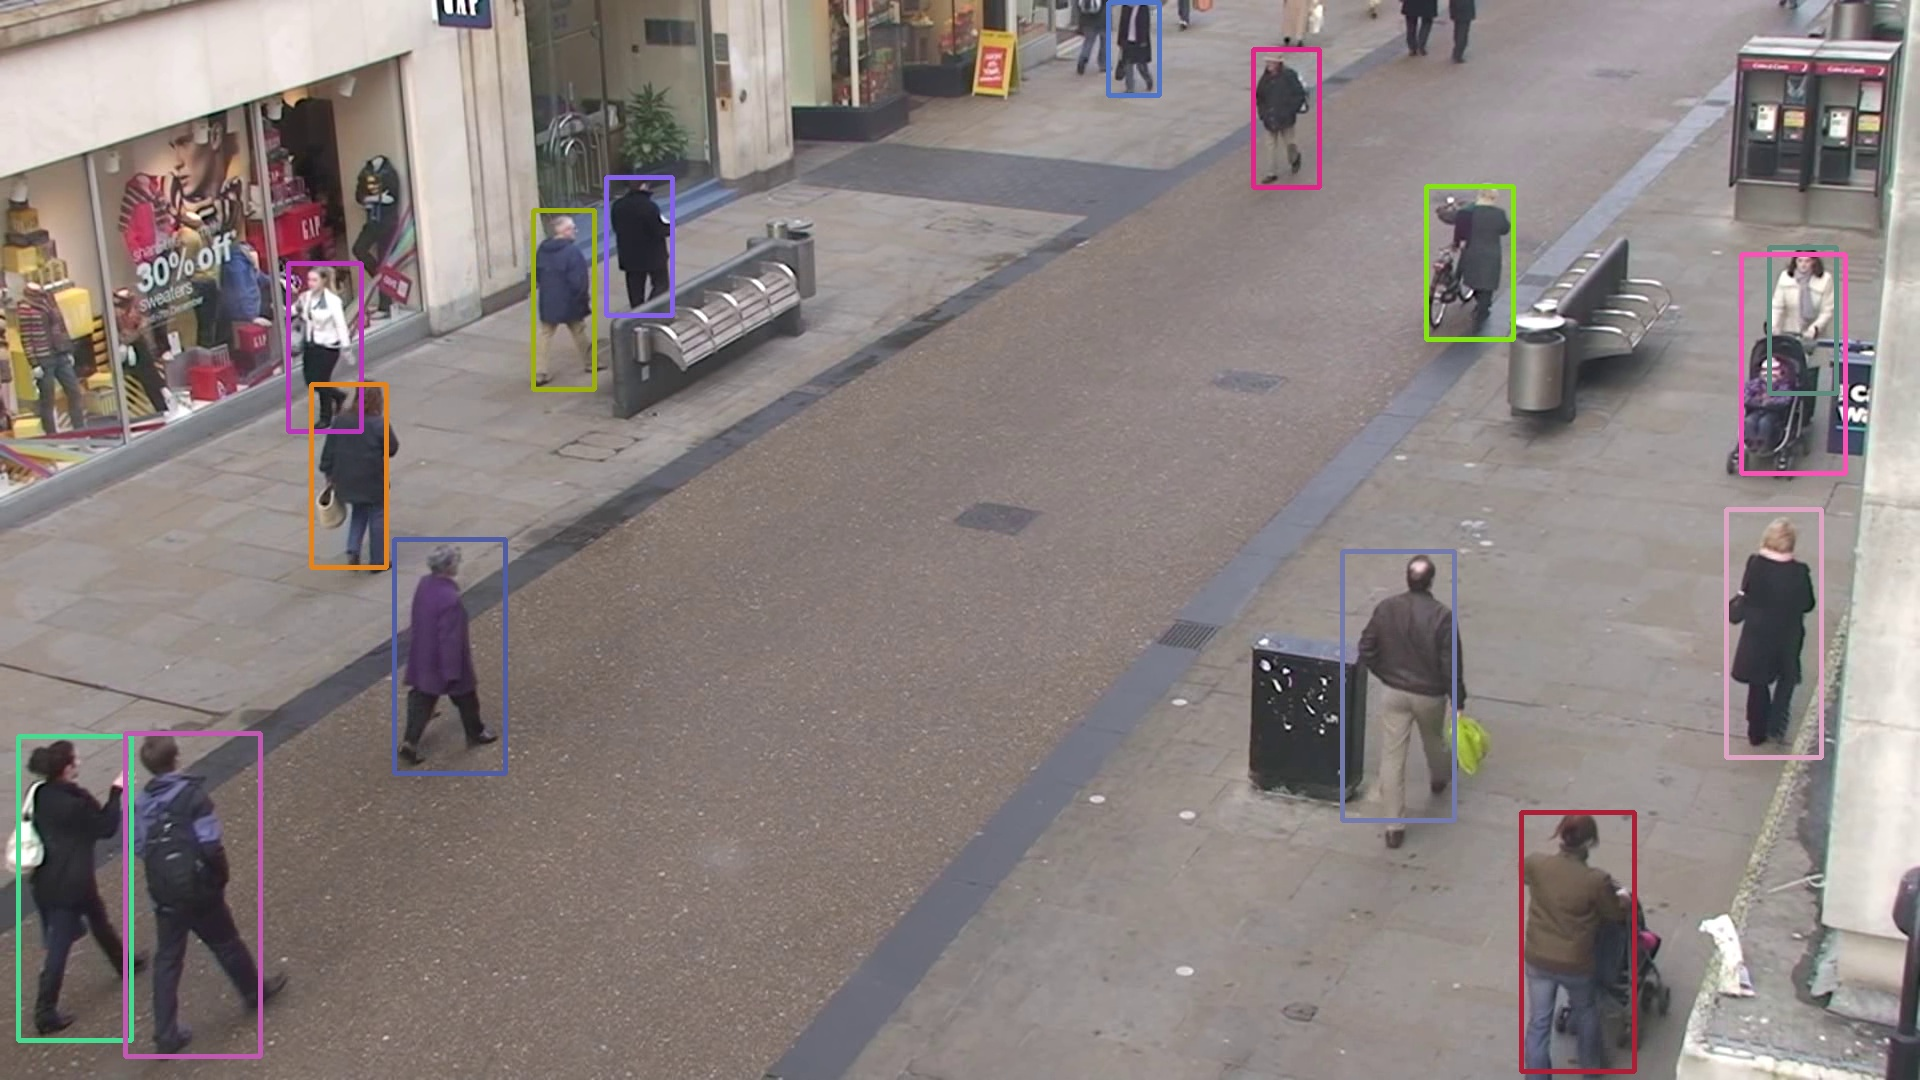
\includegraphics[width=10cm]{intro/deteccions.jpg}
\caption{Detections of the algorithm.} \label{objectDetector1}
\end{figure}


\subsection{Feature tracking}




The essence of the tracking thread it is the tracking module, called LK in the figure \ref{introTracking3}. It stands for Lucas-Kanade algorithm, due it is the method that we used in this work. This module for each detection computes its displacement by computing the displacement of the features inside this bounding box. It computes for each ROI at each step.




%
%\begin{algorithm}
%\caption{Object detection thread}\label{euclid}
%\begin{algorithmic}[1]
%\Procedure{Detection}{}
%%\State $A tracker prodcues a trajectory by tracking the point forward in time$
%%\State $network \gets \textit{patlen}$
%\State $network = network.init()$
%\State $FPS = 30$
%\State $FRAMES SEQUENCES = num of files(sequences)$
%\State $LIST_INDEXs = createList(FPS,FRAMES_SEQUENCES)$
%\For {(each object $LIST_INDEX$)}
%\State $image = read()$
%\State $detection = network.forward(image)$
%\State $sharedVariable = detection$
%\EndFor
%\EndProcedure
%\end{algorithmic}
%\end{algorithm}



For extracting the features, we use the OpenCV routine \texttt{goodFeaturesToTrack()}, this function determines strong corners on an image, according the Shi-Tomasi method. His parameters are the following:
 
\begin{itemize}

\item \texttt{image}, input image

\item \texttt{maxCorners}, maximum number of corners to return. If there are more corners than are found, the strongest of them is returned.
\item \texttt{qualityLevel}, parameter characterizing the minimal accepted quality of image corners.
\item \texttt{minDistance}, minimum possible Euclidean distance between the returned corners.
\item \texttt{mask}, optional region of interest.
\item \texttt{blockSize}, Size of an average block for computing a derivative covariation matrix over each pixel neighborhood.
\item \texttt{useHarrisDetector},  Parameter indicating whether to use a Harris detector.
\item \texttt{k},  Free parameter of the Harris detector.

\end{itemize}

We applied an equalization to the image to obtain more high contrast points, we can observe this in the figure \ref{solution2} and for each ROIs it looks like \ref{solution3}.


\begin{figure}[H]
\centering         
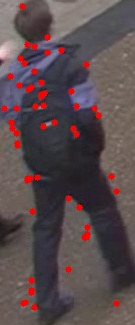
\includegraphics[width=3cm]{implementation/pointsEQU.jpg}
\caption{Shi-Tomasi points on a person.} \label{solution2}
\end{figure}



\begin{figure}[H]
\centering         
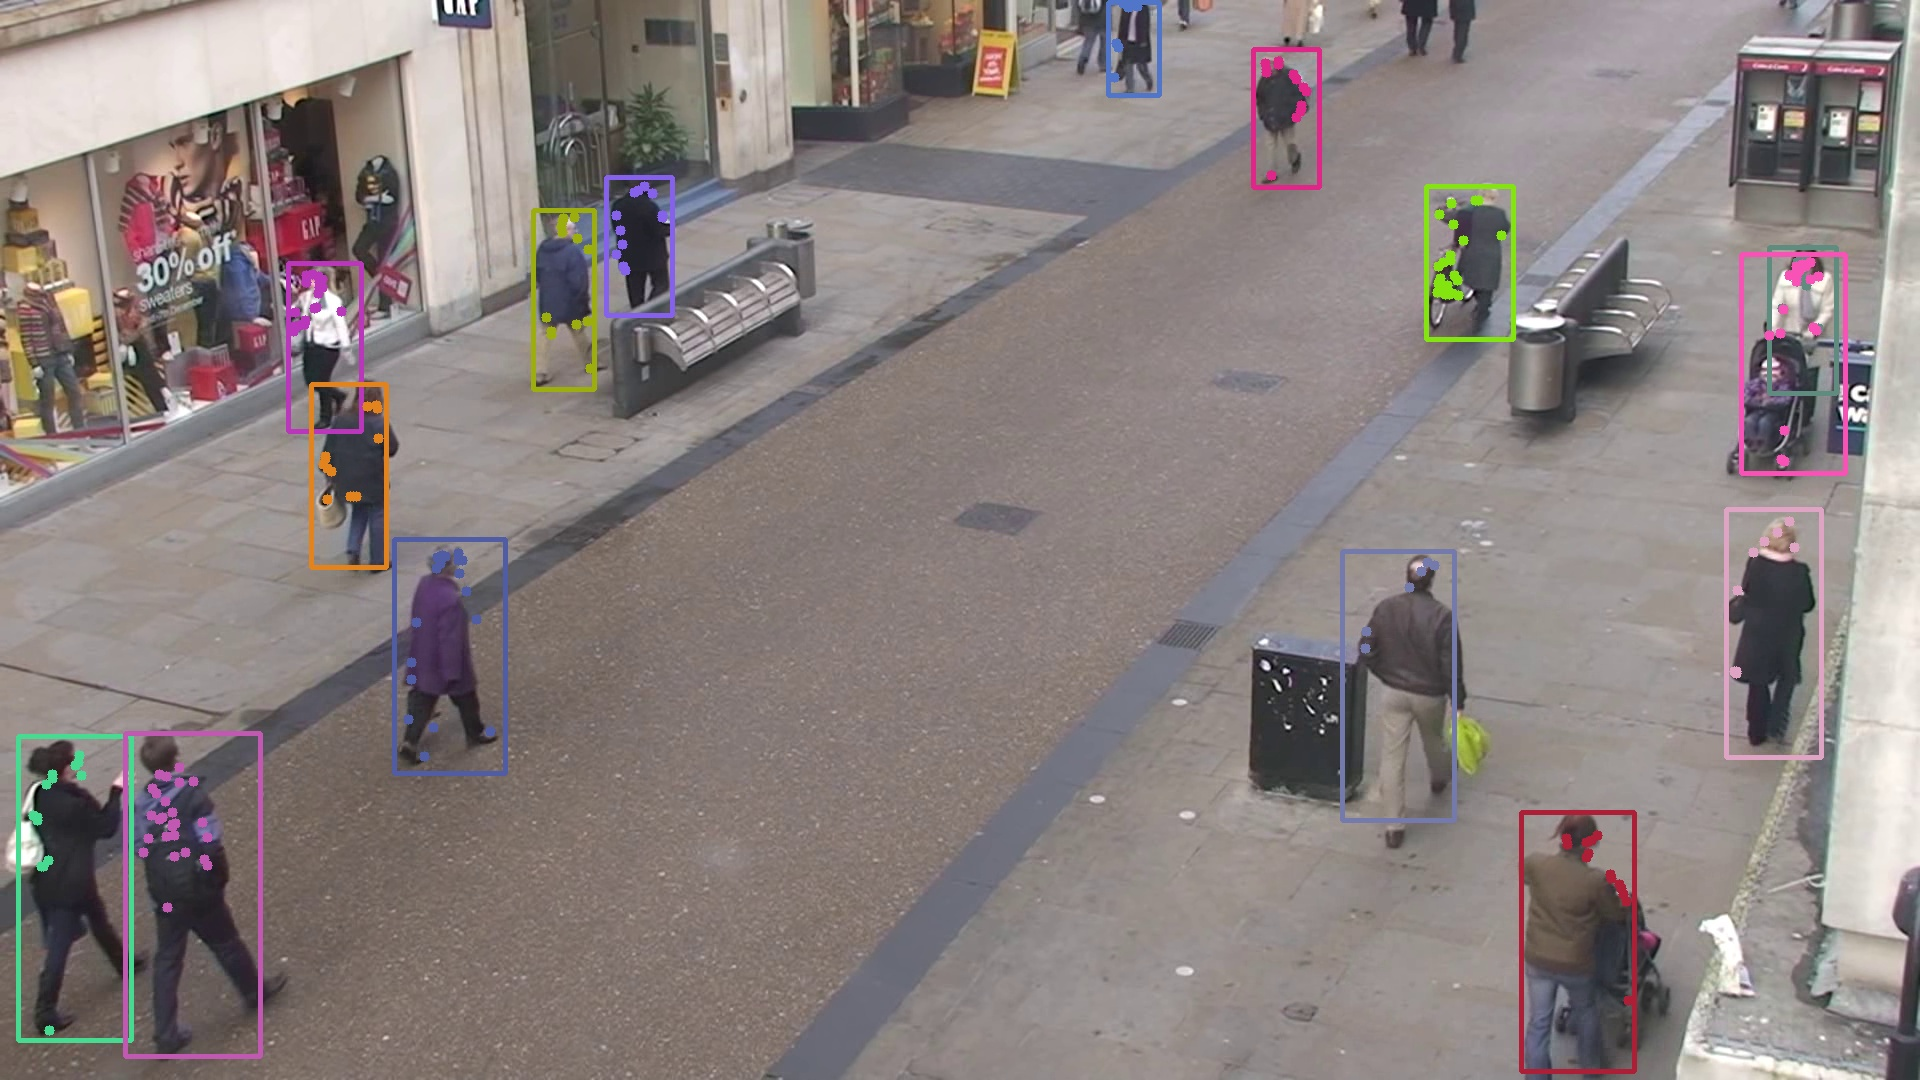
\includegraphics[width=10cm]{intro/pounts.jpg}
\caption{Detections with feature points.} \label{solution3}
\end{figure}

 
%\begin{algorithm}
%\caption{Forward-backward method}\label{euclid}
%\begin{algorithmic}[1]
%\Procedure{FB}{}
%\State $A tracker prodcues a trajectory by tracking the point forward in time$
%\State $i \gets \textit{patlen}$
%%\BState \emph{top}:
%\If {$i > \textit{stringlen}$} \Return false
%\EndIf
%\State $j \gets \textit{patlen}$
%%\BState \emph{loop}:
%\If {$\textit{string}(i) = \textit{path}(j)$}
%\State $j \gets j-1$.
%\State $i \gets i-1$.
%\State \textbf{goto} \emph{loop}.
%\State \textbf{close};
%\EndIf
%\State $i \gets i+\max(\textit{delta}_1(\textit{string}(i)),\textit{delta}_2(j))$.
%\State \textbf{goto} \emph{top}.
%\EndProcedure
%\end{algorithmic}
%\end{algorithm}




Once we have all the detections with their points, we can compute its displacement, to do so,  we used the OpenCV's routine \texttt{calcOpticalFlowPyrLK()}, this function implements a sparse iterative version of the Lucas-Kanade optical flow with pyramids. And his parameters are the following:
 
\begin{itemize}

\item \texttt{prevImg}, first image.
\item \texttt{nextImg}, second image.
\item \texttt{prevPts}, vector of 2D points for which the flow needs to be found. 
\item \texttt{nextPts}, output vector of 2D points containing the calculated new positions of input features in the second image. 
\item \texttt{status}, output status vector, it tells you whether the flow has been found.  
\item \texttt{err}, each element of the vector is set to an error for the corresponding feature.
\item \texttt{winSize}, size of the search window at each pyramid level. 
\item \texttt{maxLevel}, number of pyramid levels.  
\item \texttt{criteria}, parameter, speifying the termination criteria of the iterative search algorithm.
\end{itemize}



For the example's person we can observe the matching between the points of consecuitve frames. Once we have the correspondaces, we compute the displacement as the median of all of them in each dimension. 

\begin{figure}[hptb]
\centering         
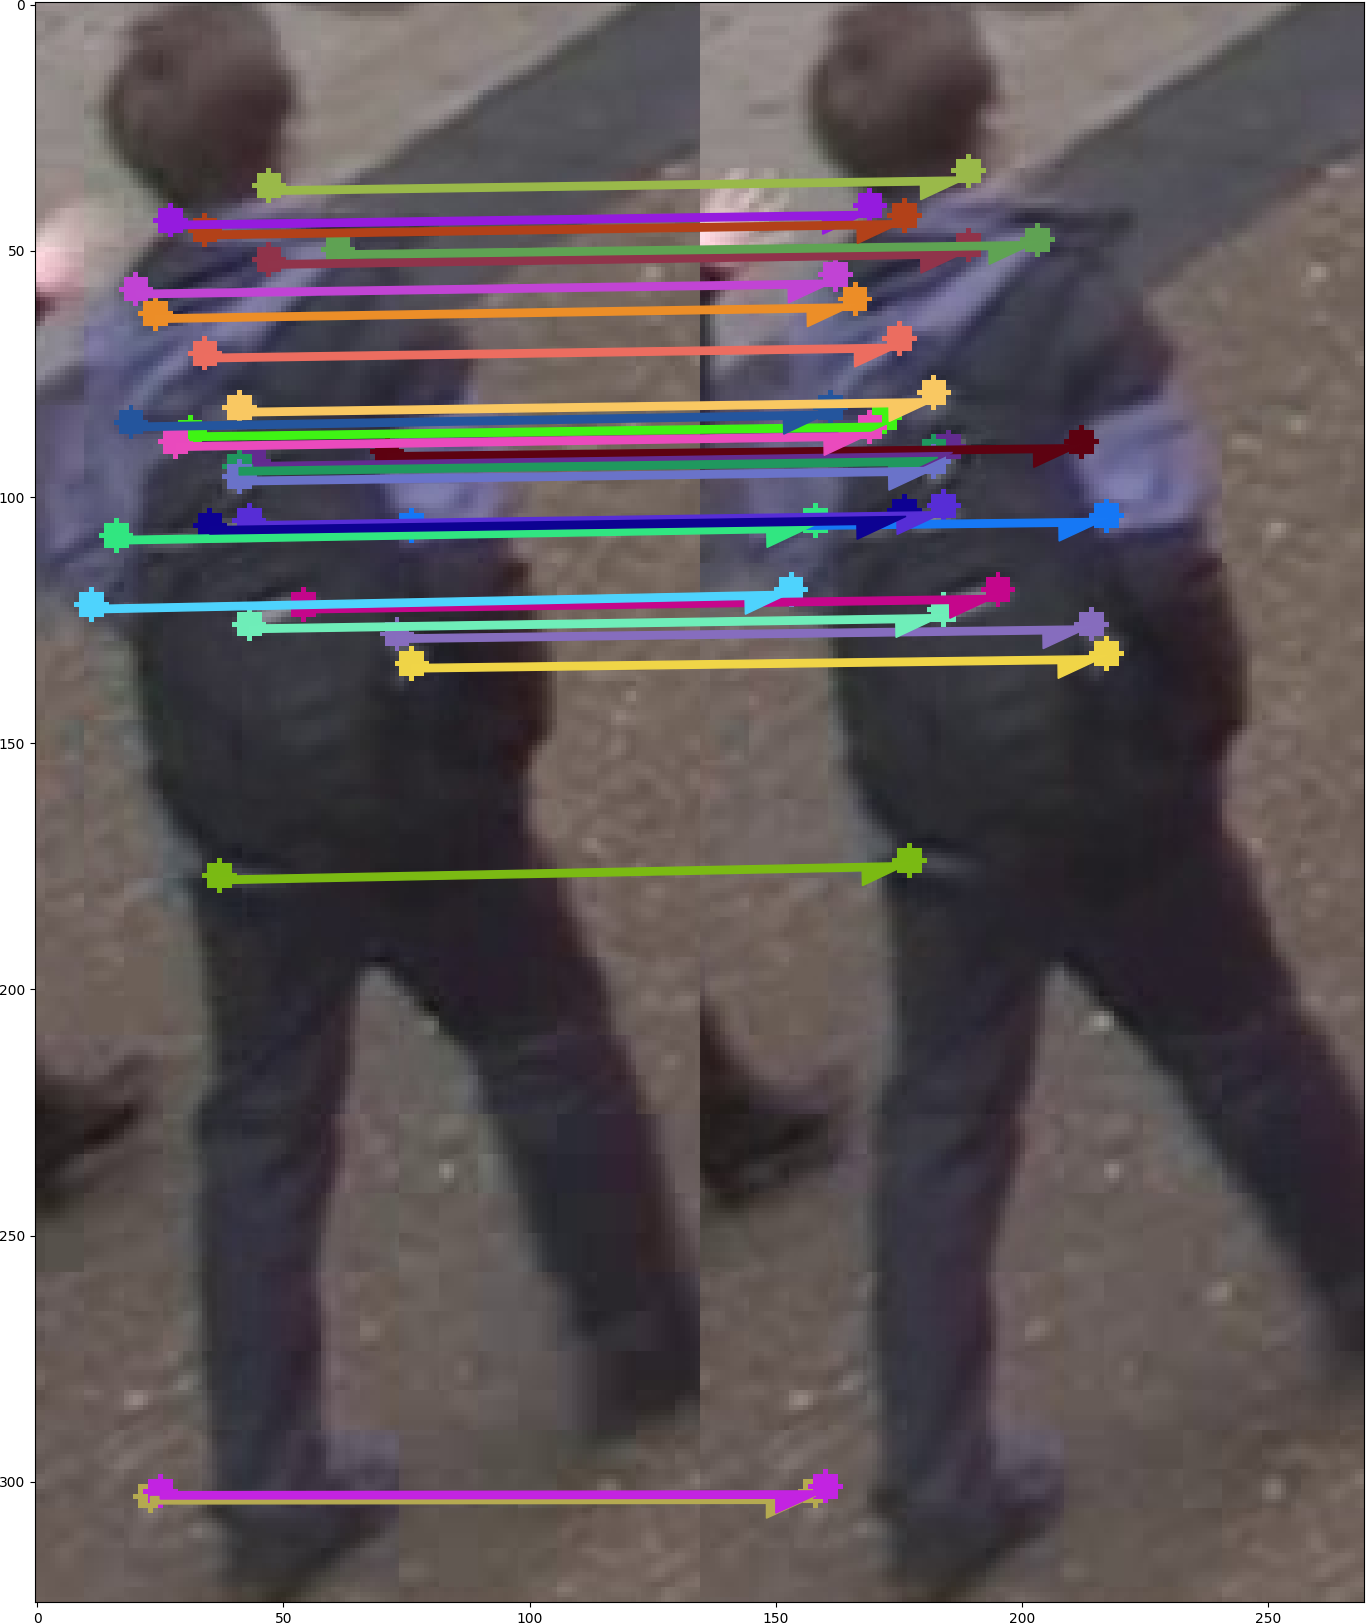
\includegraphics[width=0.3\linewidth]{implementation/matching.png}
\caption{Matched feature points.} \label{solution4}
\end{figure}


In the figure \ref{solution5} we can observe a representation of this dispalcement for each ROI.

\begin{figure}[H]
\centering         
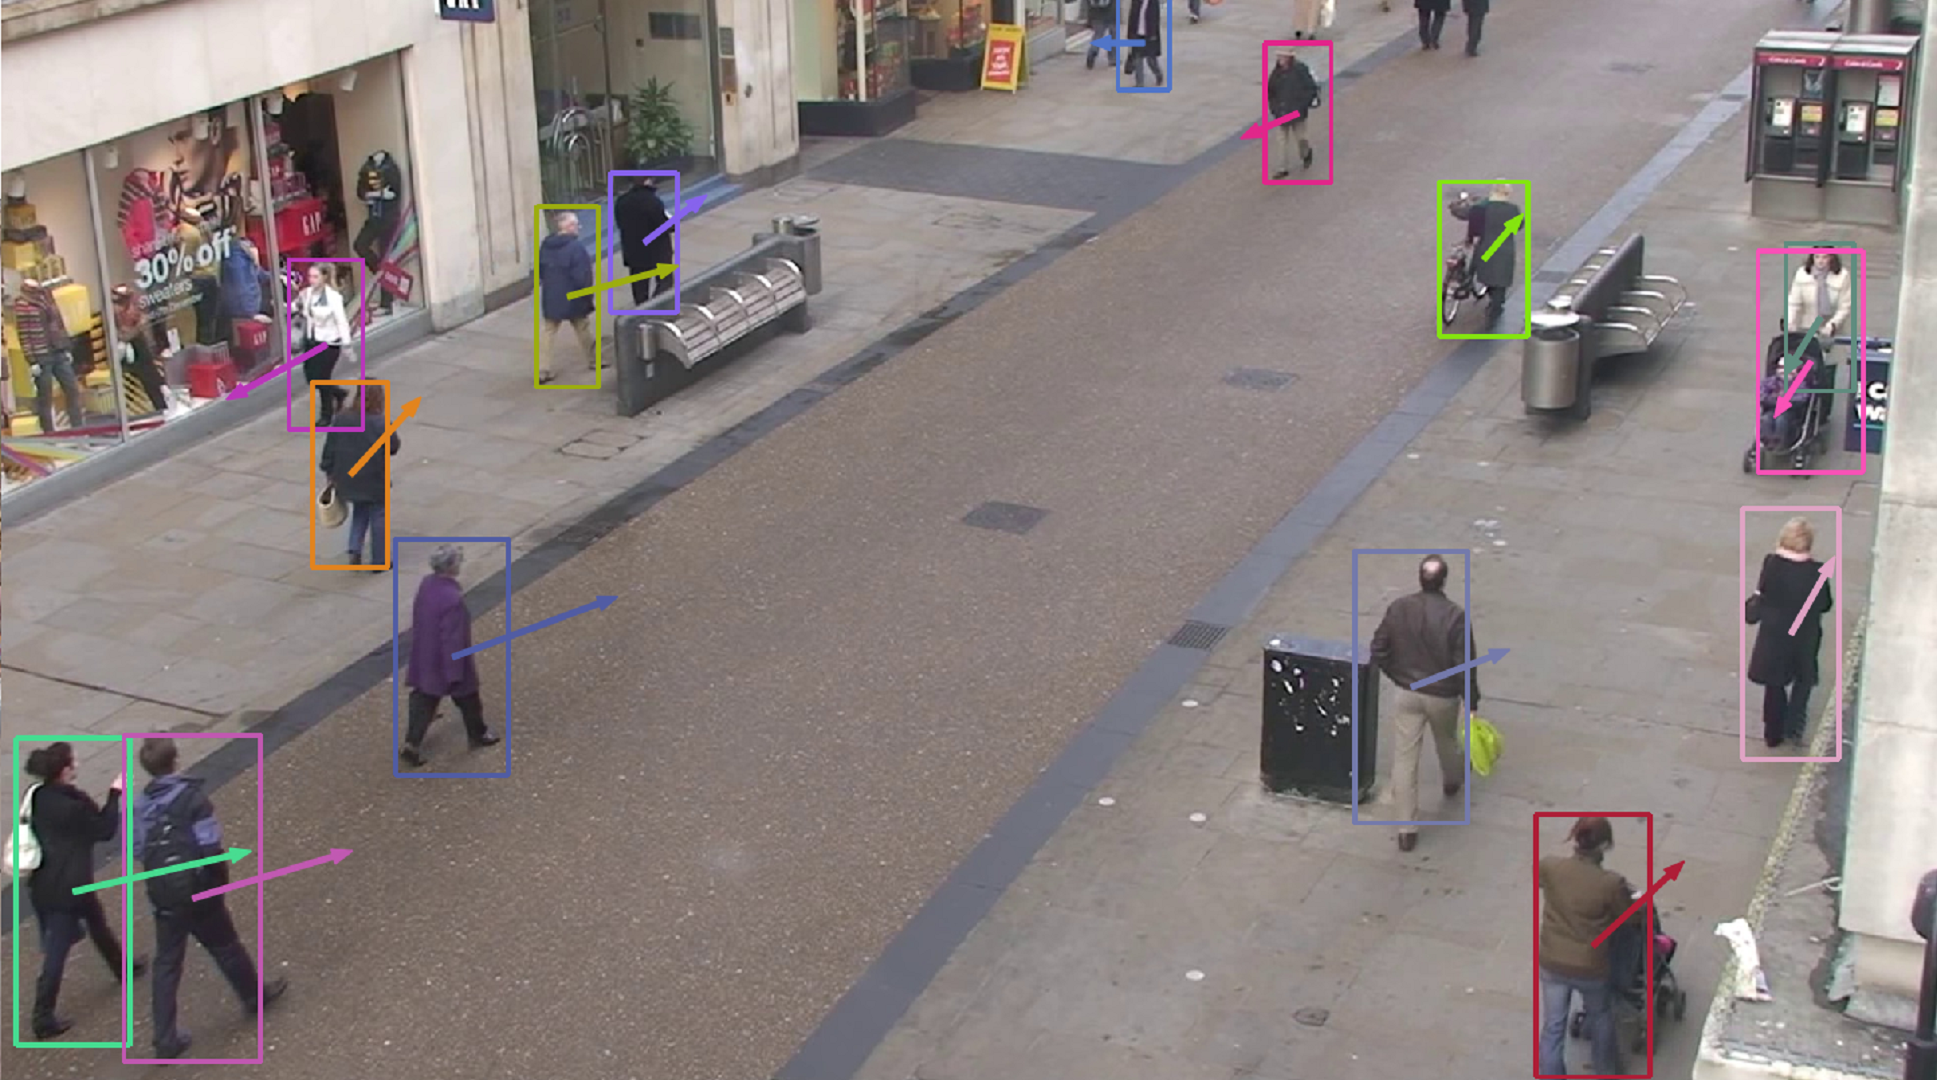
\includegraphics[width=10cm]{intro/alcover2.png}
\caption{Discplacement of each ROI.} \label{solution5}
\end{figure}



Problemas

Next we erased this points, we compute the motion as the median of all the contibutions displacement vectors in each dimension. Also, the scale change is computed as follows: for each pair of points, a ratio between current point distance and previous point distance is computed, bounding box scale change is defined as the median over these ratios. 

At this point, we have an implementation of the tracking algorithm given a set of bounding boxes. Nevertheless, we notice running our algorithm on the dataset, that the bounding box could compute the motion of the assigned pedestrian including the points belonging to another pedestrian who appears also in the bounding box. This interaction will cause a wrong estimation of the movement of the target and eventually the pedestrian will not be embedded by the bounding box. We can observe this event in figure \ref{traccs}.


\begin{figure}[H]
\centering         
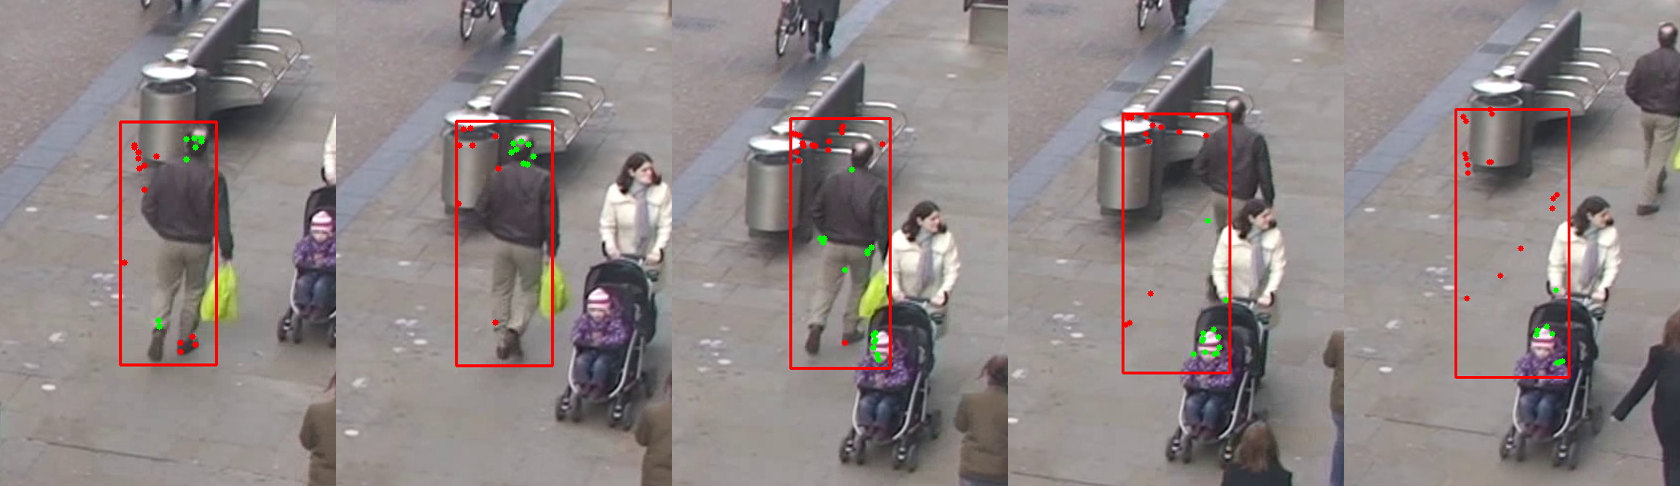
\includegraphics[width=0.9\linewidth]{velocidadas/mateuPont.png}
\caption{Tracking failure.} \label{traccs}
\end{figure}


So, we need a mechanism to detect these failures, therefore we studied how the motion algorithm behaves in these situations. When it has got a trajectory without crossing with other pedestrian, the vertical and horizontal displacement behave like a damping sine wave (if it goes away of the camera)  or amplified sine wave ( if it goes closer to the camera ). But when it has got an interference with another pedestrian, it has an steep change in that wave. We can measure that change as the differences between the current displacement and the previous one normalized by current displacement, if this value overtake a thresolhd, we consider that tracket as a lost tracket. We can observe this process in the next figure \ref{traccs23}, it belongs to previous trajectory \ref{traccs} 


\begin{figure}[H]
\centering         
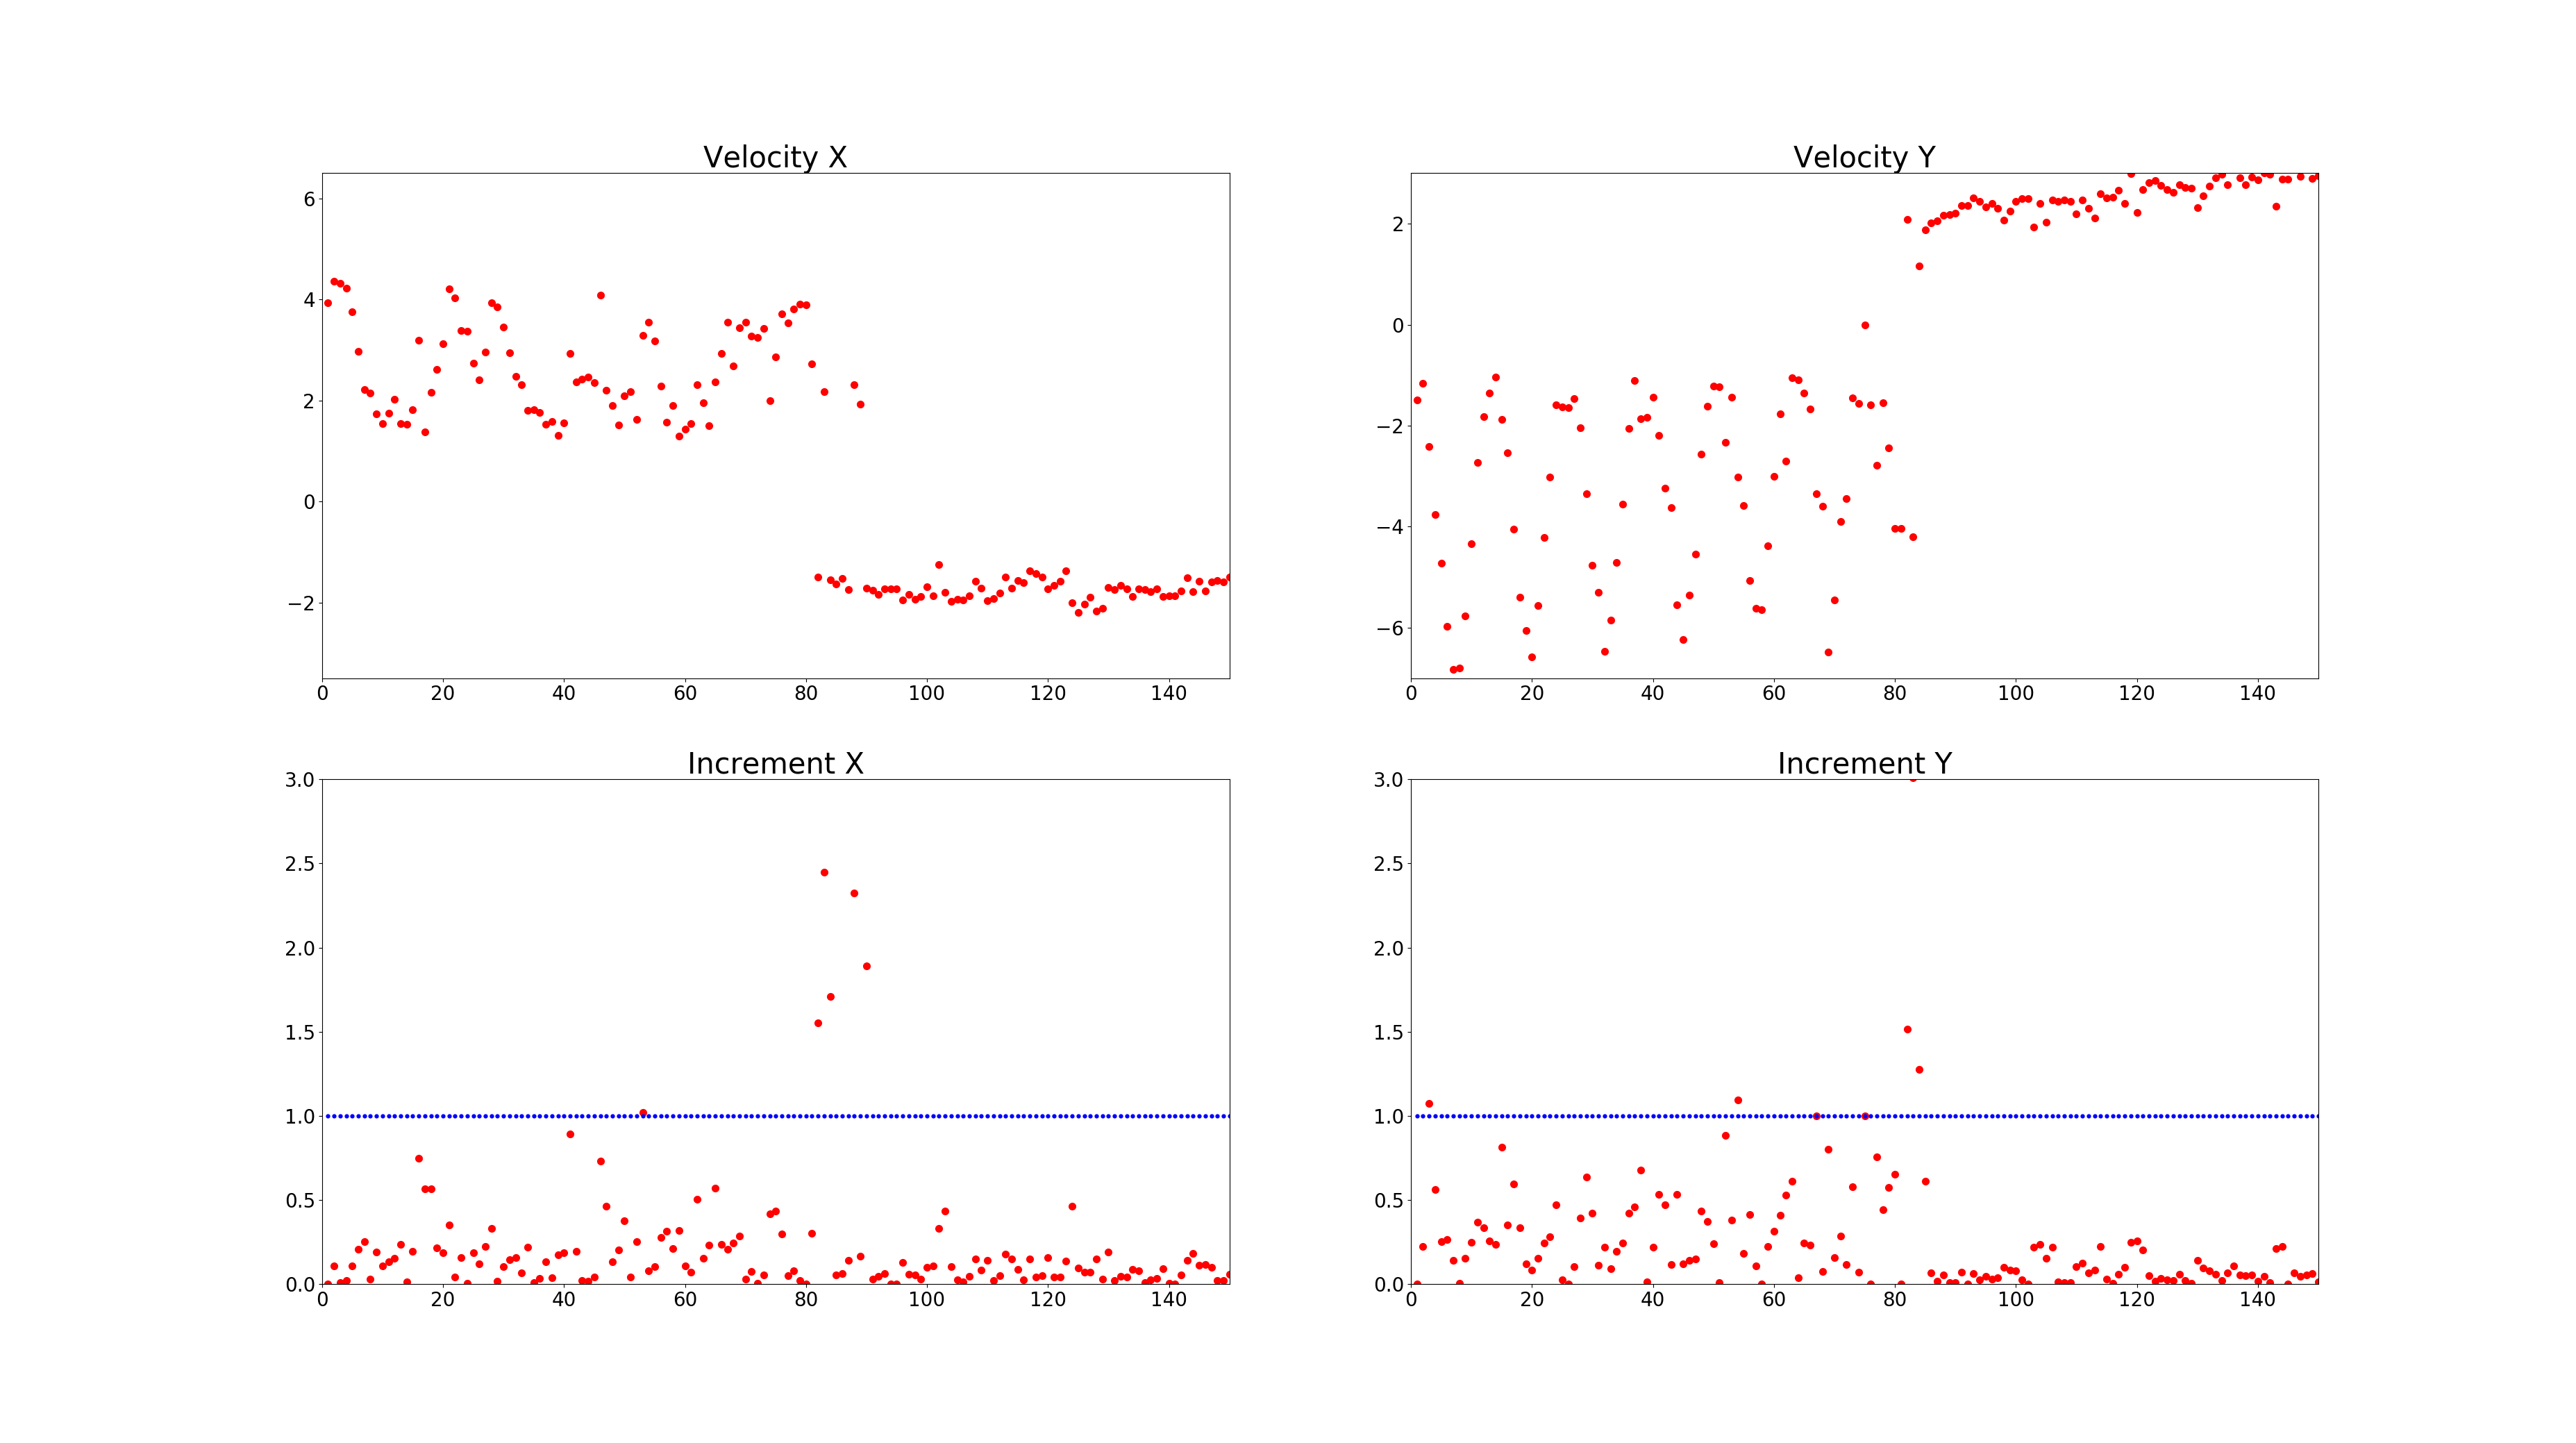
\includegraphics[width=0.9\linewidth]{velocidadas/bad_threshold.png}
\caption{Tracking failure.} \label{traccs23}
\end{figure}


In contrast, when it does not cross with another pedestrian, the displacement does not get disrupt, then the normalized different with the previous displacement gets a low value, we can observe this process in figure \ref{motion2nocoorrect}. We set a threshold to notice this interference and delete this bounding box. We delete them from the current tracking execution, but we save the bounding box for following processings.

\begin{figure}[H]
		
\centering

\subfigure[Trajectory.]{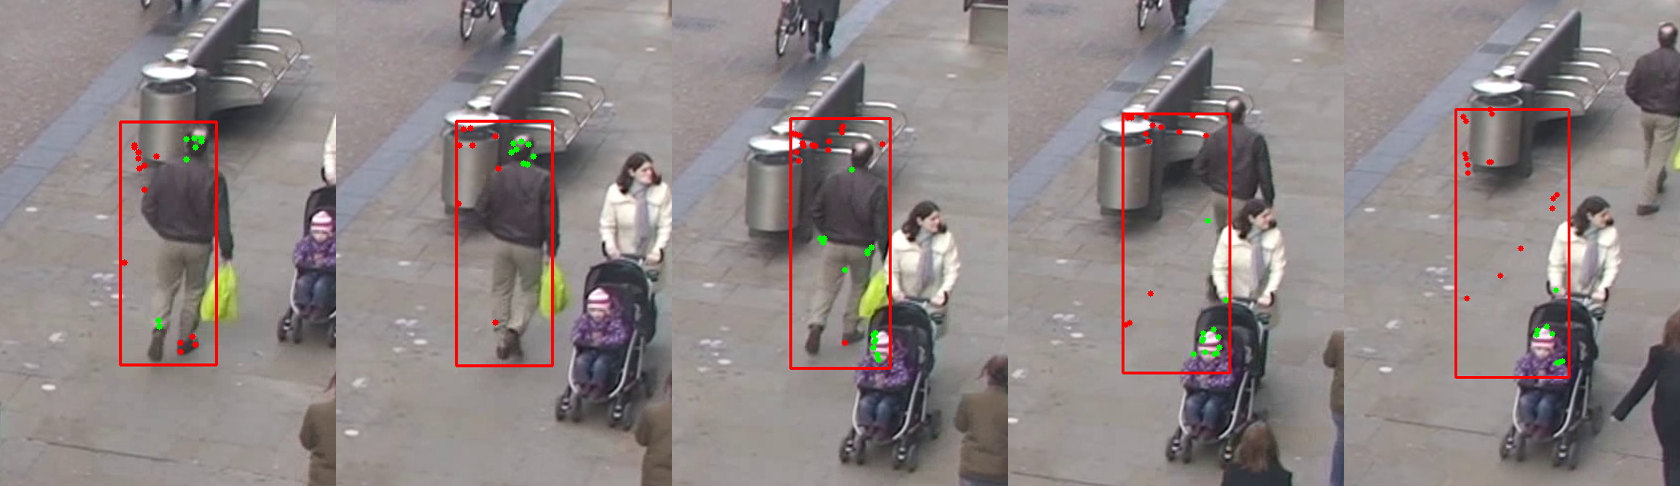
\includegraphics[width=15cm]{velocidadas/mateuPont.png}}\\
\subfigure[Plots movement.]{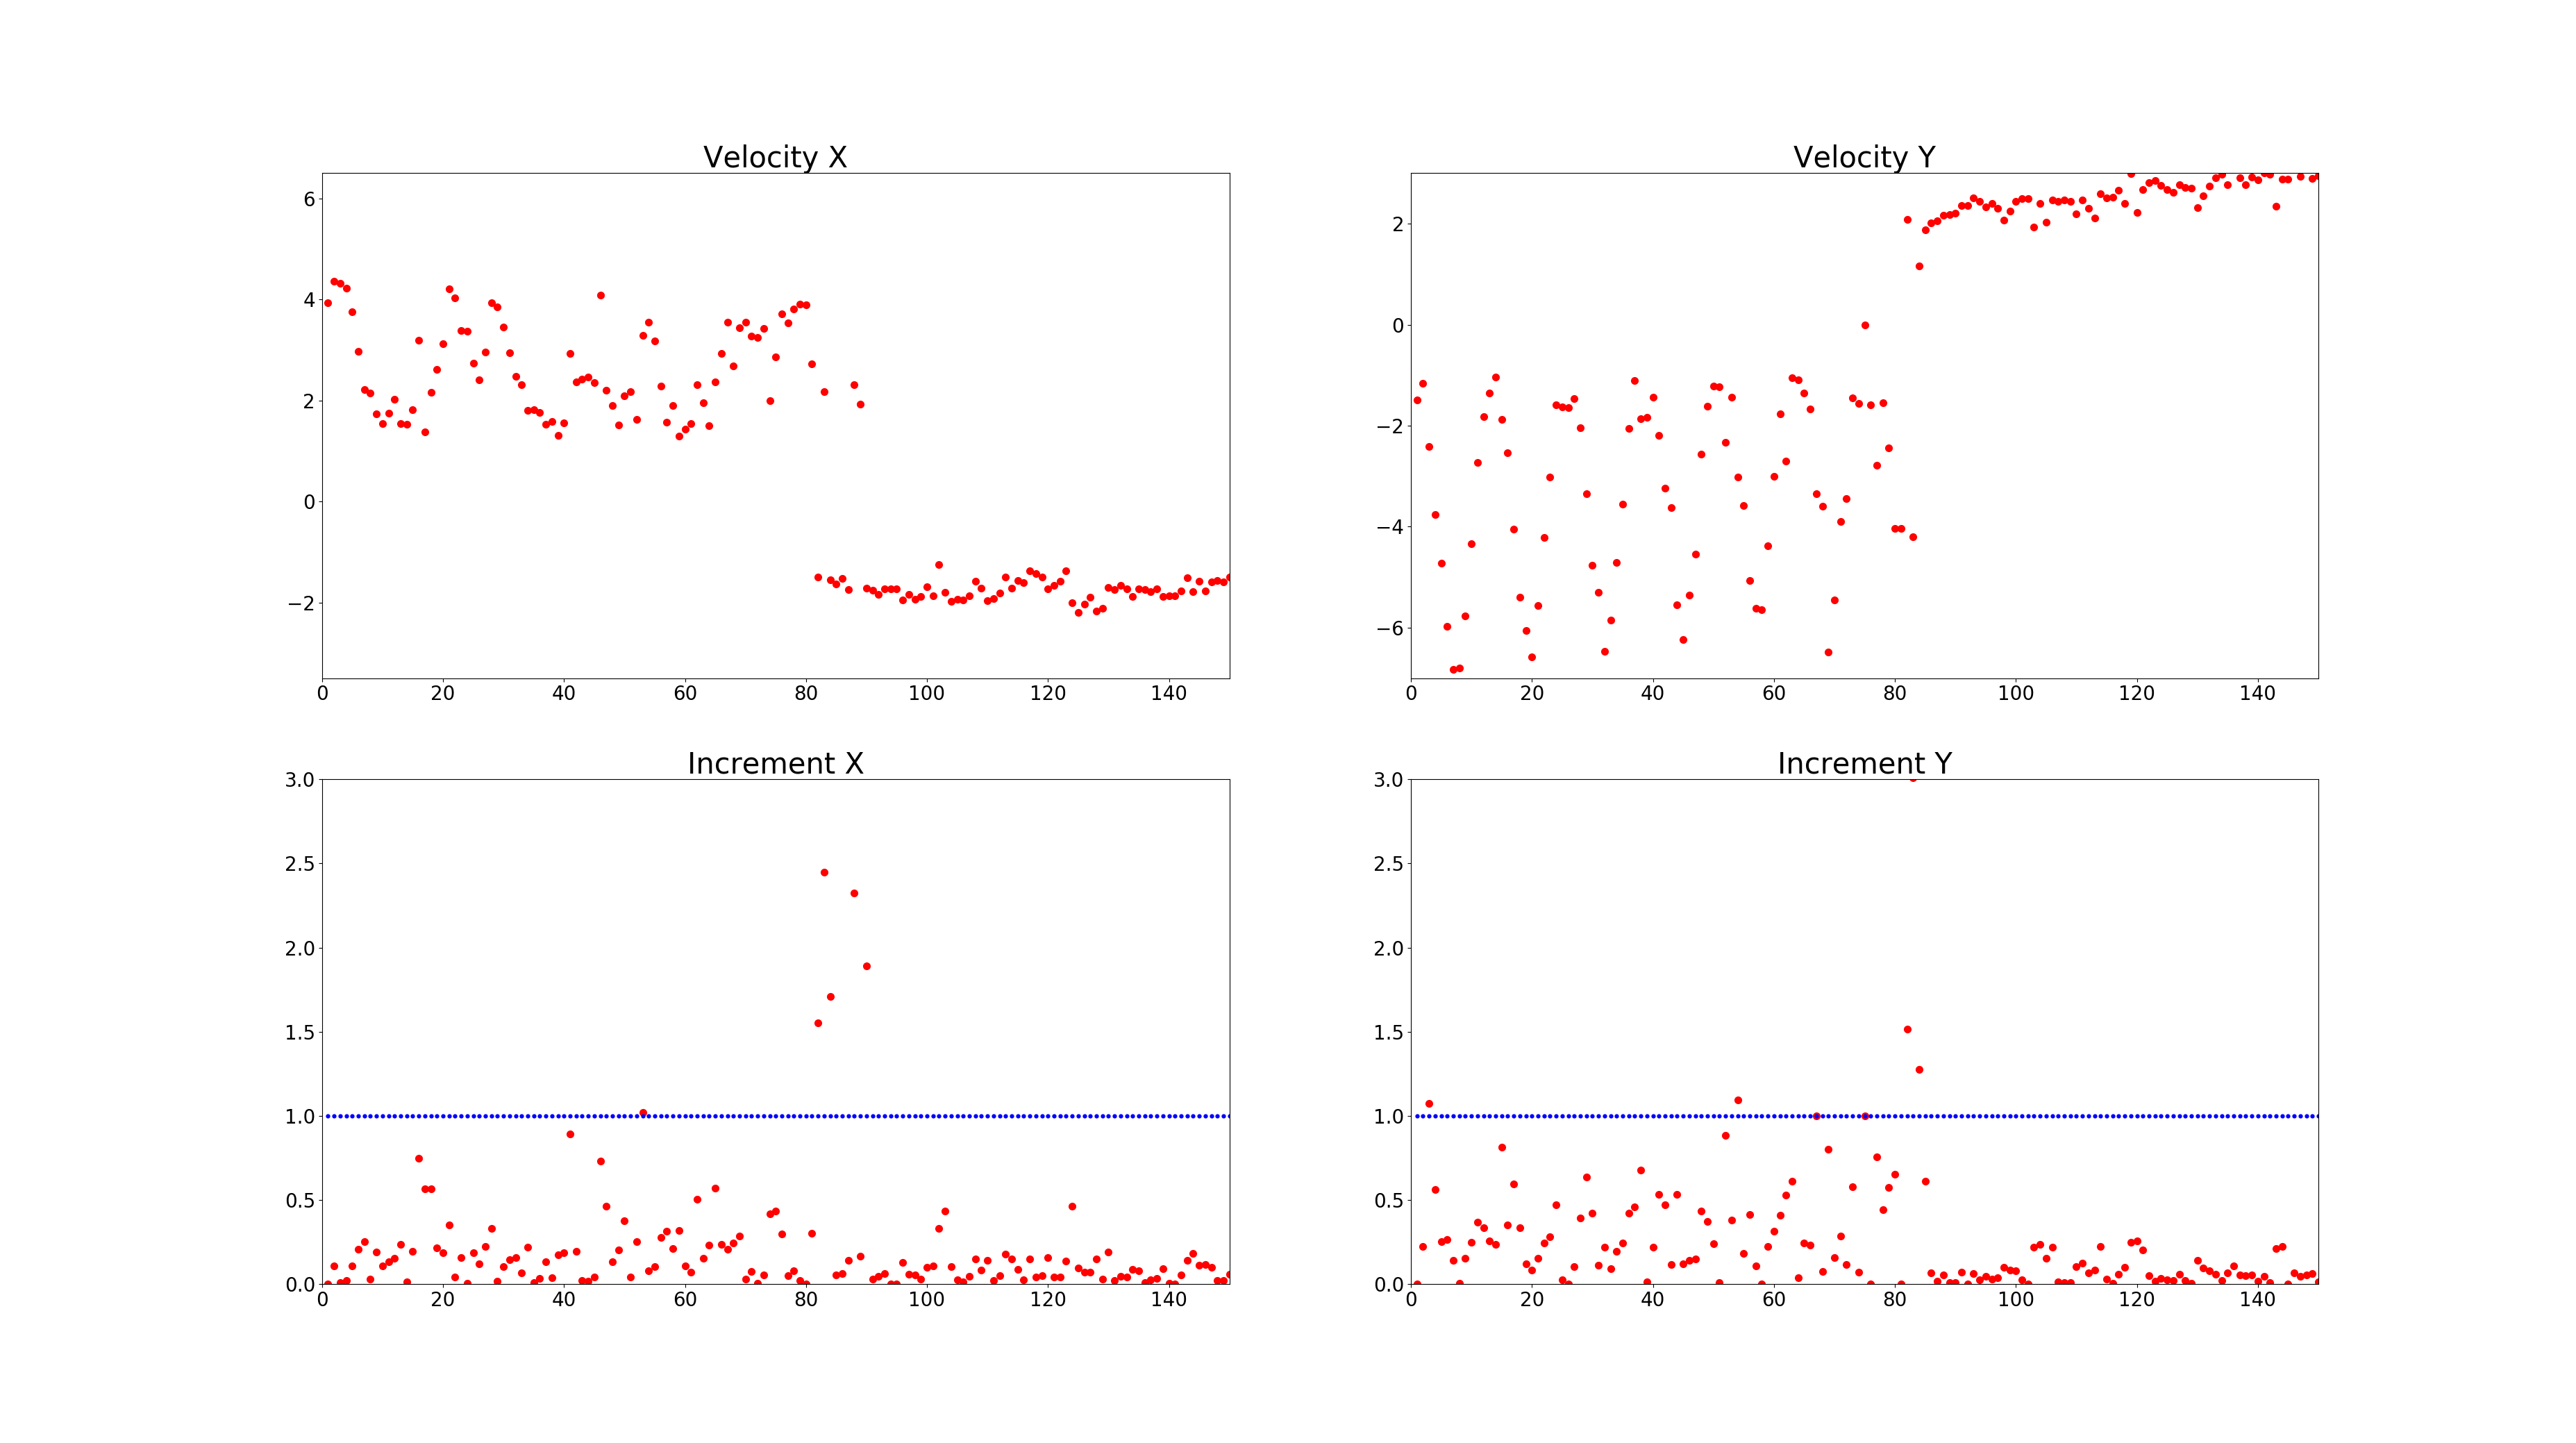
\includegraphics[width=16cm]{velocidadas/bad_threshold.png}}\\
\caption{Wrong trajectory.}
\label{motion2nocoorrect}
\end{figure}













\subsection{Data association}

Once we computed the trajectories, in the next iteration we might have to add a detection, so we need a module to combine these trajectories with detections. Thus, for each pedestrian we distinguish three situations:

\begin{itemize}



\item \textbf{Situation 1}, the tracket has got a nearby detection, then the detection replace the tracket bounding box. This is what is called spatio-temporal constraint.

\item \textbf{Situation 2}, the tracket has not got a nearby detection, then the bounding box tracket continues.

\item \textbf{Situation 3}, the pedestrian has not got a tracket but has got a detection. In this case we need to decided whether this pedestrian is new in the scene or it has been seen before ( it is a lost tracket ).

\end{itemize}

We can observe the procedure for situations number one and two in the figure \ref{data1}, in green colour we can observe the detections and in blue colour the trackets. We defined nearby as the distance between the centres of the boundings boxes, this distance has to be lower than a threshold to be consider nearby. 

\begin{figure}[hptb]
\centering         
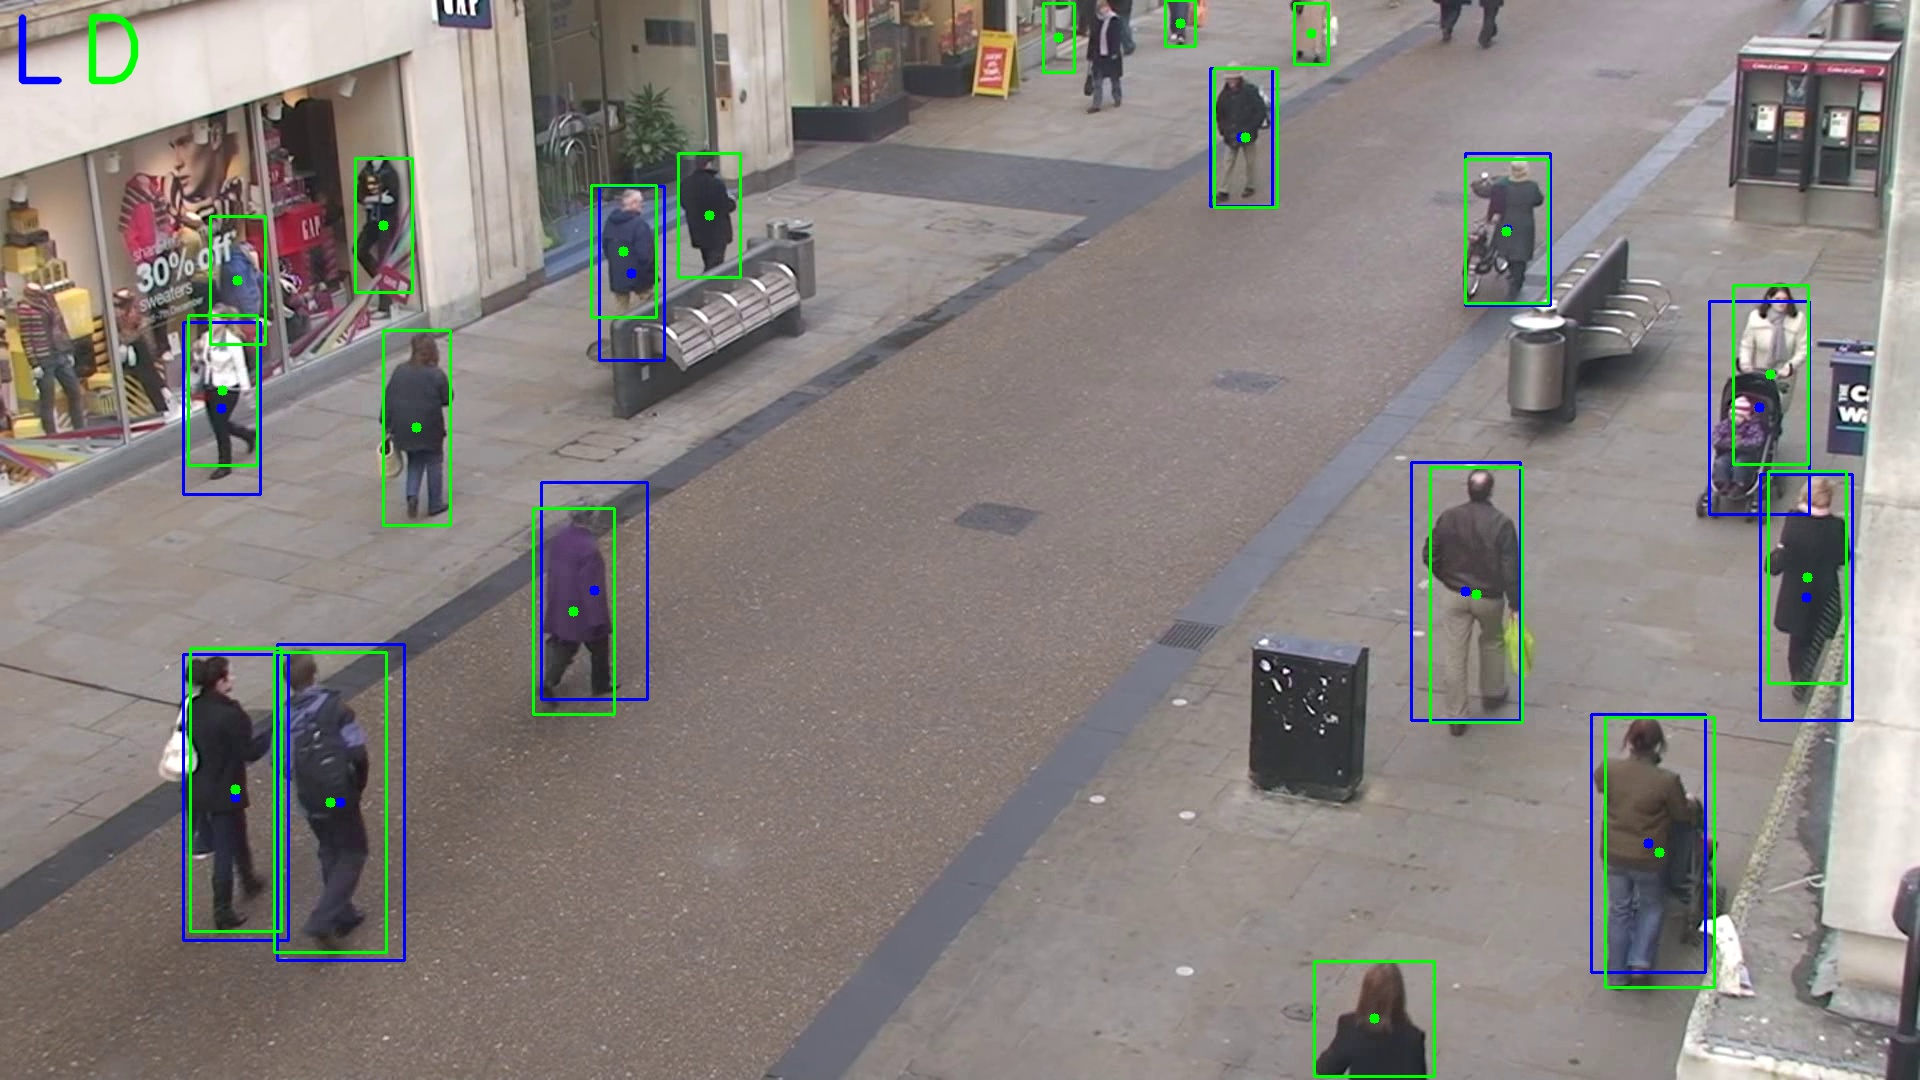
\includegraphics[width=12cm]{lucasKanade/dataAssociation.jpg}
\caption{Spatio-temporal data association.} \label{data1}
\end{figure}


\begin{figure}[hptb]
\centering         
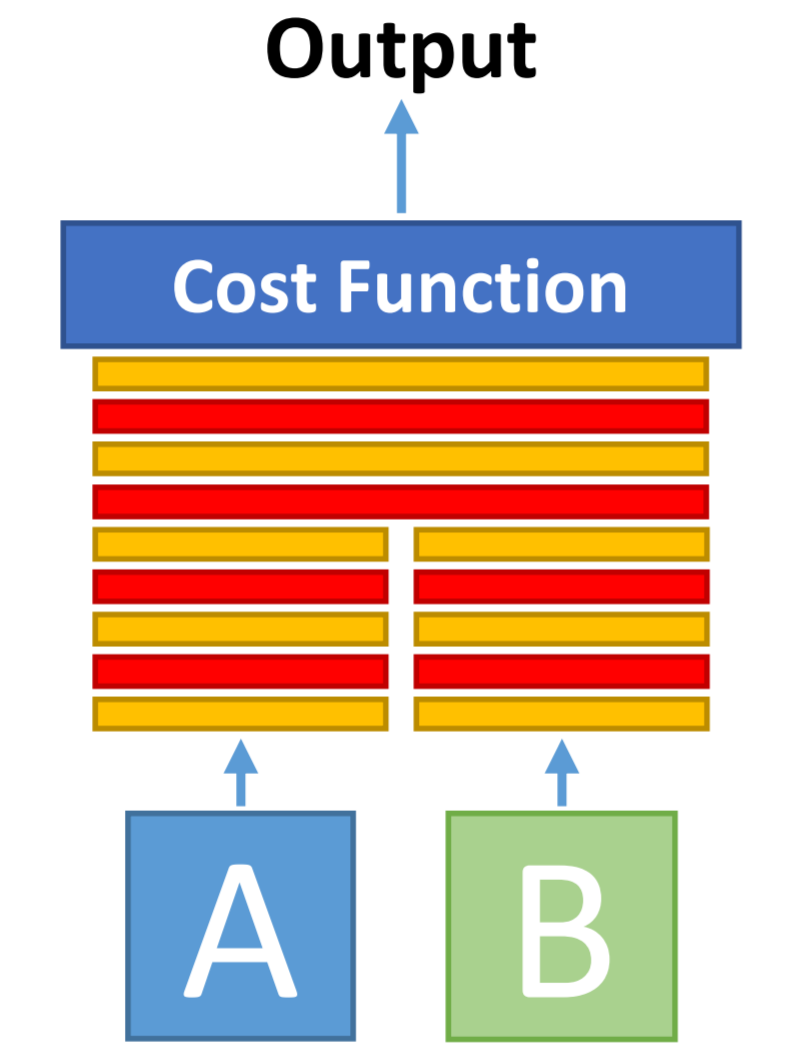
\includegraphics[width=3cm]{siamese/retall2.png}
\caption{Spatio-temporal data association.} \label{data1}
\end{figure}






\lhead[]{CAPÍTULO \thechapter. Datasets and evaluation}
\chapter{Datasets and evaluation procedures}\label{cap.dataset}


In this chapter we explain the datasets and evaluation procedures that we used to adjust our algorithm, or part of it and for experimentally validating the developed solution, allowing an objective comparision between solutions. We explain the three main datasets in this thesis: object detection, tracking, and person reidentification and each of them their measures to evaluate.

\section{Datasets for object detection}

%This section describes the most common datasets used in object detection tasks. Throughout the history of computer vision research datasets have played a critical role.  They not only provide a means to train and evaluate algorithms, they drive research in new and more challenging directions. In order to accomplish this, they provide:


This section describes the most common datasets used in object detection tasks. Throughout the history of computer vision research datasets have played a critical role.  They not only provide a means to train and compare fairly algorithms, they drive research in new and more challenging directions. In order to accomplish this, they provide:


\begin{itemize}

\item a collection of challenging images and high quality annotation.

\item an standard evaluation methodology, so the performance of the algorithms can be compared. 


\end{itemize}



In the next subsections, we will explain several well known international datasets for object detection. These dataset are provided in the context of an international challenges, these challenges look for an improvement on the object detection algorithms. In \ref{instancesCategorydata} we show the comparision of the dataset in two key parameters, number of categories and instances per category, these parameters are critical in the election of one of them.


\begin{figure}[H]
\centering         
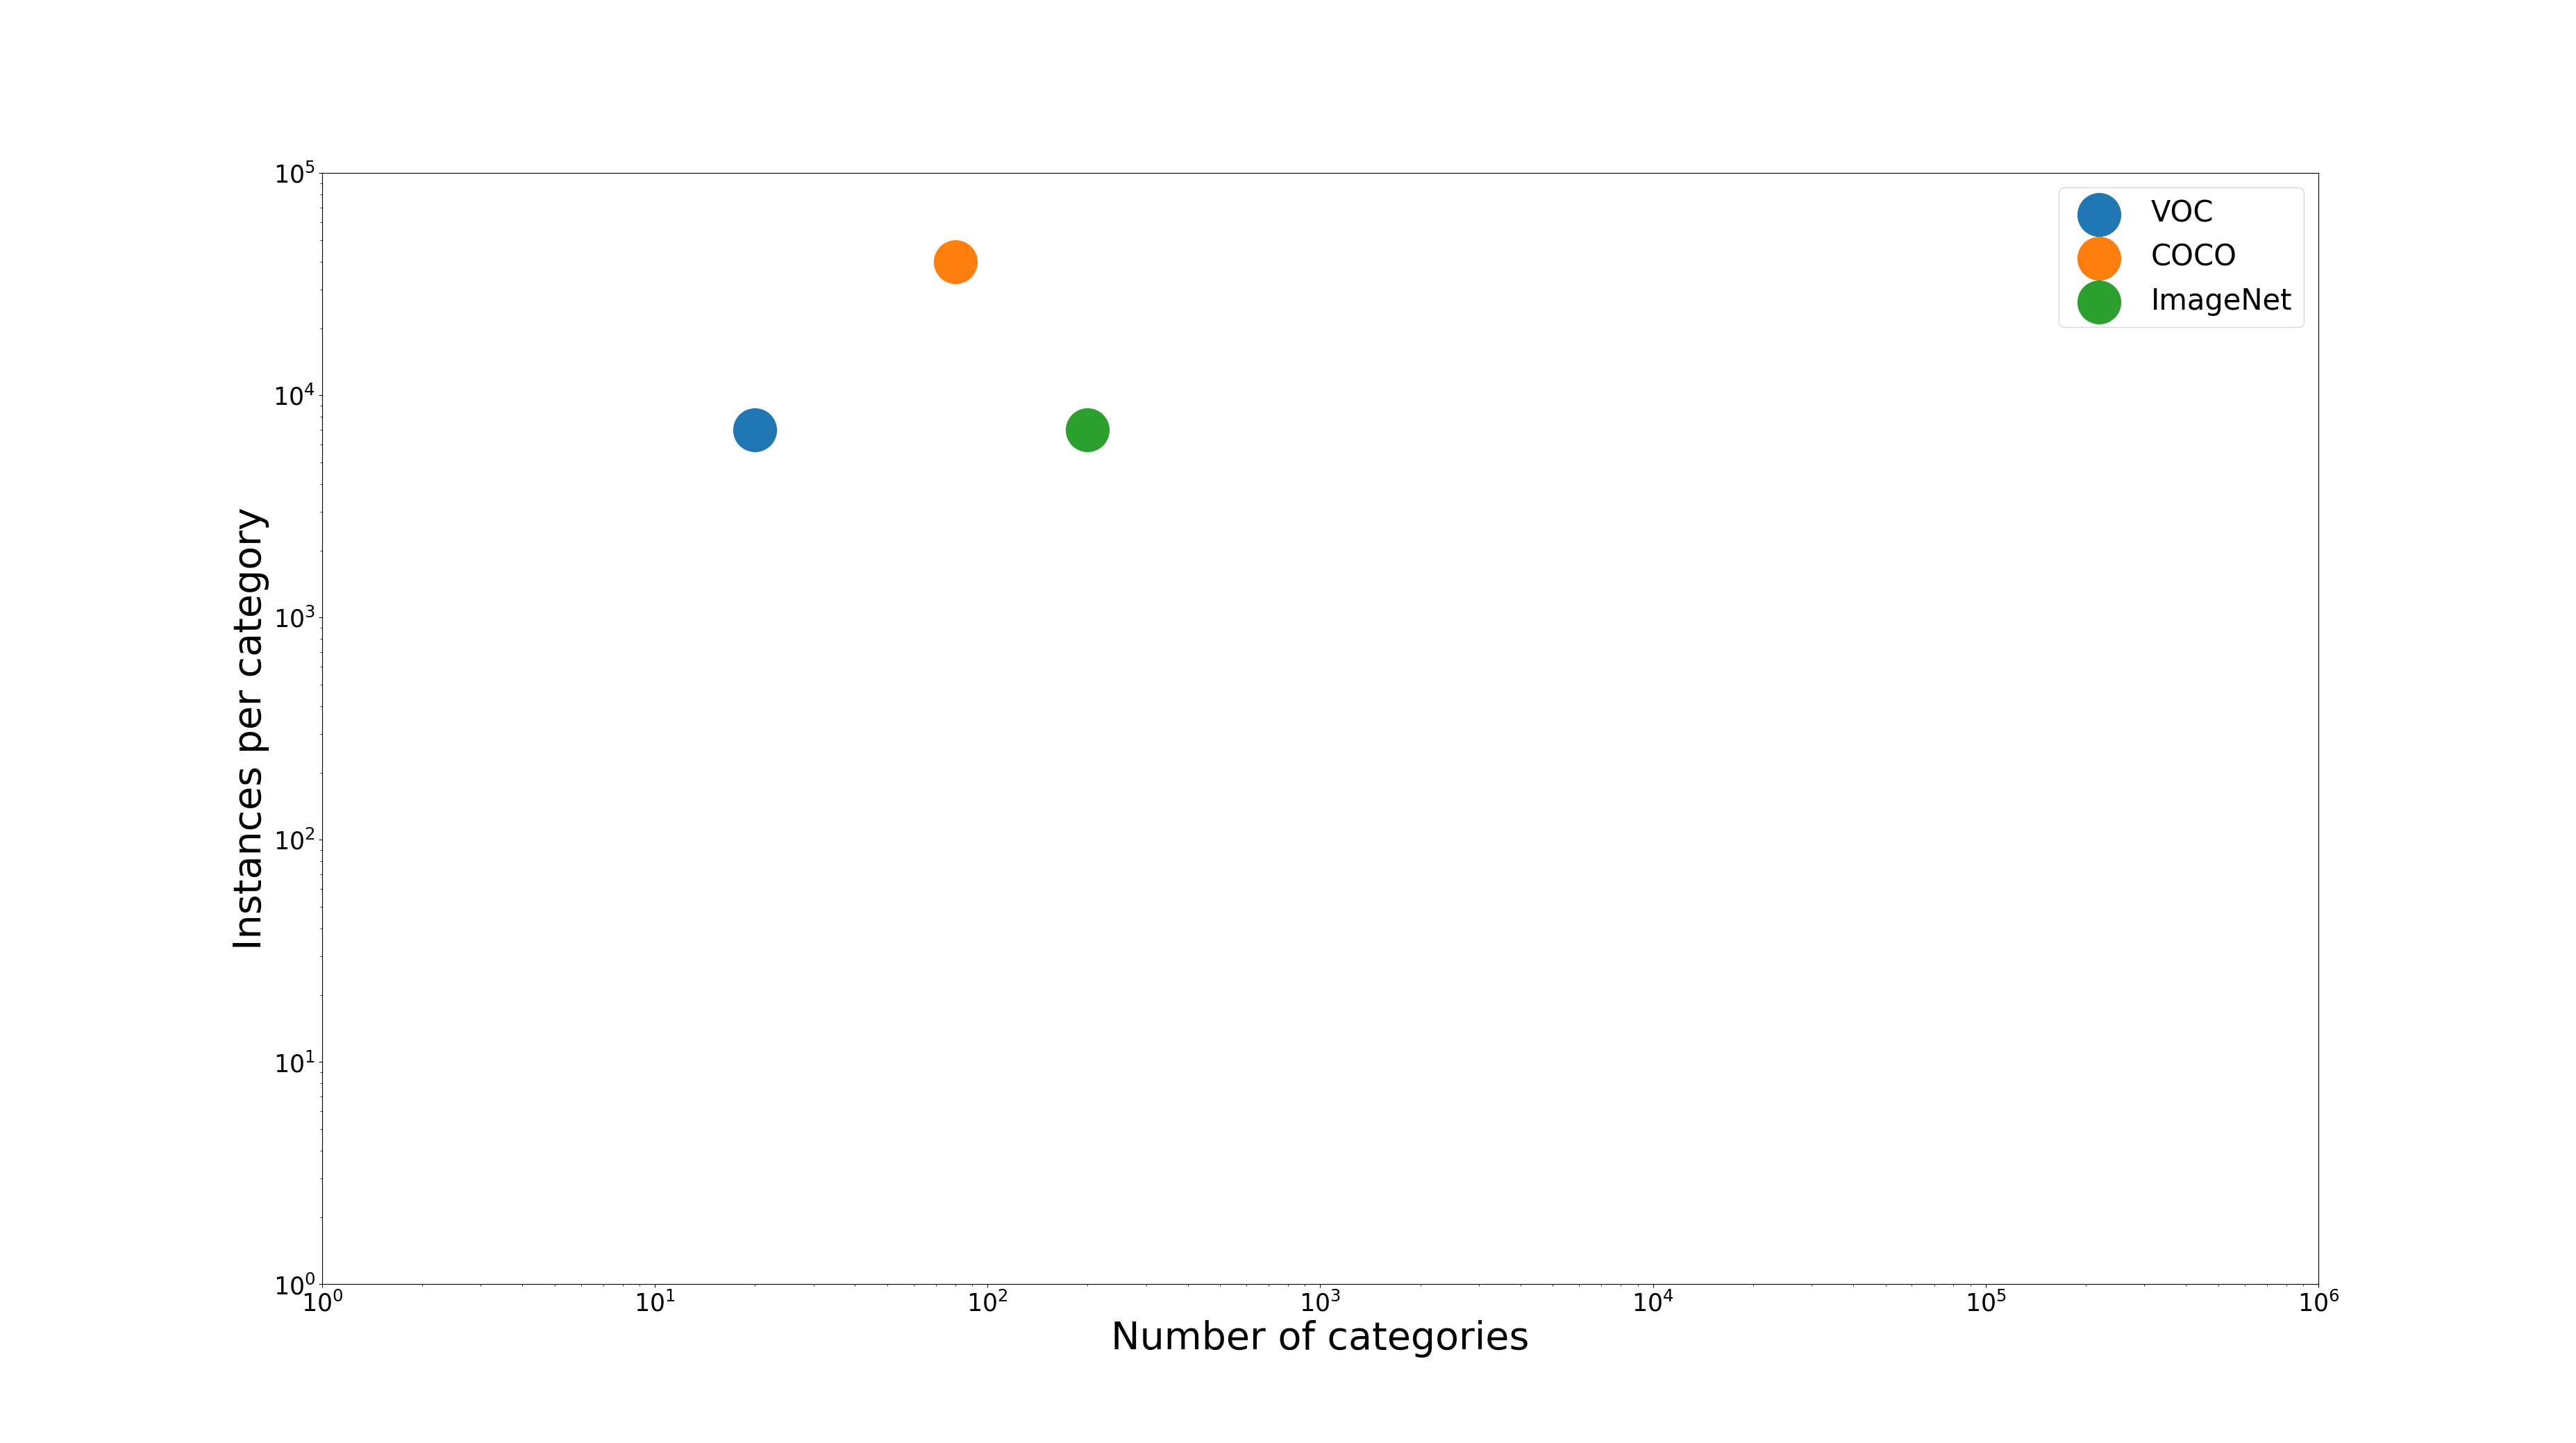
\includegraphics[width=15cm]{datasets/sdad2.png}
\caption{Comparision datasets.} \label{instancesCategorydata}
\end{figure}



\subsection{Pascal Visual Objects Classes}

The Pascal Visual Object Classes (VOC) challenge  \cite{voc07} is a benchmark in visual object category recognition and detection. Organised annually from $2005$ to $2012$, the challenge and its associated dataset has become accepted as one of the landmark benchmarks for object detection. All the images are taken from the \texttt{flickr} consumer photographs website and annotated with the Mechanical turk tool. The most popular editions of the challenge for object detection are those from years $2007$ and $2012$.

The challenge of the year 2007 \cite{voc07website} contains 5000 images in the trainval and test sets, with almost 12000 objects. This was one the first datasets for object detection before the deep learning era. Also, it is very useful for researchers, due it has $2.5$ mean object per image and it is very challenging. In the figure \ref{data07} we can observe the distribution of images and objects instances. 

\begin{figure}[hptb]
\centering         
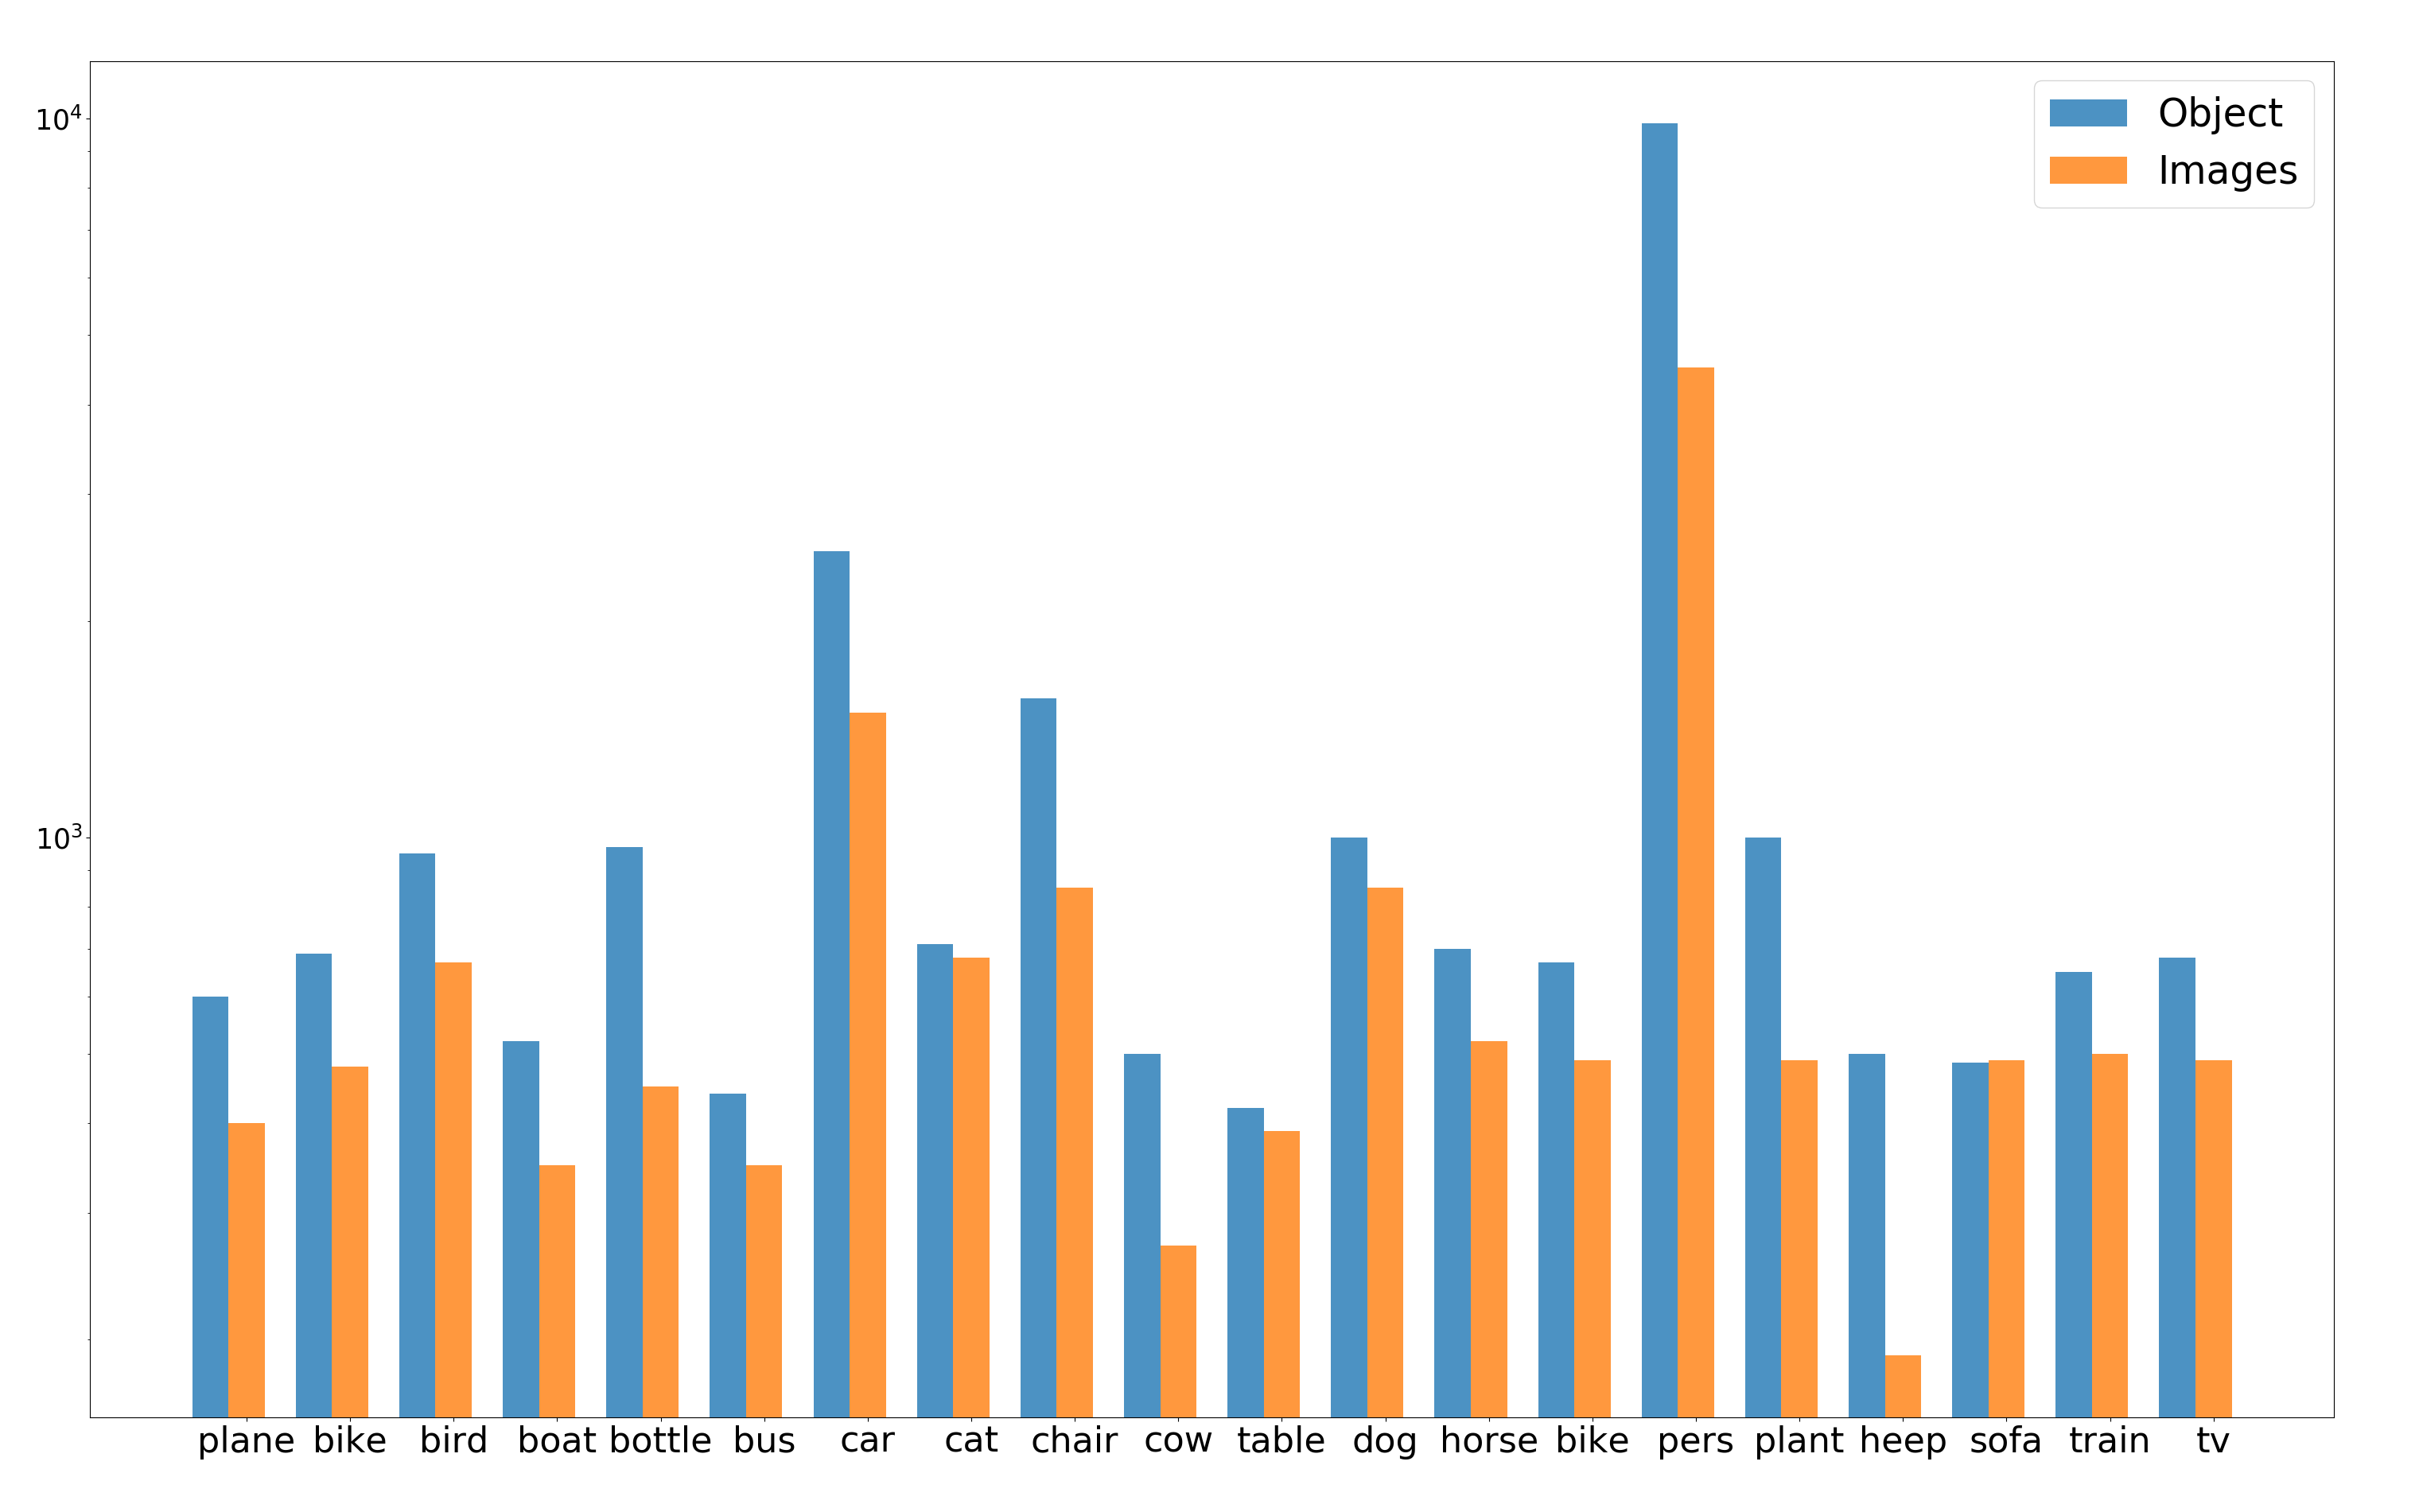
\includegraphics[width=15cm]{datasets/logFinal.png}
\caption{Distribution of VOC07 dataset.} \label{data07}
\end{figure}


In the figure \ref{voc07data} we can observe an example of several images with their ground truth.

\begin{figure}[H]
		
\centering
\subfigure[]{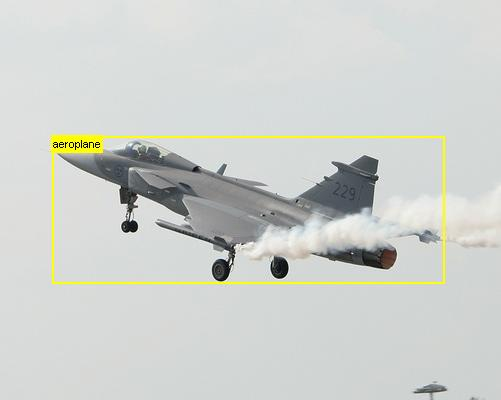
\includegraphics[width=4.9cm]{datasetExample/voc07aeroplane_03.jpg}}
\subfigure[]{\includegraphics[width=5.2cm]{datasetExample/voc07bottle_05.jpg}}
\subfigure[]{\includegraphics[width=5.2cm]{datasetExample/voc07train_05.jpg}}
\caption{Few samples of the VOC07 dataset .} \label{voc07data}

\end{figure}


The 2012's edition \cite{voc12website} is also one of the most used dataset in object detection tasks. It increases the volume of images of the 2007 edition up to 10000 images on trainval and test set and similar quantity of instances per image. In the figure \ref{voc12data} we can observe an example of several images with their ground truth.


\begin{figure}[H]
		
\centering
\subfigure[]{\includegraphics[width=5cm]{datasetExample/voc12bicycle_03.jpg}}
\subfigure[]{\includegraphics[width=5.6cm]{datasetExample/voc12bird_01.jpg}}
\subfigure[]{\includegraphics[width=5cm]{datasetExample/voc12dog_01.jpg}}
\caption{Few samples of the VOC12 dataset .} \label{voc12data}

\end{figure}


The datasets from Pascal challenge are very useful to test object detection algorithms, their quantity is very handy ( a few thousands of images ) and contains a challenging quantity of objects per image, very interesting for the algorithms. But its little amount of images does not permit to train a network on this dataset, although it can be used to finetune the network.


\subsection{ImageNet}



ImageNet project \cite{imagenet} with the challenge ImageNet Large Scale Visual Recognition Challenge [ILSVRC] was the first large-scale database, temporally developed to supply the deep learning techniques, eager of feed with tons of images. ImageNet aims to populate the majority of the 80000 synsets of WordNet with an average of 500-1000 clean and full resolution images. The collection was based on the query of that words on several image search engines and human refined on the Amazon Mechanical Turk platform. It can be downloaded from here \cite{imagenetWebsite}.

In 2016, the project collects more than 10 million of annotated images with 1000 classes. Although its main purpose is image classification, it has an object detection challenge with $200$ categories with over a 1 million images with annotated objects. In the figure \ref{imagenetdata22} we can observe an example of several images.

\begin{figure}[H]
		
\centering
\subfigure[]{\includegraphics[width=5.2cm]{datasetExample/imageNet0.jpeg}}
\subfigure[]{\includegraphics[width=3.95cm]{datasetExample/imageNet1.jpeg}}
\subfigure[]{\includegraphics[width=5cm]{datasetExample/imageNet2.jpeg}}
\caption{Few samples of the ImageNet dataset .} \label{imagenetdata22}

\end{figure}

The datasets for the ImageNet challenge are not used to much in object detection tasks, it contains a few instances per image. This did not encourage researcher to use it. Although it is used to train 
neural networks in image classification tasks. Although those trained architectures can be incorporated in the object detection algorithms.


\subsection{COCO}

The Microsoft Common Objects in Context also known as COCO dataset \cite{coco}, is a dataset that addresses the three core research problems in scene understanding:


\begin{itemize}

\item detecting non-iconic views of objects. For many datasets most of the objects have an iconic representation, they appear unobstructed, near the center of the photo and with their canonical shape. So in this dataset, they included images to struggle the object recognition task, like objects in the background, partially occluded, amid clutter. Therefore, reflecting the composition of actual everyday scenes.

\item contextual reasoning between objects. Nowadays natural images contain multiple objects, and their identity can only be solved using context, due to small size or ambiguos appearance in the image, so in this dataset, images contain scenes rather isolated objects. 

\item the precise 2D localization of objects, also the detailed spatial understanding of object layout will be a core component of an image understanding system, so this dataset struggle to do so.



\end{itemize}


So, the three main tasks of this challenge are object classification, object detection and semantic scene labelling. This dataset contains 91 object categories, with 2.5 million labelled object instances in 328 thousand images, labeled with the Amazon Mechanical Turk tool. It can be downloaded from here \cite{cocoWebsite}. In the figure \ref{cocoss} there is an example of it.


\begin{figure}[hptb]
\centering         
\includegraphics[width=7cm]{datasetExample/coco1.png}
\caption{Sample of the COCO dataset .} \label{cocoss}
\end{figure}



The COCO dataset, is the most recent one, is the one focus on object recognition, and the detection supposes a challenge due the objects are in common places and are very challenging to detect. And it is very interesting to due of the quantity of instances per image. The COCO challenge contains 91 object categories with 82 of them having more than 5 thousand labeled instances. In total the dataset has 2.5 million labeled instances in 328 thousand images. 

In contrast to ImageNet dataset, COCO has fewer categories but more instances per category. Also, it has more instances per category than the VOC dataset. This fact aid in learning detailed object models capable to chance the variability and also its 2D location. In addition, another prominent feature of the COCO over the other two, is the number of labelled instances per image which may aid in learning contextual information.

%\begin{figure}[H]
%\centering         
%\includegraphics[width=0.7\linewidth]{datasets/instancesPerImage.png}
%\caption{Distribution of pascal.} \label{instancesImage}
%\end{figure}

Moreover, the COCO dataset uses images from non-canonical point view, allowing to the algorithm to be robust to everyday views. This feature can be observed in the plot \ref{iconic}, in this plot we can observe differences views of the same category. And clearly the coco's images is the most uni-conic representation.

\begin{figure}[H]
		
\centering
\subfigure[Pascal VOC.]{\includegraphics[width=5.2cm]{datasets/pascal.jpg}}
\subfigure[ImageNet.]{\includegraphics[width=5.2cm]{datasets/imagenet.jpg}}
\subfigure[COCO.]{\includegraphics[width=5.2cm]{datasets/coco.jpg}}
\caption{Distribution of pascal.} \label{iconic}

\end{figure}


Finally, the table \ref{dataset0} summarizes the main statistics of the dataset stated previously.

\begin{table}[H]
\centering

\begin{tabular}{lllll}
                                 & \textbf{VOC07} & \textbf{VOC12} & \textbf{ImageNet [ 2014 ]} & \textbf{Coco [ 2015 ]} \\
\textit{trainval set}            & 5011           & 11540          & 476688                     & 165482                 \\
\textit{test set}                & 4952           & 10991          & 40152                      & 81434                  \\
\textit{Number of classes}       & 20             & 20             & 200                        & 80                     \\
\textit{Mean obj per image}      & 2.5            & 2.4            & 1.1                        & 7.2                    \\
\textit{Number person instances} & 4690           & 8566           & -                          & 300000                
\end{tabular}
\caption{Datasets tables}
\label{dataset0}
\end{table}


\section{Evaluation of object detection algorithms}

In order to compare the performance of the different algorithms, each challenge establishes a clear measure. In this thesis, we used the interpolated average precision (AP), used in the Pascal VOC challenge (based on \cite{salton}).

For each class, the precision-recall curve is computed from a method's ranked output.

\begin{itemize}

\item Recall, is defined as the proportion of all positives examples ranked above a given rank.

\item Precision is the proportion of all examples above the rank which are from the positive class.

\end{itemize}


The AP summarises the shape of the precision/recall curve, and is defined as the mean precision at a set of eleven equally spaced recall levels [0,0.1,...,1]:

$$ AP = \dfrac{1}{11} \sum_{r \epsilon (0,...,1)} p_{interp}(r) $$

The precision at each recall level $r$ is \textit{interpolated} by taking the maximum precision measured for a method for which the corresponding recall exceeds $r$:

$$ p_{interp}(r) = max_{\hat r: \hat r>r} p( \hat r)$$

The authors justified this measurement as a way to reduce the impact of the 'wiggles' in the precision/recall curve, caused by small variations in the ranking of examples. In the figure \ref{diagramaI}, we can observe this effect on the curve.

\begin{figure}[H]
\centering         
\includegraphics[width=0.7\linewidth]{evaluacionObject/interpol.png}
\caption{Comparision interpolated and normal curve.} \label{diagramaI}
\end{figure}


In addition, detections were assigned to ground truth objects and judged to be true/false positives by measuring bounding box overlap. To be considered a correct detection, the area of overlap $a_{0}$ between the predicted bounding box $B_{p}$ and ground truth bounding box $ B_{gt}$ must exceed 0.5 by the formula:


$$ a_{0} = \dfrac{area(B_{p} \cap B_{gt})}{area(B_{p} \cup B_{gt})} $$

where $B_{p} \cap B_{gt}$ denotes the intersection of the predicted and ground truth bounding boxes and $ B_{p} \cup B_{gt} $ their union. The treshold of 50 \%  was set deliberately low to account for inaccuracies in bounding boxes in the ground truth data. Multiple detections of the same object in an image were considered false detections.

Finally, setting the threshold IoU to a value of $0.5$ could cause misdetections of small objects, in \cite{imagenet} they propose an adaptive setting of that threshold based on the size of the ground truth and so detect correctly small objects. In practice, this change only affects $5.5\%$ of objects in the detection validation set.








\section{Datasets for multiple object tracking}\label{datasetracks}

Evaluating and comparing multi-target tracking methods is not trivial for numerous reasons. 

\begin{itemize}

\item First, the perfect solution is difficult to define clearly. Partially visible, occluded, or cropped targets, reflections, and objects that are very close resemble targets; all impose intrinsic ambiguities, such that even humans may not agree on one particular ideal solution.

\item Second, a number of different evaluation metrics with free parameters and ambiguous definitions often lead to inconsistent quantitative results across the literature.

\item Finally, the lack of pre-defined test and training data makes it difficult to compare different methods fairly.

\end{itemize}


In contrast to other research areas in computer vision, multiple object tracking still lacks large-scale benchmarks.

\subsection{PETS}

Targeted primarily at surveillance applications \cite{pets}, the 2009 version consisted of 3 subsets: S1 targeted at person count and density estimation, S2 targeted at people tracking, and S3 targeted at flow analysis and event recognition. In the figure \ref{petsExample} we can observe one image from this dataset.

\begin{figure}[H]
\centering         
\includegraphics[width=0.5\linewidth]{datasetTracking/View_001.jpg}
\caption{Example of Pets.} \label{petsExample}
\end{figure}

Even for this widely used benchmark, we observe that tracking results are commonly obtained in an inconsistent fashion: involving using different subsets of available data, different detection inputs, inconsistent model training that is often prone to over-fitting, and varying evaluation scripts. Results are thus not easily comparable \cite{mot}.


\subsection{MOT challenge}

The aim of the Multiple object tracking [MOT] is to standardize the use of multiple people tracking datasets, in order to do so, they solve the problems in this kind of dataset.


\section{Evaluation of multiple people tracking algorithms}\label{datasetracksEval}

A critical point with any dataset is how to measure the performance of the algorithms. A large number of metrics for quantitative evaluation of multiple target tracking have been proposed. Choosing unique general evaluation is still ongoing. 

On one hand, it is desirable to summarize the performance into one single number to enable a direct comparison. On the other hand, one might not want to lose information about the individual errors made by the algorithms and provide several performance estimates, which precludes a clear ranking.


We will explain two sets of measures that have established themselves in the literature: the CLEAR metrics \cite{clear}, and a set of track quality measures \cite{wu}.

As in the object detection metrics, we can classify each tracket, whether it is a true positive, that describes an actual (annotated) target, whether the output is a false alarm ( or false positive, FP ). This decision is typically made by the well-known thresholding measure of Intersection of the union [IoU]. Also a target that is missed by any tracker is a false negative.

Due to we are working with multiple object, we assume that each ground truth trajectory has one unique start and one unique end point, that is not fragmented. So we need to penalty re-identification. This is called, identity switch [IDSW], and it is counted as if a ground truth target $i$ is matched to track $j$ and the last known assignment was $ k = j$. The next figure summarizes the stated measures ( the grey area indicate the the matching threshold ).


\begin{figure}[H]
\centering         
\includegraphics[width=0.7\linewidth]{datasetTracking/trackins.png}
\caption{Example of measures.} \label{petsExample}
\end{figure}

Then, after determining true matches and establishing the correspondances it is possible to compute the metrics over all the sequences. The multiple object tracking accuracy [MOTA] \cite{clear} is perhaps the most widely used figure to evaluate a tracker's perfomance. The main reason for this is its expressiveness as it combines three sources of errors defined above:

$$ MOTA = 1 - \frac{\sum_{t} (FN_{t}+FP_{t}+IDSW_{t})}{ \sum_{t} GT_{t}}$$

where $t$ is the frame index and GT is the number of ground truth objects. This measure gives an indication of the overall performance.

The multiple object tracking precision [MOTP] is the average dissimilarity between all true postives and their corresponding ground truth targets. For bounding box overlap, that is computed as 

$$ MOTP =  \frac{\sum _{t,i} d_{t,i}}{ \sum_{t} c_{t}} $$

where $c_{t}$ denotes the number of matches in frame $t$ and $d_{t,i}$ is the bounding box overlap of target $i$ with its assigned ground truth object. Thereby it gives the average overlap between all correctly matched hypotheses. So, the MOTP is a measure of localization precision.


As we have stated above, another metric is the track quality. Each ground truth trajectory can be classified as mostly tracked (MT), partially tracked (PT), and mostly lost (ML). This is done based on how much of the trajectory is recovered by the tracking algorithm. A target is mostly tracked if it is successfully tracked for at least $80 \%$ of its life span, without considering if there was an identity switch. If a track is only recovered for less than $20 \%$ of its total length, it is said to be mostly lost (ML). All other tracks are partially tracked. Finally antoher quality measure is track fragmentations (FM), it counts how many times a ground truth trajectory is resumed at a later point.


\section{Datasets for pedestrian identification}

A number of datasets for image-based re-Identification have been released, and some commonly used datasets are summarized in table \ref{tableID}. 


\begin{table}[H]
\centering

\begin{tabular}{lllllll}
\textbf{Name}        & \textbf{Date} & \textbf{Images} & \textbf{IDs} & \textbf{Cameras} & \textbf{Label} & \textbf{Evaluation} \\
\textit{VIPeR} \cite{viper}      & 2007          & 1264                      & 632          & 2                & hand           & CMC                 \\
\textit{iLIDS}  \cite{lids}      & 2009          & 476                       & 119          & 2                & hand           & CMC                 \\
\textit{GRID}   \cite{grid}     & 2009          & 1275                      & 250          & 8                & hand           & CMC                 \\
\textit{CAVIAR} \cite{caviar}      & 2011          & 610                       & 72           & 2                & hand           & CMC                 \\
\textit{PRID2011} \cite{prod11}   & 2011          & 1134                      & 200          & 2                & hand           & CMC                 \\
\textit{WARD}   \cite{ward}     & 2012          & 4786                      & 70           & 3                & hand           & CMC                 \\
\textit{CUHK01} \cite{cuk1}     & 2012          & 3884                      & 971          & 2                & hand           & CMC                 \\
\textit{CUHK02}  \cite{cuk2}    & 2013          & 7264                      & 1816         & 10               & hand           & CMC                 \\
\textit{CUHK03}  \cite{cuk3}    & 2014          & 13164                     & 1467         & 2                & hand/DPM       & CMC                 \\
\textit{RAiD}  \cite{raid}      & 2014          & 1264                      & 43           & 4                & hand           & CMC                 \\
\textit{PRiD 450S} \cite{prid450}   & 2014          & 900                       & 450          & 2                & hand           & CMC                 \\
\textit{Market-1501} \cite{market} & 2015          & 32668                     & 1501         & 6                & hand/DPM       & CMC/mAP            
\end{tabular}
\caption{Statistical comparision datasets.}
\label{tableID}
\end{table}

Over recent year, dataset's scale is increasing. Many of these datasets are relatively small in size, especially those of early days, but recent datasets, such as CUHK03 and Market-1501, are larger. Both have over 1000 ID's and over 10000 bounding boxes, and both datasets provide good amount of data for training deep learning models. In adition, the bounding boxes tend to be produced by pedestrian detectors, instead of being hand-drawn. Also, more cameras are used during collection, this helps to increase generalization. Altough quantity of datasets, there is not a prominent dataset in the literature.

\section{Evaluation for pedestrian identification}

% http://ws680.nist.gov/publication/get_pdf.cfm?pub_id=50759

When evaluating identification algorithms, the cumulative matching characteristics (CMC) curve is usually used. CMC represents the probability that a query identity appears in differentsized candidate lists.

Formally \cite{faceCMC}, for each probe $p$ from $P_{G}$ we sort the similarity scores against gallery $G$, and obtain the rank of the match. Identification performance is then stated as the fraction of probes whose gallery match is at rank $r$  or lower. If the set of probes with a close match is:

$$ C(r) = \big\{ p_{j}: rank(p_{j}) \leq r  \bigr\} \hspace{0.3cm} \forall p_{j} \in P_{G}  $$

where the rank is defined as before. We now define the Cumulative match characteristic (CMC) to be the identification rate as a function of $r$:

$$ P_{I}(r) = \dfrac{\abs{C(r)}}{\abs{P_{G}}} $$

which we plot as the primary measure of identification performance. It gives an estimate of the rate at which probe images will be classified at rank $r$ or better. One drawback of the characteristics is its dependence on gallery size, $\abs{G}$.

\lhead[]{CAPÍTULO \thechapter. Experiments}
\chapter{Experiments}\label{cap.experiments}


In this chapter we explain the validation experiments of our solution and characterize the quality of each module. Also, we explain several alternatives that we considered for each module.


\section{Validation experiments}\label{valdiation}

\subsection{Ordinary execution}



Using the code provided by the MOT16 challenge organization, we evaluate our solution. The evaluation procedure and dataset are explained in previous sections,  \ref{datasetracksEval} and \ref{datasetracks} respectively. The principal measure to compare the algoirhtms is the MOTA, this measure combines three error sources: false positives [FP], missed targets [FN] and identity switches [IDs]. Another measure is the track quality, this measure classify each trajectory as mostly tracked [MT], partially tracket [PT], and mostly lost [ML]. 


We show the results of our algorithm in the table \ref{tableResults}. We reach 10.8 of MOTA at 15.85 FPS, also around of $24 \%$  of the blobs are partially tracket.




%\begin{table}[H]
%\centering
%
%\resizebox{\textwidth}{!}{\begin{tabular}{l|llll|llll|lll|l}
%              &  \textbf{GT} & \textbf{MT} & \textbf{PT} & \textbf{ML} & \textbf{FP} & \textbf{FN} & \textbf{IDs} & \textbf{FM} & \textbf{MOTA} & \textbf{MOTP} & \textbf{MOTAL} & \textbf{FPS} \\
%\textit{v1}   &  517         & 12          & 180         & 325         & 13339       & 78998       & 827          & 1053        & 9.8           & 69.1          & 6.5            & 18.2         \\
%\textit{v2}  & 517         & 11          & 181         & 325         & 11212       & 75738       & 827          & 1056        & 9.7           & 67.3          & 6.1            & 9.0          \\
%\textit{v3}   & 517         & 3           & 127         & 387         & 13373       & 78999       & 618          & 936         & 10.8          & 70.3          & 7.5            & 15.85        \\
%\textit{SOTA} & 517         & 92          & 219         & 206         & 5333        & 86795       & 391          & -           & 49.3          & 79.0          & -              & 0.8         
%\end{tabular}}
%\caption{Results algorithm global.}
%\label{tableResults}
%\end{table}


\begin{table}[H]
\centering

\resizebox{\textwidth}{!}{\begin{tabular}{l|llll|lll|ll|l}
              &  \textbf{GT} & \textbf{MT} & \textbf{PT} & \textbf{ML} & \textbf{FP} & \textbf{FN} & \textbf{IDs}  & \textbf{MOTA} & \textbf{MOTP}  & \textbf{FPS} \\
\textit{Our algorithm}   & 517         & 3           & 127         & 387         & 13373       & 78999       & 618             & 10.8          & 70.3                & 15.85        \\
\end{tabular}}
\caption{Results of our algorithm.}
\label{tableResults}
\end{table}





%According to this results, we decided to do not use the forward-backward method, due for its high computation demands and its limited improvement. Also, we observe the usage of a mechanism of re-identification increment the MOTA performance, so the overall performance of the detector, with the cost of increase the running time. This improvement come from the reduction in around $24 \%$ the identity switching (ID's) parameter. From this statistical comparision we discard the forward-backward method and it is worth to use the person re-identification module.

In addition, we show the results for each sequences, we can observe the results in the table \ref{tableResultsSequences}. 


%\begin{table}[]
%\centering
%\caption{My caption}
%\begin{tabular}{lllll}
%Name        & FPS & Resolution & Density & Description                        \\ \hline
%\textit{02} & 30  & 1920x1080  & 29.7    & Fixed camera, low angle            \\
%\textit{04} & 30  & 1920x1080  & 45.3    & Fixed camera, elevated viewpoint   \\
%\textit{05} & 14  & 640x480    & 8.1     & Moving camera, low angle           \\
%\textit{09} & 30  & 1920x1080  & 10      & Fixed camera, low angle            \\
%\textit{10} & 30  & 1920x1080  & 18.8    & Moving camera, low angle           \\
%\textit{11} & 30  & 1920x1080  & 10.2    & Moving camera, low angle           \\
%\textit{13} & 25  & 1920x1080  & 15.3    & Moving camera, elevated  viewpoint
%\end{tabular}
%\label{my-label}
%\end{table}


\begin{table}[!]
\centering

\resizebox{\textwidth}{!}{\begin{tabular}{l|llll|lll|ll|l}
                & \textbf{GT} & \textbf{MT} & \textbf{PT} & \textbf{ML} & \textbf{FP} & \textbf{FN} & \textbf{IDs}  & \textbf{MOTA} & \textbf{MOTP}  & \textbf{FPS} \\
\textit{02}     & 54          & 0           & 13          & 41          & 2181        & 15526       & 113                  & 0.1           & 67.1           & 9.02         \\
\textit{04}     & 83          & 0           & 41          & 42          & 5495        & 33980             & 290         & 16.6          & 71.1          &  12.3         \\
\textit{05}              & 125         & 3           & 43          & 79          & 28571       & 4713              & 109         & -12.2         & 67.8          & 17.94        \\
\textit{09}              & 25          & 1           & 19          & 5           & 932         & 3225              & 71          & 19.7          & 62           & 10.52        \\
\textit{10}              & 54          & 0           & 4           & 50          & 404         & 11647       & 81                    & 1.5           & 68.4                 & 14.23        \\
\textit{11}              & 69          & 0           & 16          & 53          & 948         & 7366        & 72                   & 8.6           & 71.4                 & 17.49        \\
\textit{13}              & 107         & 0           & 9           & 98          & 1315        & 10743       & 32                    & -5.6          & 67.1                  & 20.5         \\ \hline
\textit{Global} & 517         & 3           & 127         & 387         & 13373       & 78999       & 618                  & 10.8          & 70.3           & 15.85       
\end{tabular}}
\caption{Results algorithm by sequences.}
\label{tableResultsSequences}
\end{table}


The algorithm gets the best performance on sequences with a fixed camera from an elevated view point and a low angle recording with a high frame rate and close targets like sequences $4,9 $, and $11$. In the figure \ref{seq1} and \ref{seq2} we can observe a snapshot of these sequences.



\begin{figure}[H]
		
\centering

\subfigure[Our algorithm]{\includegraphics[width=7cm]{comparision/our04.jpg}}
\subfigure[Ground truth]{\includegraphics[width=7cm]{comparision/gt04.png}}\\
\caption{Comparision between our algorithm with MOT-04 ground truth.}
\label{seq1}
\end{figure}


\begin{figure}[H]
		
\centering

\subfigure[Our algorithm]{\includegraphics[width=7cm]{comparision/our09.jpg}}
\subfigure[Ground truth]{\includegraphics[width=7cm]{comparision/gt09.png}}\\
\caption{Comparision between our algorithm with MOT-09 ground truth.}
\label{seq2}
\end{figure}


In contrast, our algorithm struggles in sequences with low frame rate and resolution like sequences $5$ and when the targets are away from the camera like $13$. In the figure \ref{seq3} and \ref{seq4} we can observe a snapshot of these sequences.


\begin{figure}[H]
		
\centering

\subfigure[Our algorithm]{\includegraphics[width=7cm]{comparision/our13.jpg}}
\subfigure[Ground truth]{\includegraphics[width=7cm]{comparision/gt13.png}}\\
\caption{Comparision between our algorithm with MOT-13 ground truth}
\label{seq3}
\end{figure}


\begin{figure}[H]
		
\centering

\subfigure[Our algorithm]{\includegraphics[width=7cm]{comparision/our05.jpg}}
\subfigure[Ground truth]{\includegraphics[width=7cm]{comparision/gt05.png}}\\
\caption{Comparision between our algorithm with MOT-05 ground truth}
\label{seq4}
\end{figure}




\subsection{Comparative}

%\begin{table}[H]
%\centering
%
%\resizebox{\textwidth}{!}{\begin{tabular}{l|llll|llll|lll|l}
%              &  \textbf{GT} & \textbf{MT} & \textbf{PT} & \textbf{ML} & \textbf{FP} & \textbf{FN} & \textbf{IDs} & \textbf{FM} & \textbf{MOTA} & \textbf{MOTP} & \textbf{MOTAL} & \textbf{FPS} \\
%\textit{Our}   & 517         & 3           & 127         & 387         & 13373       & 78999       & 618          & 936         & 10.8          & 70.3          & 7.5            & 15.85        \\
%\textit{SOTA} & 517         & 92          & 219         & 206         & 5333        & 86795       & 391          & -           & 49.3          & 79.0          & -              & 0.8         
%\end{tabular}}
%\caption{Results algorithm global.}
%\label{tableResults}
%\end{table}

We compare our algorithm with the MOT16 leaderboard \cite{motResults}, we only include the algorithms which belong to a research paper, in the table \ref{tableSOTatomeu} and the figure \ref{experimenComp} we can observe those results. We observe that these algorithms overtake our solution on the MOTA measure but we pass them in processing speed, even their processing speed parameter do not include the execution of their detector.

These algorithms are focused on solving the data association module from the tracking-by-detection paradigm, to do so they have access to the detection at each frame. They focus on how to link those detections and disdain the processing speed. Instead, we were focused on how to develop a tracking-by-detection with neural networks on real time.
 

\begin{table}[!]
\centering
\begin{tabular}{l|llll|lll|ll|l}
                 & \textbf{GT} & \textbf{MT} & \textbf{PT} & \textbf{ML} & \textbf{FP} & \textbf{FN} & \textbf{IDs} & \textbf{MOTA} & \textbf{MOTP} & \textbf{FPS} \\
\textit{DP\_NMS} & 517         & 28          & 169         & 320         & 1123        & 121578      & 972          & 32.2          & 76.4          & 212.6        \\
CEM              & 517         & 40          & 198         & 279         & 6837        & 114322      & 642          & 33.2          & 75.8          & 0.3          \\
\textit{SMOT}    & 517         & 22          & 253         & 242         & 17426       & 107552      & 3108         & 29.7          & 76.3          & 0.2          \\
\textit{LP2D}    & 517         & 44          & 211         & 262         & 5084        & 111163      & 915          & 35.7          & 75.8          & 49.3         \\
\textit{MDPNN}   & 517         & 72          & 287         & 215         & 2681        & 92856       & 774          & 47.2          & 75.8          & 1.0          \\
\textit{LMP}     & 517         & 98          & 222         & 197         & 8886        & 85487       & 852          & 48.8          & 79            & 0.5          \\
\textit{Our method}     & 517         & 3           & 127         & 387         & 13373       & 78999       & 618          & 10.8          & 70.3          & 15.85       
\end{tabular}
\caption{Comprarision with the MOT's results}
\label{tableSOTatomeu}
\end{table}



\begin{figure}[!]
\centering         
\includegraphics[width=16cm]{comparision/timeDAta.png}
\caption{Comparision with other algorithms.} \label{experimenComp}
\end{figure}



\section{Detection experiments}\label{valdiation:det}


For the choice of the detector we compared the detectors studied in the theoretical review \ref{trackingBounding} and we tested on the \textit{MOT16} dataset. In the figure \ref{experimDet1} we can observe the ROC curves of different detectors.



\begin{figure}[H]
\centering         
\includegraphics[width=0.9\linewidth]{evaluacionObject/dadas.png}
\caption{ROCs curves on the MOT16 dataset.} \label{experimDet1}
\end{figure}

In the figure \ref{experimDet2} we can observe the mean average precision against the time consumption.


\begin{figure}[H]
\centering         
\includegraphics[width=0.9\linewidth]{evaluacionObject/meanAverage2.png}
\caption{Mean average precision against time.} \label{experimDet2}
\end{figure}

With this information we can summarize the study of the detectors:

\begin{itemize}

\item \textbf{Faster-RCNN}, we used the TensorFlow implementation \cite{tensorObjectdte}, the original code required a Nvidia GPU. This repository include the Faster-RCNN model with ResNet as feature extraction and the ensemble model compound by Inception-ResNet. It scores $0.6872$ and $0.7081$ average precision with a time consumption of  $6.93$ and  $20.029$ seconds respectively.



\item \textbf{R-FCN}, the original code is not publicly available. We used the TensorFlow implementation \cite{tensorObjectdte}. It scores $0.6614$ average precision and $5.514$ seconds.


\item \textbf{YOLO}, we used the original and it scores $0.09$ average precision on the dataset, it takes $6$ seconds per image \cite{yoloDark}. 

\item \textbf{PVANET}, the code is not publicly available.

\item \textbf{SSD}, we tested several feature extractors with this model. Their score are the following: the SSD model with VGG as feature extractor. It scores $0.4612$ average precision and  takes $0.73$ seconds, SSD with Inception as feature extractor. It scores $0.3499$ average precision and  takes $0.73$ seconds, and SSD with MobileNet as feature extractor. It scores $0.2995$ average precision and  takes $0.198$ seconds. The original code \cite{ssdCode2} is not optimized for CPU execution, it takes about $3.5$ seconds and the Caffe framework does not allow to run it in a multithreading way, so we discarded it. The VGG version come from a particular developers \cite{ssdCode} and the Inception and MobileNet from TensorFlow organization \cite{tensorObjectdte}.


\end{itemize}

According to these results the object detector with the best balance between precision and time consumption is the SSD detector with VGG feature extractor. Detectors like SSD-Inception and SSD-MobileNet are really fast but their performance is $23 \%$ lower than the SSD with VGG. In contrast, RFCN is more accurate but it takes $700 \%$ more time than SSD with VGG.


The MOT organization provides a set of detections, they include FasterRCNN, DPM v5, and SPD \cite{spd}. We are not able to reproduce their results, because we can not access to the original code. In the figure \ref{experimDet3} we can observe those detections.




\begin{figure}[H]
\centering         
\includegraphics[width=0.9\linewidth]{evaluacionObject/motdetece.png}
\caption{ROCs curves on the MOT16 dataset.} \label{experimDet3}
\end{figure}


\section{Feature-based tracking experiments}\label{trackingsesad}



We started developing our tracking module with simple artificial objects like the one in the figure \ref{trs}. As soon we had got expertise we shift to much complex models like people. Finally, the last version of the tracking module was inspired by the well-known tracking algorithm \textit{MedianFlow} by Zalal et al\cite{medianFlow} with its correspondent implementation in Python\cite{medianFlowPython}.
 

\begin{figure}[H]
\centering         
\includegraphics[width=6cm]{tracker/scale1points.png}
\caption{Artificial object to start tracking.} \label{trs}
\end{figure}





%The tracking module is inspired by the well-known tracking algorithm \textit{MedianFlow} by Zalal et al\cite{medianFlow} with its correspondent implementation in Python\cite{medianFlowPython}.

The tracking using matching is based on the optical flow, explained in \ref{matchi}, it computes the new position through gradient descent in several frames. We will assume that the motion is pure translational. As we can observe in the sequences of frames \ref{experiTrack1} of the dataset, the pedestrians move in translation way in the image plane, so this assumption is achieved.

\begin{figure}[H]
\centering         
\includegraphics[width=0.9\linewidth]{changeCamera/tomeu.png}
\caption{Sequence of translational movement.} \label{experiTrack1}
\end{figure}

In contrast to the previous figure, we can observe the next figure \ref{experiTrack2} where the assumption of translation motion is not fulfilled ( this sequences does not belong to the used dataset, only showed to contrast the previous idea) and a translational assumption will failed.

\begin{figure}[H]
\centering         
\includegraphics[width=0.9\linewidth]{changeCamera/out2.png}
\caption{Sequence of no translational movement.} \label{experiTrack2}
\end{figure}

We tested other tracking by matching algorithms like MeanShift, but we discarded it due to his problems to tracking pedestrian with a messy background.






\subsection{Feature extraction improvement}\label{exper:validation}

The strength of the further processing depends on the quality and quantity of this features, so in other to improve both, we apply some prepreprocessing to the image. We tried several preprocessings techniques like sharpening, image contrast, median filter, and equalization. In \ref{experiTrack3}, we can observe the relation between number of points extracted and time consumption of those techniques.




\begin{figure}[H]
\centering         
\includegraphics[width=0.9\linewidth]{tracker/preprocesing.png}
\caption{Plot of different processings.} \label{experiTrack3}
\end{figure}

We realized that the best preprocessing in terms of speed and number of points, is to equalize the image. The computation is really simple, it only consists in equalize an histogram and apply that transformation to the image. It increases over $ 55 \%$ the number points in comparision to not applying it to the raw image. In the figure \ref{experiTrack4} we can observe the different number of features in the raw and in the equalized image.

\begin{figure}[H]
		
\centering

\subfigure[]{\includegraphics[width=3cm]{implementation/pointsSIN_EQU.jpg}}
\subfigure[]{\includegraphics[width=3cm]{implementation/pointsEQU.jpg}}\\
\caption{Comparision between feature extraction on raw and equalized image.}
\label{experiTrack4}
\end{figure}


\subsection{Matching module}

As we said previously, we used the Lukas-Kanade algorithm to get the displacement of the features but we implemented the same method used in \cite{medianFlow} too. The proposed method is based on so called forward-backward consistency assumption. That assumption consists in that correct tracking should be independent of the direction of time-flow.
Algorithmically, the assumption is exploited as follows. First, a tracker produces a trajectory by tracking the point \textit{forward} in time. Second, the point location in the last frame initializes a validation trajectory. The validation trajectory is obtained by \textit{backward} tracking from the last frame to the first one. Third, the two trajectories are compared and if they differ significantly, the forward trajectory is considered as incorrect. 
Figure \ref{experiTrack5} illustrates the method when tracking a point between two images. Point number $1$  is visible in both images and the tracker is able to localize it correctly. Tracking this point forward or backward results in identical trajectories. On the other hand, point number $2$ is not visible in the right image and the tracker localizes a different point. Tracking this point backward ends in a different location than the original one. We also implemented the forward method. We replaced for the tracking module in the algorithm.


\begin{figure}[H]
		
\centering

\subfigure[Image forward-backward.]{\includegraphics[width=7cm]{tracker/forwardBack.png}}
\subfigure[Scheme forward-backward.]{\includegraphics[width=7cm]{tracker/forwardBack2.png}}\\
\caption{Illustration forward backward error.}
\label{experiTrack5}
\end{figure}


In the table \ref{tableResultsTrack} we observe the result of the forward and the forward-backwward method. Both have the same MOTA but the forward-backward methods takes around 10 $\%$ more time.

\begin{table}[H]
\centering

\resizebox{\textwidth}{!}{\begin{tabular}{l|llll|llll|lll|l}
              &  \textbf{GT} & \textbf{MT} & \textbf{PT} & \textbf{ML} & \textbf{FP} & \textbf{FN} & \textbf{IDs} & \textbf{FM} & \textbf{MOTA} & \textbf{MOTP} & \textbf{MOTAL} & \textbf{FPS} \\
\textit{Forward}   & 517         & 3           & 127         & 387         & 13373       & 78999       & 618             & 10.8          & 70.3                & 15.85        \\
\textit{Forward-Backward}  & 517         & 11          & 181         & 325         & 11212       & 75738       & 827          & 1056        & 9.7           & 67.3          & 6.1            & 9.0          \\
  
\end{tabular}}
\caption{Comparision tracking modules.}
\label{tableResultsTrack}
\end{table}

\subsection{Tracking analysis}

In this part we realize a qualitative analysis of the tracking module. The main disadvantage of the feature-based tracking is the dependence on the quality of the features, this method needs blobs with high texture to accomplish a good tracking. Thus, a sequence of low resolution there are less points with these characteristics. Also, we have problems with people who wear low texture clothes or are away from the camera, as we can observe in figure \ref{Fails1}.


\begin{figure}[H]
		
\centering

\subfigure[High texture person.]{\includegraphics[width=5cm]{changeCamera/tomeuTetx.png}}
\subfigure[Low texture person.]{\includegraphics[width=5cm]{changeCamera/donaTetx.png}}
\subfigure[Far away person.]{\includegraphics[width=5cm]{changeCamera/foto004.png}}
\caption{Differences texture examples.}
\label{Fails1}
\end{figure}


Although a low frame rate could penalize the matching capabilities between frames, the pyramidal implementation of the Lucas-Kanade method solve it. In the figure \ref{fails2} we show the matching procedure of a blob belonging to a low frame rate sequence, and its result is correct.


\begin{figure}[H]
\centering         
\includegraphics[width=6cm]{lucasKanade/matchinBo.png}
\caption{Blob matching low frame rate sequence.} \label{fails2}
\end{figure}



\section{Data Association experiments}\label{exper:entrenar}


We solved the person reidentification problem with deep learning techniques, thus we tested several models:


\begin{itemize}


\item \textbf{Siamese network: Cost function}, this is based on the idea of deep learning as feature extractor and top layers as classifier. Two branches that share parameters process the images and classify it.

\item \textbf{Siamese network: In-network}, this is a mix of the previous models, where the information of the convolutional layers merges at some point before the classifier.

\item \textbf{Siamese network: Joint data input}, according to the literature this architecture gives the best results compared with the other topologies. The input of the network is a concatenation of the two images and the network process together.


\item \textbf{Feature extractor with cosine distance}, we used well-known architectures for image classification to extract features from the images and then compare those features with the cosine distance.

\item \textbf{Famous network fine-tuned}, we extract features for each image with a well-known architecture and merge it with a fully connected layer.

\end{itemize}

We can observe this architectures in the figure \ref{siameseData1}.

\begin{figure}[H]
		
\centering

\subfigure[Cost function.]{\includegraphics[width=2.7cm]{siamese/retall1.png}}
\subfigure[In-network.]{\includegraphics[width=2.7cm]{siamese/retall2.png}}
\subfigure[Joint data input.]{\includegraphics[width=2.7cm]{siamese/retall3.png}}
\subfigure[Features with cosine distance.]{\includegraphics[width=2.7cm]{siamese/cosineDistance.png}}
\subfigure[Cnn fine-tuned.]{\includegraphics[width=2.7cm]{siamese/retall2cnnMAss.png}}\\


\caption{Siamese CNN topologies.}
\label{siameseData1}
\end{figure}


The main characteristics of the trained networks are the following:

\begin{itemize}

\item \textbf{Loss}, we used the binary cross entropy as a loss, we tried with the contrastive divergence but it did not converge.

\item \textbf{Optimizer}, As optimizer we used Adam, even though it has a mechanism to decrease the learning rate, we add a exponential decay, it speed up the convergence

\item \textbf{Activation}, we used ReLu. Currently, there other activations functions, but ReLu has been established as the reference.

\item \textbf{Initialization}, To initialize the weights we used He. initialization, in addition we initialize the biases with the value of $0.1$, in this way we avoid the dead neurons in the firsts iterations.

\item \textbf{Batch normalization}, We tested batch normalization, but it adds to much computation time and we discarded it.

\item \textbf{Regularization}, we use Dropout in the fully connected layer to avoid overfitting.


\item \textbf{Final layers}, In the junction between the convolutional layers and the fully connected historically, a flatten mechansihm of the tensor has been used, but it increases dramatically the number of neurons in the fully connected layer, and it shows problems to converge. From the publication of InceptionV3, it appears with a global average pooling layer, it computes the spatial average of each layer of the tensor, reducing the number of parameters. Also we used the spatial pyramid pooling layers, it consists in a multiresolution max pooling. We can observe those differences in ref{siameseData2}.

\begin{figure}[H]
		
\centering

\subfigure[Flatten.]{\includegraphics[width=4.5cm]{siameseDev/flatten2.png}}
\subfigure[Global average pooling.]{\includegraphics[width=4cm]{siameseDev/globalPooling.png}}
\subfigure[Spatial pyramid pooling.]{\includegraphics[width=4cm]{siameseDev/spp2.png}}\\



\caption{Final layers.}
\label{siameseData2}
\end{figure}


\item \textbf{Output}, We did not use softmax as output, we only used one neuron with sigmoid activation, in this way the output is constrained between $0$ and $1$.



\end{itemize}


We developed our models in a VGG way, stacking  several convolutional layers and finishing it with a fully connected layers. We started with a few convolutional layers and added more till we reach an overfitting condition, this conditional will manifest when adding more layers the score on the test set declined. We started with $3$ and we end up with $7$ convolutional layer as best performance.

For the dataset, it does not exist a prominent dataset in the field, so we decided to use the MOT16 as dataset to adapt the domain. In order to do so, we extract the detections with their identities, and then for each identity we selected all possible random pairs and for the negative set we selected several random identities. The negative dataset is much bigger than the positive dataset, so we limited it to have a balanced dataset. The problem with the MOT16 dataset, is that the ground truth was built with the detections of a classifier and there is not a human intervention, resulting in a messy ground truth. We inspected the dataset and around the $70 \%$ of the dataset was wrong, there are a lot of occlusion in detection resulting in erroneous pairs, pairs that are not matching with the same identity.

Then, we decided to discard the MOT16 dataset an use the TownCenter dataset \cite{townCenter} from the University of Oxford, which has got a manual ground truth. We have got $29824$ positive and negative pairs, then a dataset of $59648$ image pairs. We split the dataset between training and validation set, $80 \%$ and $20 \%$ respectively. For testing we selected a set of identities of the MOT16 dataset. To regularize and enlarge our dataset we applied some data augmentation techniques to our dataset like we observe in figure \ref{msii1}. For each pair we added one transformation, so we double our dataset. We tried to apply all the transformation for each images but the dataset was too noisy and the network did not converge.






\begin{figure}[H]
		
\centering

\subfigure[Original image.]{\includegraphics[width=2cm]{dataAugmentation/resizedImage.jpg}}
\subfigure[Random image brightness.]{\includegraphics[width=2cm]{dataAugmentation/imageBrightnes.jpg}}
\subfigure[Random crop.]{\includegraphics[width=2cm]{dataAugmentation/imageRandomCrop.jpg}}
\subfigure[Vertical flip.]{\includegraphics[width=2cm]{dataAugmentation/imageVerticalFlip.jpg}}
\subfigure[Gaussian blur.]{\includegraphics[width=2cm]{dataAugmentation/imageGaussianBlur.jpg}}
\subfigure[Random shadow.]{\includegraphics[width=2cm]{dataAugmentation/imageRandomShadow.jpg}}


\subfigure[Zoom in.]{\includegraphics[width=2cm]{dataAugmentation/imageZoomIn.jpg}}
\subfigure[Rotation and translation.]{\includegraphics[width=2cm]{dataAugmentation/imageTransormed.jpg}}
\subfigure[Zoom out.]{\includegraphics[width=2cm]{dataAugmentation/imageZoomOut.jpg}}
\subfigure[Gaussian noise.]{\includegraphics[width=2cm]{dataAugmentation/imageNoiseGaussian.jpg}}
\subfigure[Opposite vignetting.]{\includegraphics[width=2cm]{dataAugmentation/imageBLURcenter.jpg}}
\caption{Data augmentation.}
\label{msii1}
\end{figure}

We trained all the models and obtained a graphs like the figure \ref{lossesSiam}, we observe that the network converge, it decreases the loss and increases the accuracy, also we observe that tests plots are a little bit noisy, but we considered that the  regularization techniques are enough. We notice that the joint data input outperforms the other siamese configurations, so we increased the number of layers of that architecture, \textit{conv I}, refers to it, with $I$ the number of layers.

\begin{figure}[H]
		
\centering

\subfigure[Losses.]{\includegraphics[width=7.5cm]{siameseDev/loss.png}}
\subfigure[Accuracy.]{\includegraphics[width=7.5cm]{siameseDev/accuracy.png}}\\

\caption{Results training.}
\label{lossesSiam}
\end{figure}



Finally, we can observe the comparision using the CMC measure in the figure \ref{lossesSiam2}, we notice that the siamese network with joint data input with less layers than bigger models like Inception performs better, this remarks the idea of training jointly the feature extractor and the classifier and the need of task specific networks. Also, the siamese network with the configuration joint data input, outperforms the other siamese networks. Among the siamese joint data input, the performance increases till the $6$ convolutional layer architecture, then the $7$ convolutional layers drops.

\begin{figure}[hptb]
\centering         
\includegraphics[width=12cm]{siameseDev/cmc2.png}
\caption{CMC plot.} \label{lossesSiam2}
\end{figure}

Also in the next plot, we observe the performance against the time consumption the siamese network with the joint data input with $7$ convolutional layers gets the best balance between performance and execution time. 

\begin{figure}[hptb]
\centering         
\includegraphics[width=12cm]{siameseDev/graps1.png}
\caption{Performance-timing comparision.} \label{lossesSiam3}
\end{figure}




In the table \ref{tableResultsSiamee}, we can check the difference between the algorithm with and without person reidentification module, with the reidentification we reduce around $24 \%$ the identity switching (ID's).


\begin{table}[H]
\centering

\resizebox{\textwidth}{!}{\begin{tabular}{l|llll|llll|lll|l}
              &  \textbf{GT} & \textbf{MT} & \textbf{PT} & \textbf{ML} & \textbf{FP} & \textbf{FN} & \textbf{IDs} & \textbf{FM} & \textbf{MOTA} & \textbf{MOTP} & \textbf{MOTAL} & \textbf{FPS} \\
\textit{Without reidentification}   & 517         & 12           & 180         & 325         & 13339       & 78929       & 827             & 9.8          & 69.1                & 18.2        \\
\textit{With reidentification}  & 517         & 3          & 127         & 387         & 13373       & 78999       & 618                 & 10.8           & 70.3                   & 15.85          \\
  
\end{tabular}}
\caption{Comparision with reidentification module.}
\label{tableResultsSiamee}
\end{table}


\section{Timing performance}\label{expeEVAL}



As we stated above the mean frame rate of the algorithm with the person re-identification mechanism is $15.86$. In figure \ref{timing1} we can observe a barplot of per frame time consumption of our algorithm.  We notice the peaks each $30$ frames, these belong to the execution of the siamese network and it depends on how many detections without assignment there are.

\begin{figure}[H]
\centering         
\includegraphics[width=0.9\linewidth]{graphicsRearrange/temps/timeGenral.png}
\caption{Barplot of the timming.} \label{timing1}
\end{figure}

Getting a zoom in of the graph \ref{timing2}, we can observe when the object detector execution finishes around the frame $75$, then the execution time of the algorithm decreases, the time of reading the frame remain constant, and the tracking gets a peak after the detection and afterwards decreases this is due it erase trackets with the lost mechanism. 

\begin{figure}[H]
\centering         
\includegraphics[width=0.9\linewidth]{graphicsRearrange/temps/timeSpecfici.png}
\caption{Zoom in of the barplot.} \label{timing2}
\end{figure}

To optimize our code we studied how to reduce the execution time of the tracking module, plotting the execution time against some dependent variables, in this case, the number of points and the size of the ROI, as we can observe in figure \ref{timing2}. We notice that the execution time is high correlated with the size of the pedestrian's ROI and not with the number of points. The main responsible is the OpenCV's routine \texttt{calcOpticalFlowPyrLK()}, but we could not modify this parameter, and reducing the number of points would have a remarkable importance in the execution time. 



\begin{figure}[H]
		
\centering

\subfigure[Points vs time.]{\includegraphics[width=7.2cm]{graphicsRearrange/points/points1.png}}
\subfigure[Size ROI vs time.]{\includegraphics[width=7.2cm]{graphicsRearrange/points/timss.png}}
\caption{Time versus points and size of the ROI.}
\label{timing2}
\end{figure}





\lhead[]{CAPÍTULO \thechapter. Conclusions}
\chapter{Conclusions}\label{cap.conclusions}

 

In this thesis we studied deep learning techniques and their application in a tracking algorithm. We were able to build a tracking algorithm that utilizes a neural network and do not miss the real time objective. To do so we used the tracking-by-detection framework, it combines people detection using a neural network, somehow, slow but very accurate, and link these detections with feature tracking, very quick but prone to drift.  In addition we studied the person reidentification problem and we solved with a deep learning techniques.

Finally we evaluated our algorithm in a well-known challenge, MOT16, and analyses its performance and timing capabilities on it. The algorithms performs reasonably well in sequences of high frame rate and resolution, but in the opposite sequences, low frame rate and resolution the performance drop dramatically. This is happens because our algorithm rely on points with high texture, with a low resolution there are less points with this characteristics. Also, we have problems with people who wear low texture or are away from the camera, as we can observe in figure \ref{Fails1}. The low frame rate, penalize the matching capabilities between frames, it produces wrong matches between images, therefore, wrong displacements.




\begin{figure}[H]
		
\centering

\subfigure[High texture person.]{\includegraphics[width=3cm]{changeCamera/tomeuTetx.png}}
\subfigure[Low texture person.]{\includegraphics[width=3cm]{changeCamera/donaTetx.png}}
\subfigure[Far away person.]{\includegraphics[width=3cm]{changeCamera/foto004.png}}
\caption{Differences texture examples.}
\label{Fails1}
\end{figure}








\section{Future work}


This is a first entrance on trackings algorithm, we have a reasonable results. We can add some details to improve our results.


\begin{itemize}

\item Port to C++. We used a srcipting programming languagge, if we switch to a compiled programing language we would increase the time perfomance.

\item GPU implementation. Computing displacement for each tracket could be computed in a parallel way. They are independent from each other and are a low demanding. 

\item Propbabilistic framework. Include bayesian filter techniques to increase perfomance.

\item Siamese architectures. Study new siamese architecture to increase the accuracy of this modeule, like inception stem of InceptionV3 or include the optical flow information in the neural network.

\item Data association. Use much confidence techniques to associate the detections, the current methods relay ond probablistic graphical models.

\end{itemize}


%%%%%%%%%%%%%%% Bibliograí­a %%%%%%%%%%%%%%%
\lhead[]{BIBLIOGRAFÍA}
\addcontentsline{toc}{chapter}{Bibliografía}
\bibliographystyle{unsrt}
\bibliography{Memoria}

%\lhead[]{Annex}
%\chapter{Annex}\label{cap.Annex}


\end{document}